
\documentclass{beamer}

\usetheme{qrmMMXV}
\usecolortheme{qrmMMXV}

\usepackage{textcomp}
\usepackage{mathtools}
\usepackage{xspace}
\usepackage{fancybox}
\usepackage{fancyvrb}
\usepackage{booktabs}
\usepackage{tikz}
\usepackage{pgf}
\usepackage{color,colortbl,booktabs}
\usepackage{amssymb,amsmath,amsthm}
\usepackage[misc]{ifsym}

\newcommand{\otoprule}{\midrule[\heavyrulewidth]}
\usetikzlibrary{arrows,automata}

%% Biblio
\usepackage[maxcitenames=1,maxbibnames=10,defernumbers=true,style=authoryear,natbib,backend=biber,style=numeric,firstinits=true]{biblatex} % style=numeric
% \usepackage[sorting=none, backend=biber]{biblatex} % load the package
\addbibresource{qrmbib.bib} % add a bib-reference file

\DeclareSourcemap{
  \maps[datatype=bibtex]{
    \map[overwrite=true]{
      \step[fieldsource=author, match=Lopez, final=true]
      \step[fieldset=keywords,  fieldvalue={, lopez}, append] 
    }
  }
}

\renewcommand*{\bibfont}{\footnotesize}

\defbibheading{bibss}[\bibname]{%
\subsection{#1}%
\markboth{#1}{#1}}

% \setbeamertemplate{bibliography item}[triangle]

% \renewcommand{\bibfont}{\normalfont\scriptsize}
% \setbeamerfont{bibliography item}{family=\ttfamily}
% \setbeamercolor{bibliography entry title}{fg=mred}
% \setbeamertemplate{bibliography item}{\insertbiblabel}

\newcommand{\mycite}[1]{[{\scriptsize #1}]}

\newtheorem{lp}{Linear Program}


\newcommand{\qrm}{\texttt{qr\_mumps}\xspace}
\newcommand{\qrs}{\texttt{qr\_starpu}\xspace}
\newcommand{\spqr}{\texttt{SPQR}\xspace}
\newcommand{\spqrgpu}{\texttt{SPQRGPU}\xspace}
\newcommand\ignore[1]{{}}
\newcommand{\starpu}{{StarPU}\xspace}

%% For additional slides 
\newcommand{\AdditionalSlidesBegin}{
   \newcounter{framenumbervorappendix}
   \setcounter{framenumbervorappendix}{\value{framenumber}}
}
\newcommand{\AdditionalSlidesEnd}{
   \addtocounter{framenumbervorappendix}{-\value{framenumber}}
   \addtocounter{framenumber}{\value{framenumbervorappendix}} 
}

\author{Florent~Lopez} 
\institute{Universit\'e Paul Sabatier-IRIT}

\title{Task-based multifrontal QR solver for heterogeneous
  architectures}

\date{Ph.D. defense, 2015}

% \makeatletter
% \AtBeginPart{%
  % \addtocontents{toc}{\protect\beamer@partintoc{\the\c@part}{\beamer@partnameshort}{\the\c@page}}%
% }
% %% number, shortname, page.
% \providecommand\beamer@partintoc[3]{%
  % \ifnum\c@tocdepth=-1\relax
    % % requesting onlyparts.
    % \makebox[6em]{PART #1:} #2
    % \vspace{0.5cm}
    % \par
  % \fi
% }
% \define@key{beamertoc}{onlyparts}[]{%
  % \c@tocdepth=-1\relax
% }
% \makeatother%

% \ifxetex
% % if you use xelatex for compiling, then you can set a FreeType font
% % like this
% \usepackage{fontspec}
% % \setmainfont[Mapping=tex-text]{Gill Sans MT Std}
 % \setmainfont[Mapping=tex-text]{Bryant Pro}
% % \setmainfont[Mapping=tex-text]{Ubuntu}
% \let\sfdefault\rmdefault
% \fi

\definecolor{gray98}{rgb}{0.98,0.98,0.98}
\definecolor{gray20}{rgb}{0.20,0.20,0.20}
\definecolor{gray25}{rgb}{0.25,0.25,0.25}
\definecolor{gray16}{rgb}{0.161,0.161,0.161}
\definecolor{gray60}{rgb}{0.6,0.6,0.6}
\definecolor{gray30}{rgb}{0.3,0.3,0.3}
\definecolor{bgray}{RGB}{248, 248, 248}

\newcommand{\dg}[1]{\textcolor{mgreen}{#1\xspace}}
\newcommand{\dr}[1]{\textcolor{mred}{#1\xspace}}
\newcommand{\db}[1]{\textcolor{mblue}{#1\xspace}}
\newcommand{\dd}[1]{\textcolor{gray!70}{#1\xspace}}
\newcommand{\gn}[1]{\textcolor{gray!110}{#1\xspace}}
\newcommand{\gs}[1]{\textcolor{gray!50}{#1\xspace}}
\newcommand{\gt}[1]{\textcolor{gray!20}{#1\xspace}}
\newcommand{\dk}[1]{\textcolor{black}{#1\xspace}}

\definecolor{amgreen}{RGB}{77, 175, 74}
% \definecolor{amblu}{RGB}{72, 88, 102}
\definecolor{amblu}{RGB}{55, 126, 184}
\definecolor{amred}{RGB}{228,26,28}
\definecolor{amyellow}{RGB}{237,177,32}
\definecolor{ampurple}{RGB}{126,47,142}

\newcommand{\mye}[1]{\textcolor{amyellow}{#1}\xspace}
\newcommand{\mgr}[1]{\textcolor{amgreen}{#1}\xspace}
\newcommand{\mbl}[1]{\textcolor{amblu}{#1}\xspace}
\newcommand{\mre}[1]{\textcolor{amred}{#1}\xspace}
\newcommand{\mbk}[1]{\textcolor{black}{#1}\xspace}
\newcommand{\mbp}[1]{\textcolor{ampurple}{#1}\xspace}

% \newcommand<>{\blue}[1]{{\color#2{blue!100!black!100}#1}}
% \newcommand<>{\green}[1]{{\color#2{green!100!black!100}#1}}
% \newcommand<>{\red}[1]{{\color#2{red!100!black!100}#1}}
\usepackage{wasysym}        % for smileys
%smileys % green - red
%%%%% Colors
\def\smiley{\dg{\wasyfamily\char44}\xspace}
\def\frownie{\dr{\wasyfamily\char47}\xspace}

%% \graphicspath{
%%   {../../../presentations/SOLHAR/Reunion_Lyon_0314/}
%%   {../../../presentations/SOLHAR/Kickoff_1113/}
%%   {../../../presentations/SOLHAR/Reunion_Lyon_0314/}
%%   {../../../presentations/EuroPar2013/}
%%   {../../../presentations/StGirons/}
%%   {../figures/}
%%   {../data/}}

\usepackage[procnames]{listings}
\lstset{ %
  backgroundcolor=\color{gray98},    % choose the background color; you must add \usepackage{color} or \usepackage{xcolor}
  basicstyle=\tt\tiny, % \prettysmall      % the size of the fonts that are used for the code
  breakatwhitespace=false,          % sets if automatic breaks should only happen at whitespace
  breaklines=true,                  % sets automatic line breaking
  showlines=false,                  % sets automatic line breaking
  captionpos=b,                     % sets the caption-position to bottom
  commentstyle=\color{gray30},      % comment style
  extendedchars=true,               % lets you use non-ASCII characters; for 8-bits encodings only, does not work with UTF-8
  frame=single,                     % adds a frame around the code
  keepspaces=true,                  % keeps spaces in text, useful for keeping indentation of code (possibly needs columns=flexible)
  keywordstyle=\color{amblu},       % keyword style
  procnamestyle=\color{amred},      % procedures style
  language=[95]fortran,             % the language of the code
  numbers=none,                     % where to put the line-numbers; possible values are (none, left, right)
  numbersep=5pt,                    % how far the line-numbers are from the code
  numberstyle=\tiny\color{gray20},  % the style that is used for the line-numbers
  rulecolor=\color{gray20},         % if not set, the frame-color may be changed on line-breaks within not-black text (e.g. comments (green here))
  showspaces=false,                 % show spaces everywhere adding particular underscores; it overrides 'showstringspaces'
  showstringspaces=false,           % underline spaces within strings only
  showtabs=false,                   % show tabs within strings adding particular underscores
  stepnumber=2,                     % the step between two line-numbers. If it's 1, each line will be numbered
  stringstyle=\color{amblu},        % string literal style
  tabsize=2,                        % sets default tabsize to 2 spaces
  title=\xspace,                    % show the filename of files included with \lstinputlisting; also try caption instead of title
  procnamekeys={call}
}


\begin{document}

% published papers
\nocite{a.b.g.l.:15,a.b.g.l.:14,a.b.g.l.:13,s.a.b.g.ea:15,a.a.b.b.ea:15,a.b.g.l:15*1,a.b.g.l:15*2,a.b.g.l:14*1,a.b.g.l:13*1,d.l:12}
% cited papers
\nocite{a.b.c.d.ea:14, e.m.s.v:15}

\begin{frame}[t,plain]
\titlepage

\end{frame}

\section{Introduction}
\begin{frame}{Linear Systems and Direct Methods}
  

  \vspace{-0.2cm}

  \begin{center}

    \begin{block}{Sparse linear systems}
      Many applications from physics, engineering, chemistry, geodesy,
      etc, require the solution of a linear system like

      \vspace{0.2cm}

      % $Ax = b,~~A\in \mathbb{R}^{m\times m}$ or
      $Ax = b$

      \vspace{0.1cm}

      % $\min_x \|Ax-b\|_2,~~A\in \mathbb{R}^{m\times n},~~m>n$
      $\min_x \|Ax-b\|_2$

      % \begin{flalign*}
        % & Ax = b,~~A\in \mathbb{R}^{m\times m} \\
        % & \min_x \|Ax-b\|_2,~~A\in \mathbb{R}^{m\times n},~~m>n
      % \end{flalign*}

      \vspace{0.2cm}

      where A is \dr{large} and \dr{sparse}.
    \end{block}
    
    \vspace{0.3cm}

    \begin{columns}
      \begin{column}{0.05\textwidth}
      \end{column}
      \begin{column}{0.7\textwidth}
        
        % \begin{block}{Sparsity}          
          
          A sparse matrix is mostly filled with zeros:
          \begin{itemize}
          \item Reduce \dr{memory} storage.
          \item Reduce \db{computational costs}.
          \item Generate \dg{parallelism}.
          \end{itemize}
          
        % \end{block}
      \end{column}
      \begin{column}{0.25\textwidth}
          
        \includegraphics[width=0.8\textwidth]{figures/Maragal_4.pdf}
        
      \end{column}
    \end{columns}
          

    % \begin{columns}
    %   \begin{column}{0.6\textwidth}
        
    %     \begin{block}{Sparsity}          
    %       A sparse matrix is mostly filled with zeros:
    %       \begin{itemize}
    %       \item Reduce \dr{Memory} storage.
    %       \item Reduce \dr{computational costs}.
    %       \item Generate \dr{parallelism}.
    %       \end{itemize}
          
    %     \end{block}
    %   \end{column}
    %   \begin{column}{0.4\textwidth}
    %     \centering
    %     \begin{figure}
    %       \includegraphics[width=0.5\textwidth]{Maragal_4.pdf}
    %       %\caption{Least squares problem.}
    %     \end{figure}
    %   \end{column}

    % \end{columns}
  \end{center}

\end{frame}

\begin{frame}{Linear Systems solution: methods}

  \begin{block}{Direct methods}
    Based on the factorization of the input matrix:

    \begin{itemize}
    \item[\dg{$\blacktriangle$}] Numerically robust, large set of
      features, general purpose.
    \item[\dr{$\blacktriangledown$}] High memory consumption and
      computational cost.
    \end{itemize}
  \end{block}

  \begin{block}{Iterative methods}
    Iteratively refine an initial guess of the solution:

    \begin{itemize}
    \item[\dg{$\blacktriangle$}] Fast, low memory usage.
    \item[\dr{$\blacktriangledown$}] Not always reliable.
    \end{itemize}
  \end{block}

  \begin{block}{Direct-iterative hybrid methods}
    Combine the advantages of direct and iterative methods:
    \begin{itemize}
    \item[\dg{$\blacktriangle$}] More scalable and less costly than direct methods, 
    \item[\dr{$\blacktriangledown$}]  but less robust and general purpose.
    \end{itemize}
  \end{block}

  % \begin{itemize}
  % \item \dr{Direct methods}: factorization-based method e.g. $A = QR$
    % \begin{itemize}
    % \item[\dg{$\blacktriangle$}] Numerically robust
    % \item[\dr{$\blacktriangledown$}] Memory footprint, computational
      % cost
    % \end{itemize}
  % \item \dr{Iterative methods}:
    % \begin{itemize}
    % \item[\dg{$\blacktriangle$}] Fast, low memory usage
    % \item[\dr{$\blacktriangledown$}] Not always reliable
    % \end{itemize}
  % \item \dr{Direct-iterative hybrid methods}: Fast and scalable by
    % taking advantage of both direct and iterative methods.
  % \end{itemize}

\end{frame}

%% Architectures

\begin{frame}{Architectures}
  \begin{center}
    \only<1>{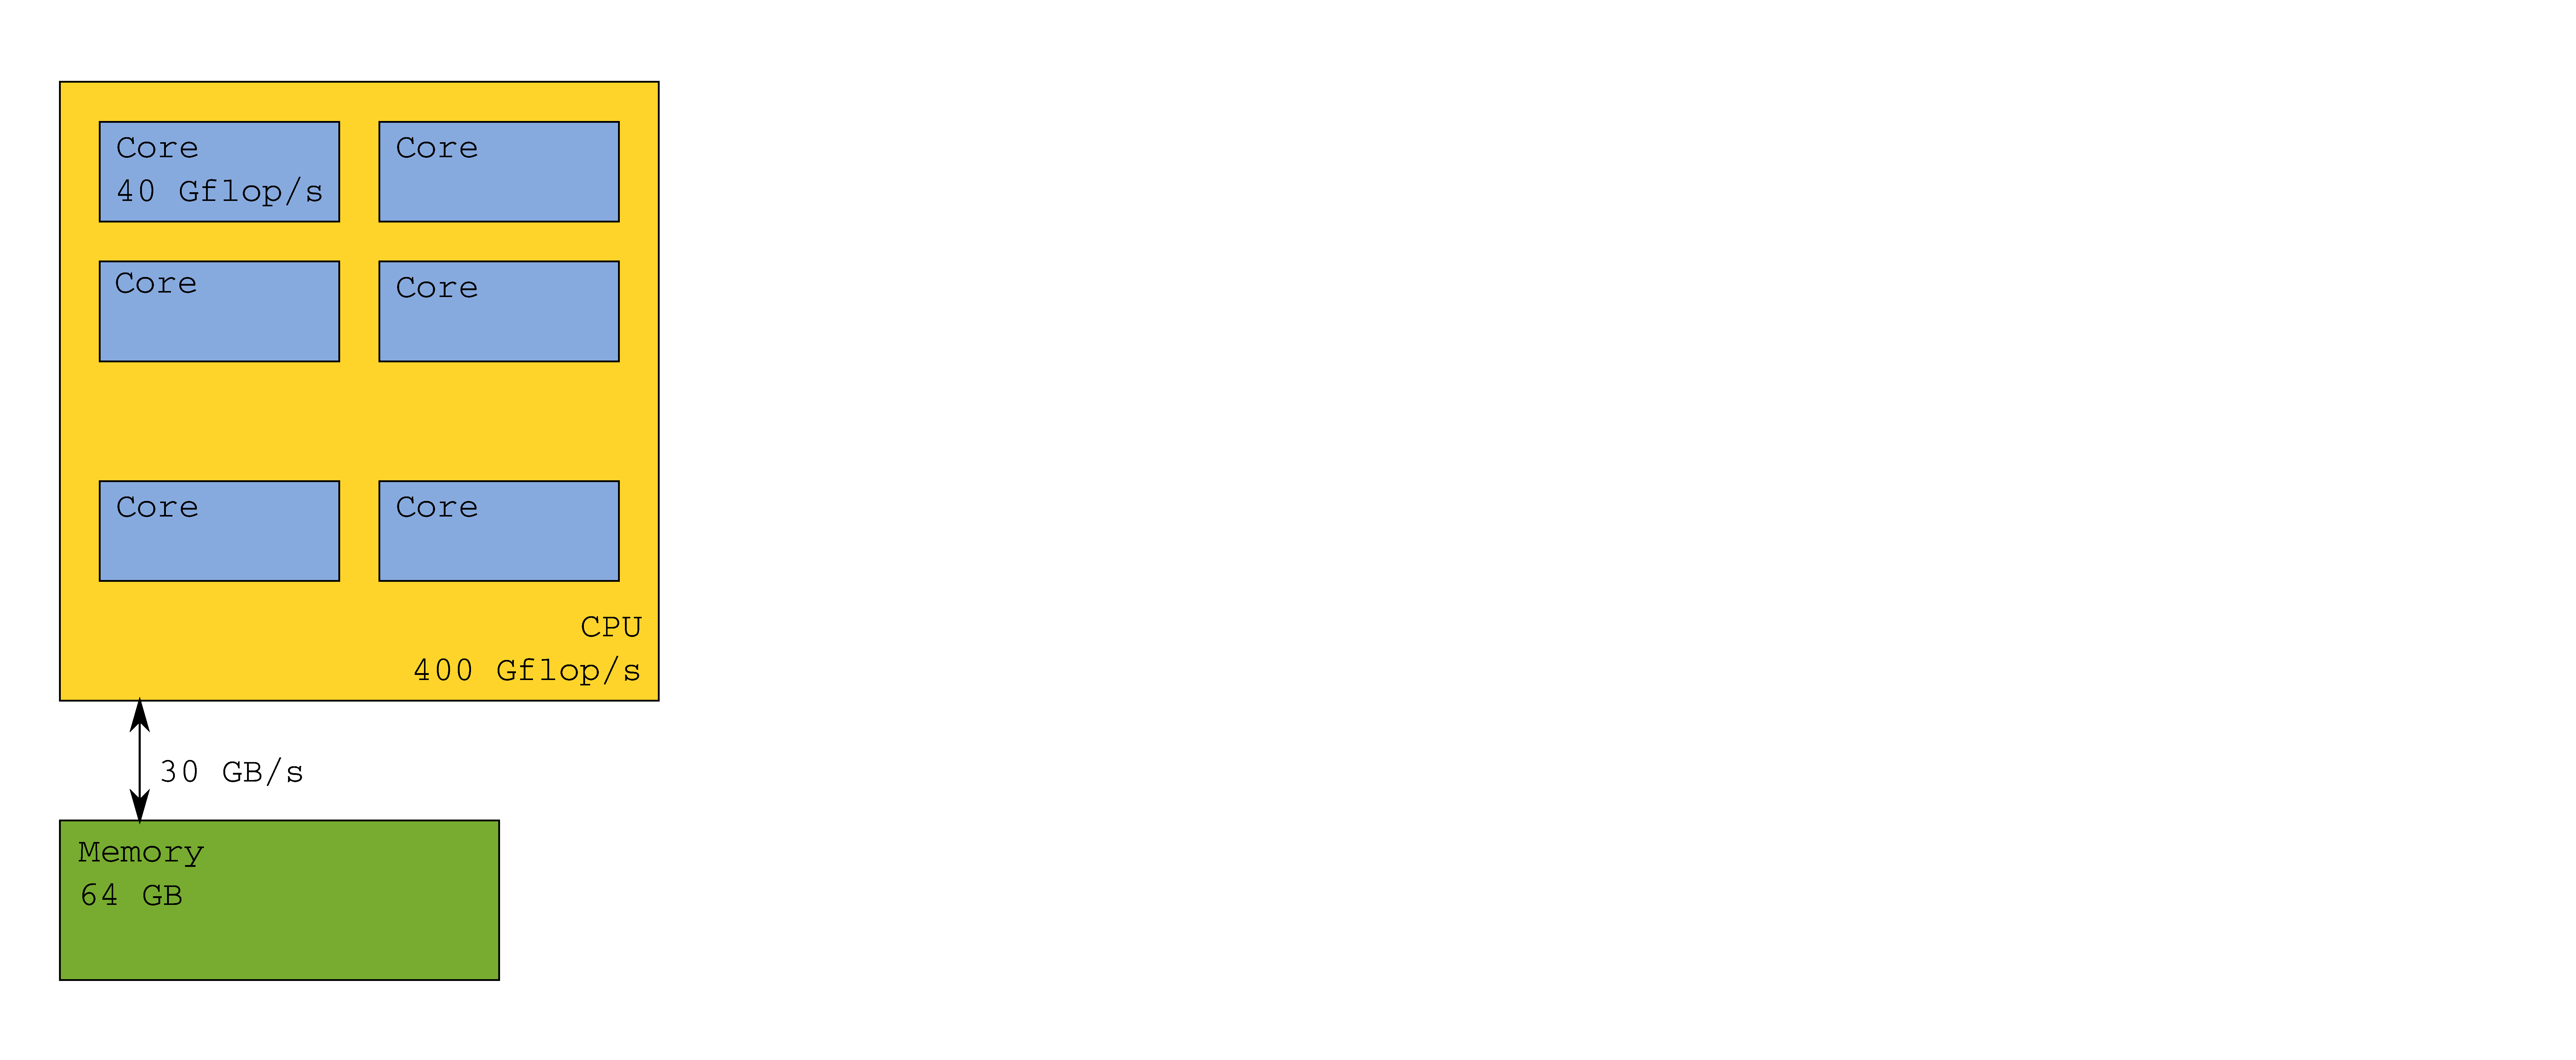
\includegraphics[width=0.9\textwidth]{figures/hpc-arch1}}%
    \only<2>{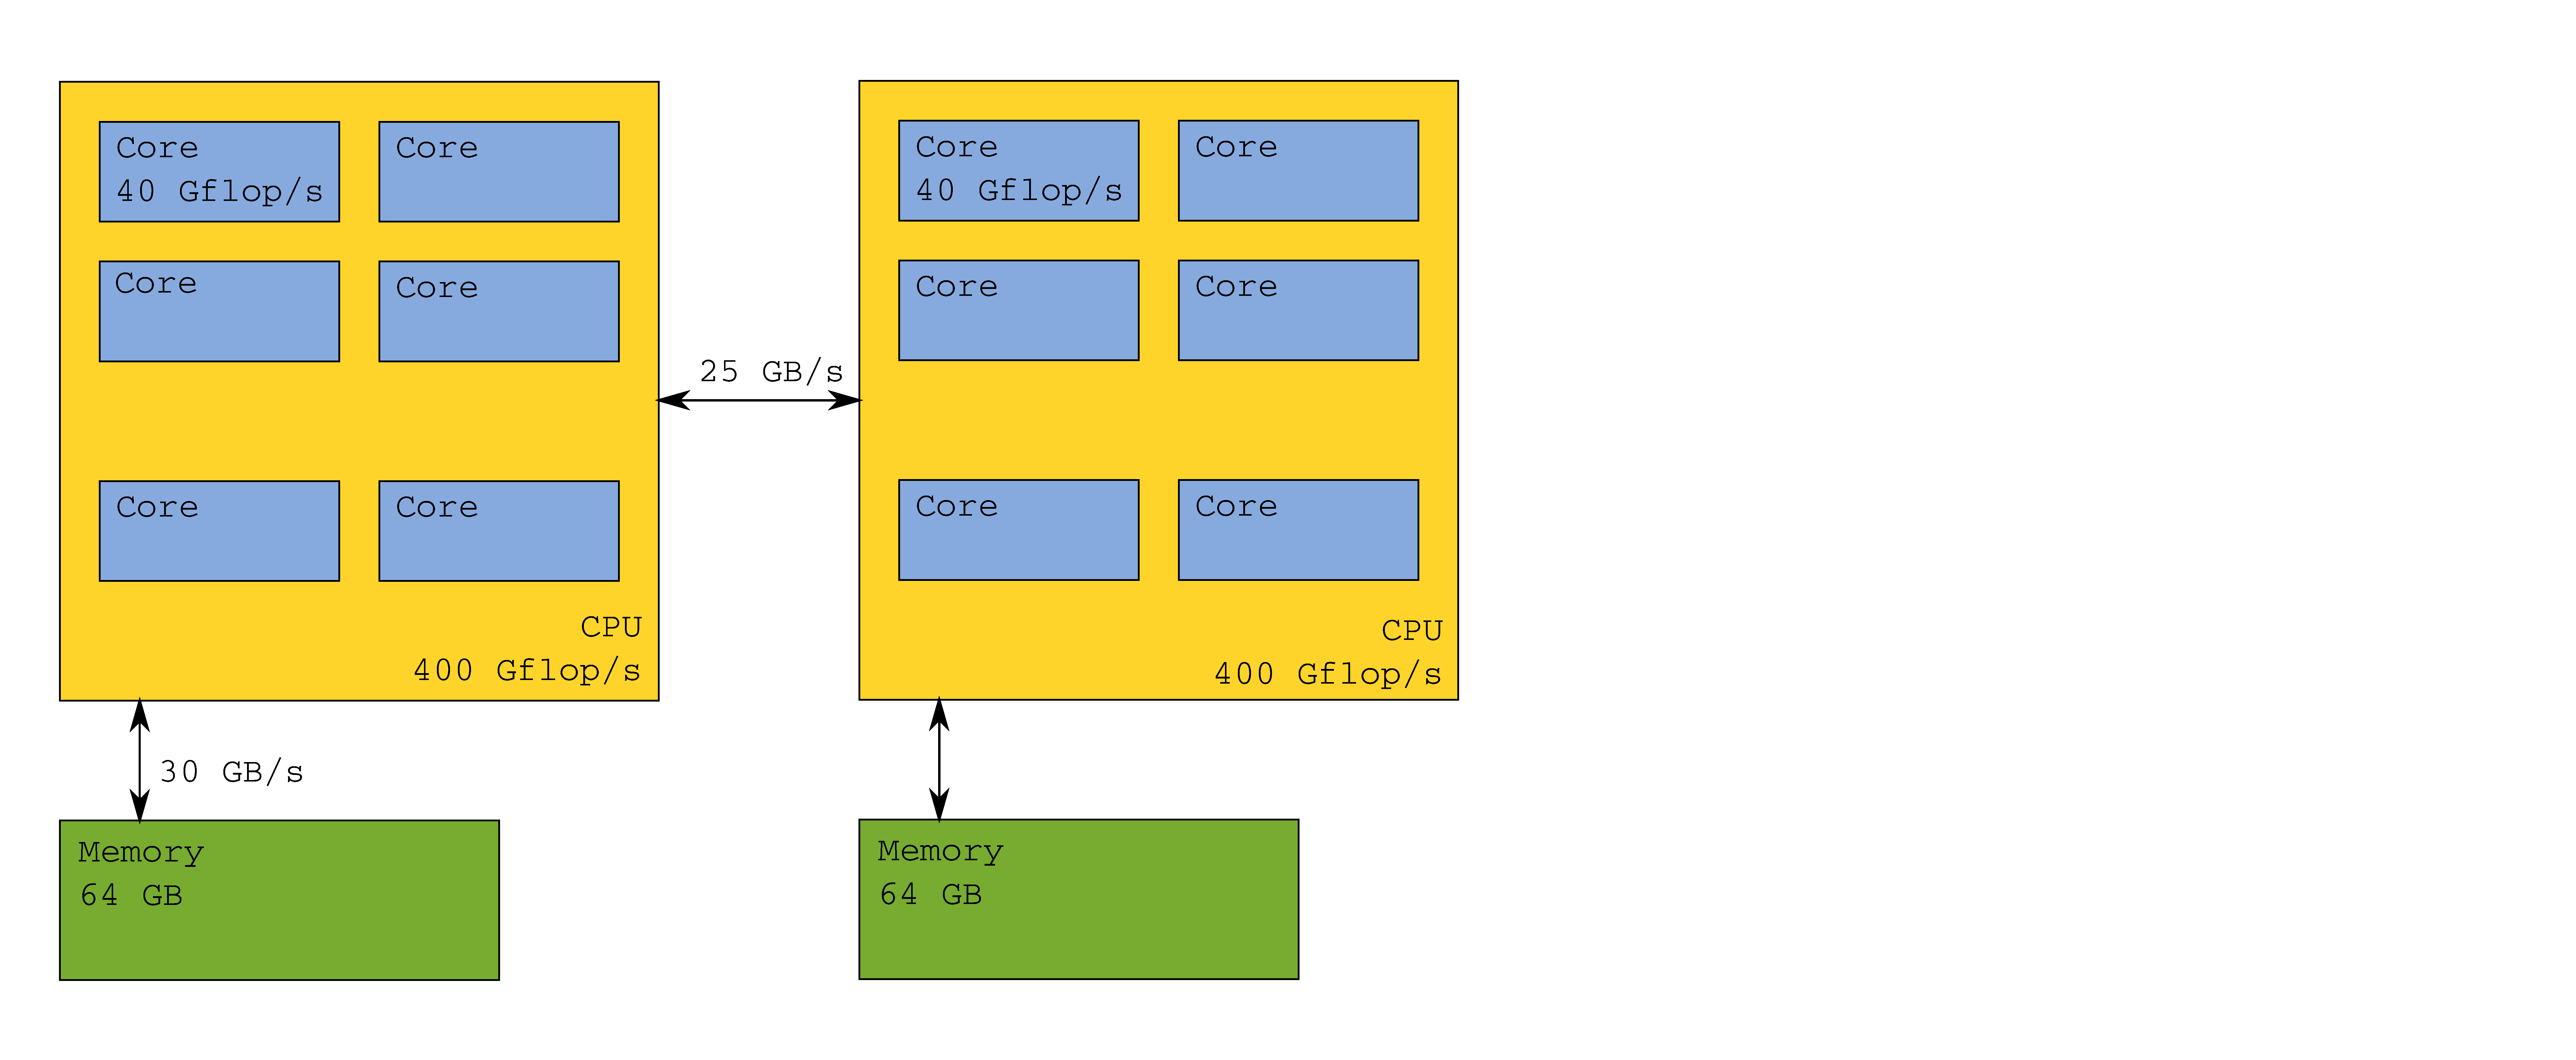
\includegraphics[width=0.9\textwidth]{figures/hpc-arch2}}%
    \only<3>{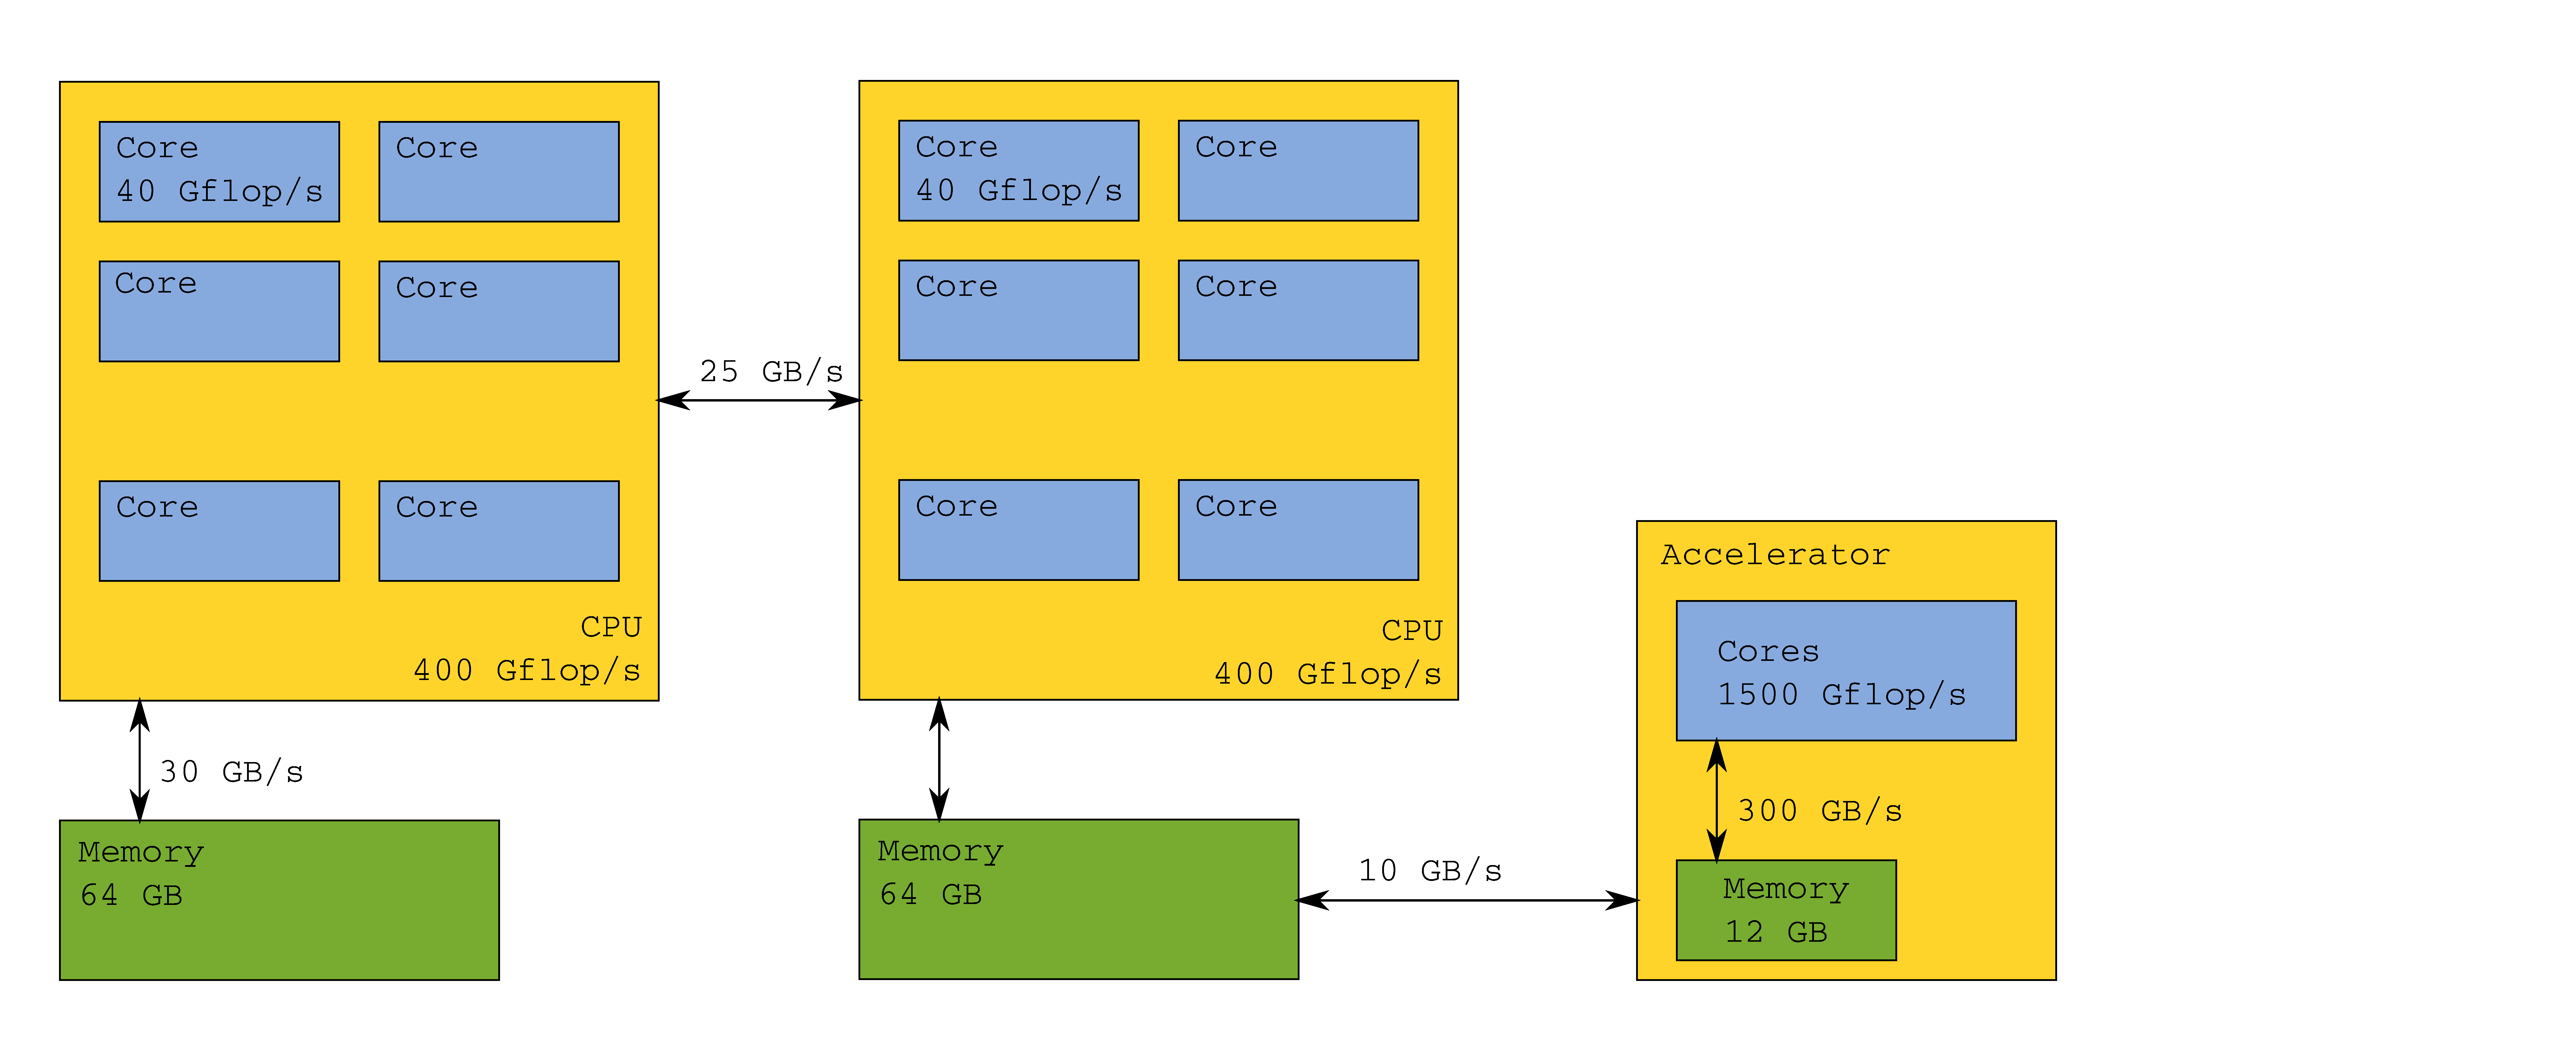
\includegraphics[width=0.9\textwidth]{figures/hpc-arch3}}%
    \only<4->{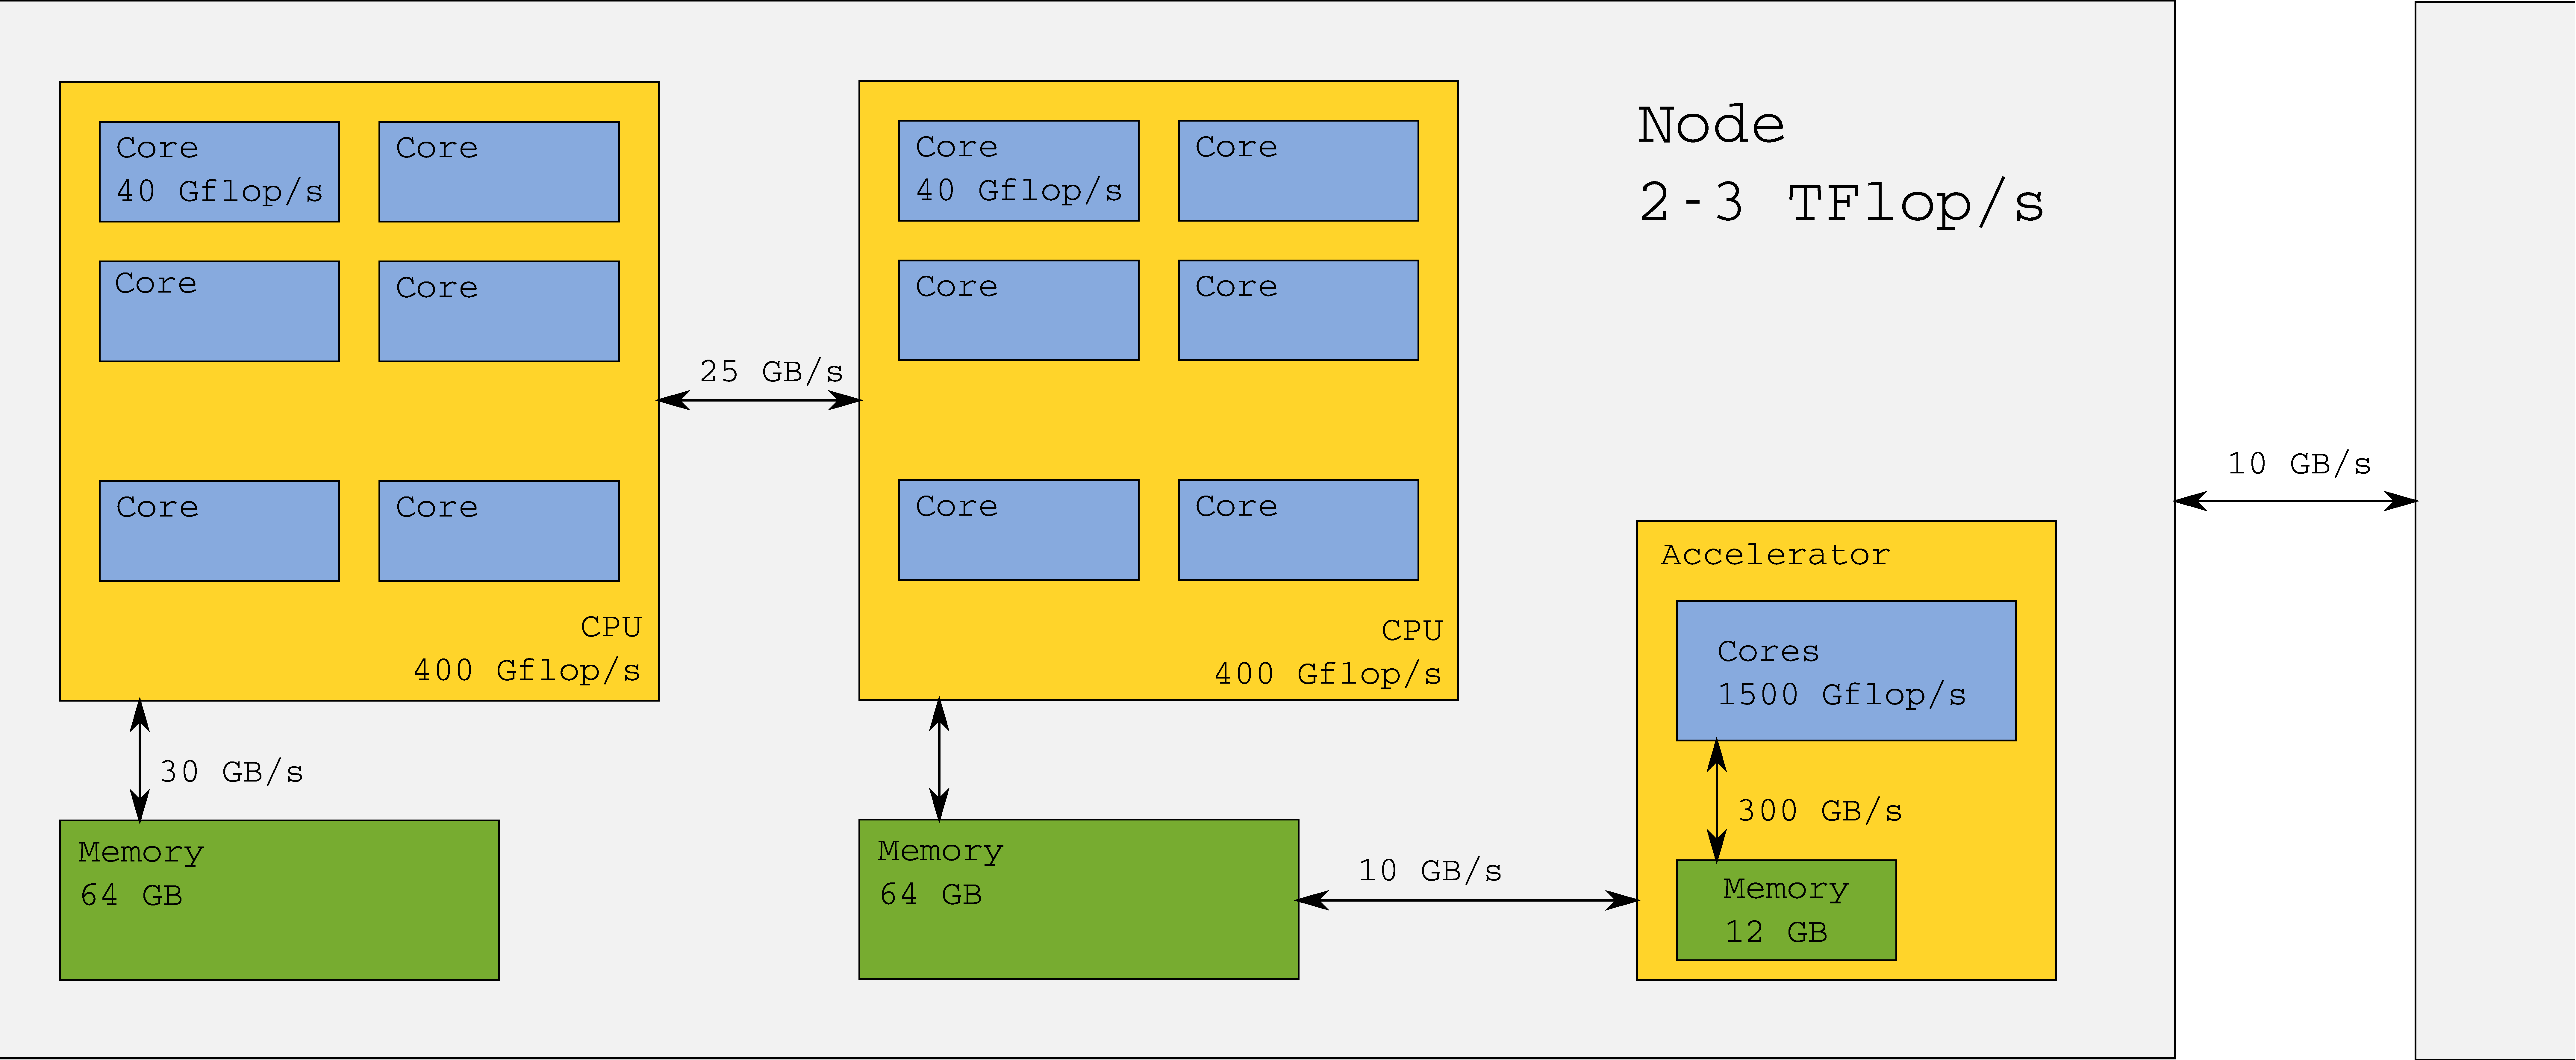
\includegraphics[width=0.9\textwidth]{figures/hpc-arch4}}%
  \end{center}
    
  Typical HPC computing platforms are equipped with
  multiple nodes, connected through a high speed network, with at
  each nodes:
  \begin{itemize}
  \item<1-> \dr{multicore processors} connected to a NUMA memory node.
  \item<3-> one or more \dr{accelerators}.
  \end{itemize}
  \uncover<5>{Current HPC platform are extremely \db{heterogeneous} with
    diverse resource capabilities and memory speeds offered by these
    architectures.}  

\end{frame}

% \begin{frame}{Architectures}

%   \begin{center}
%    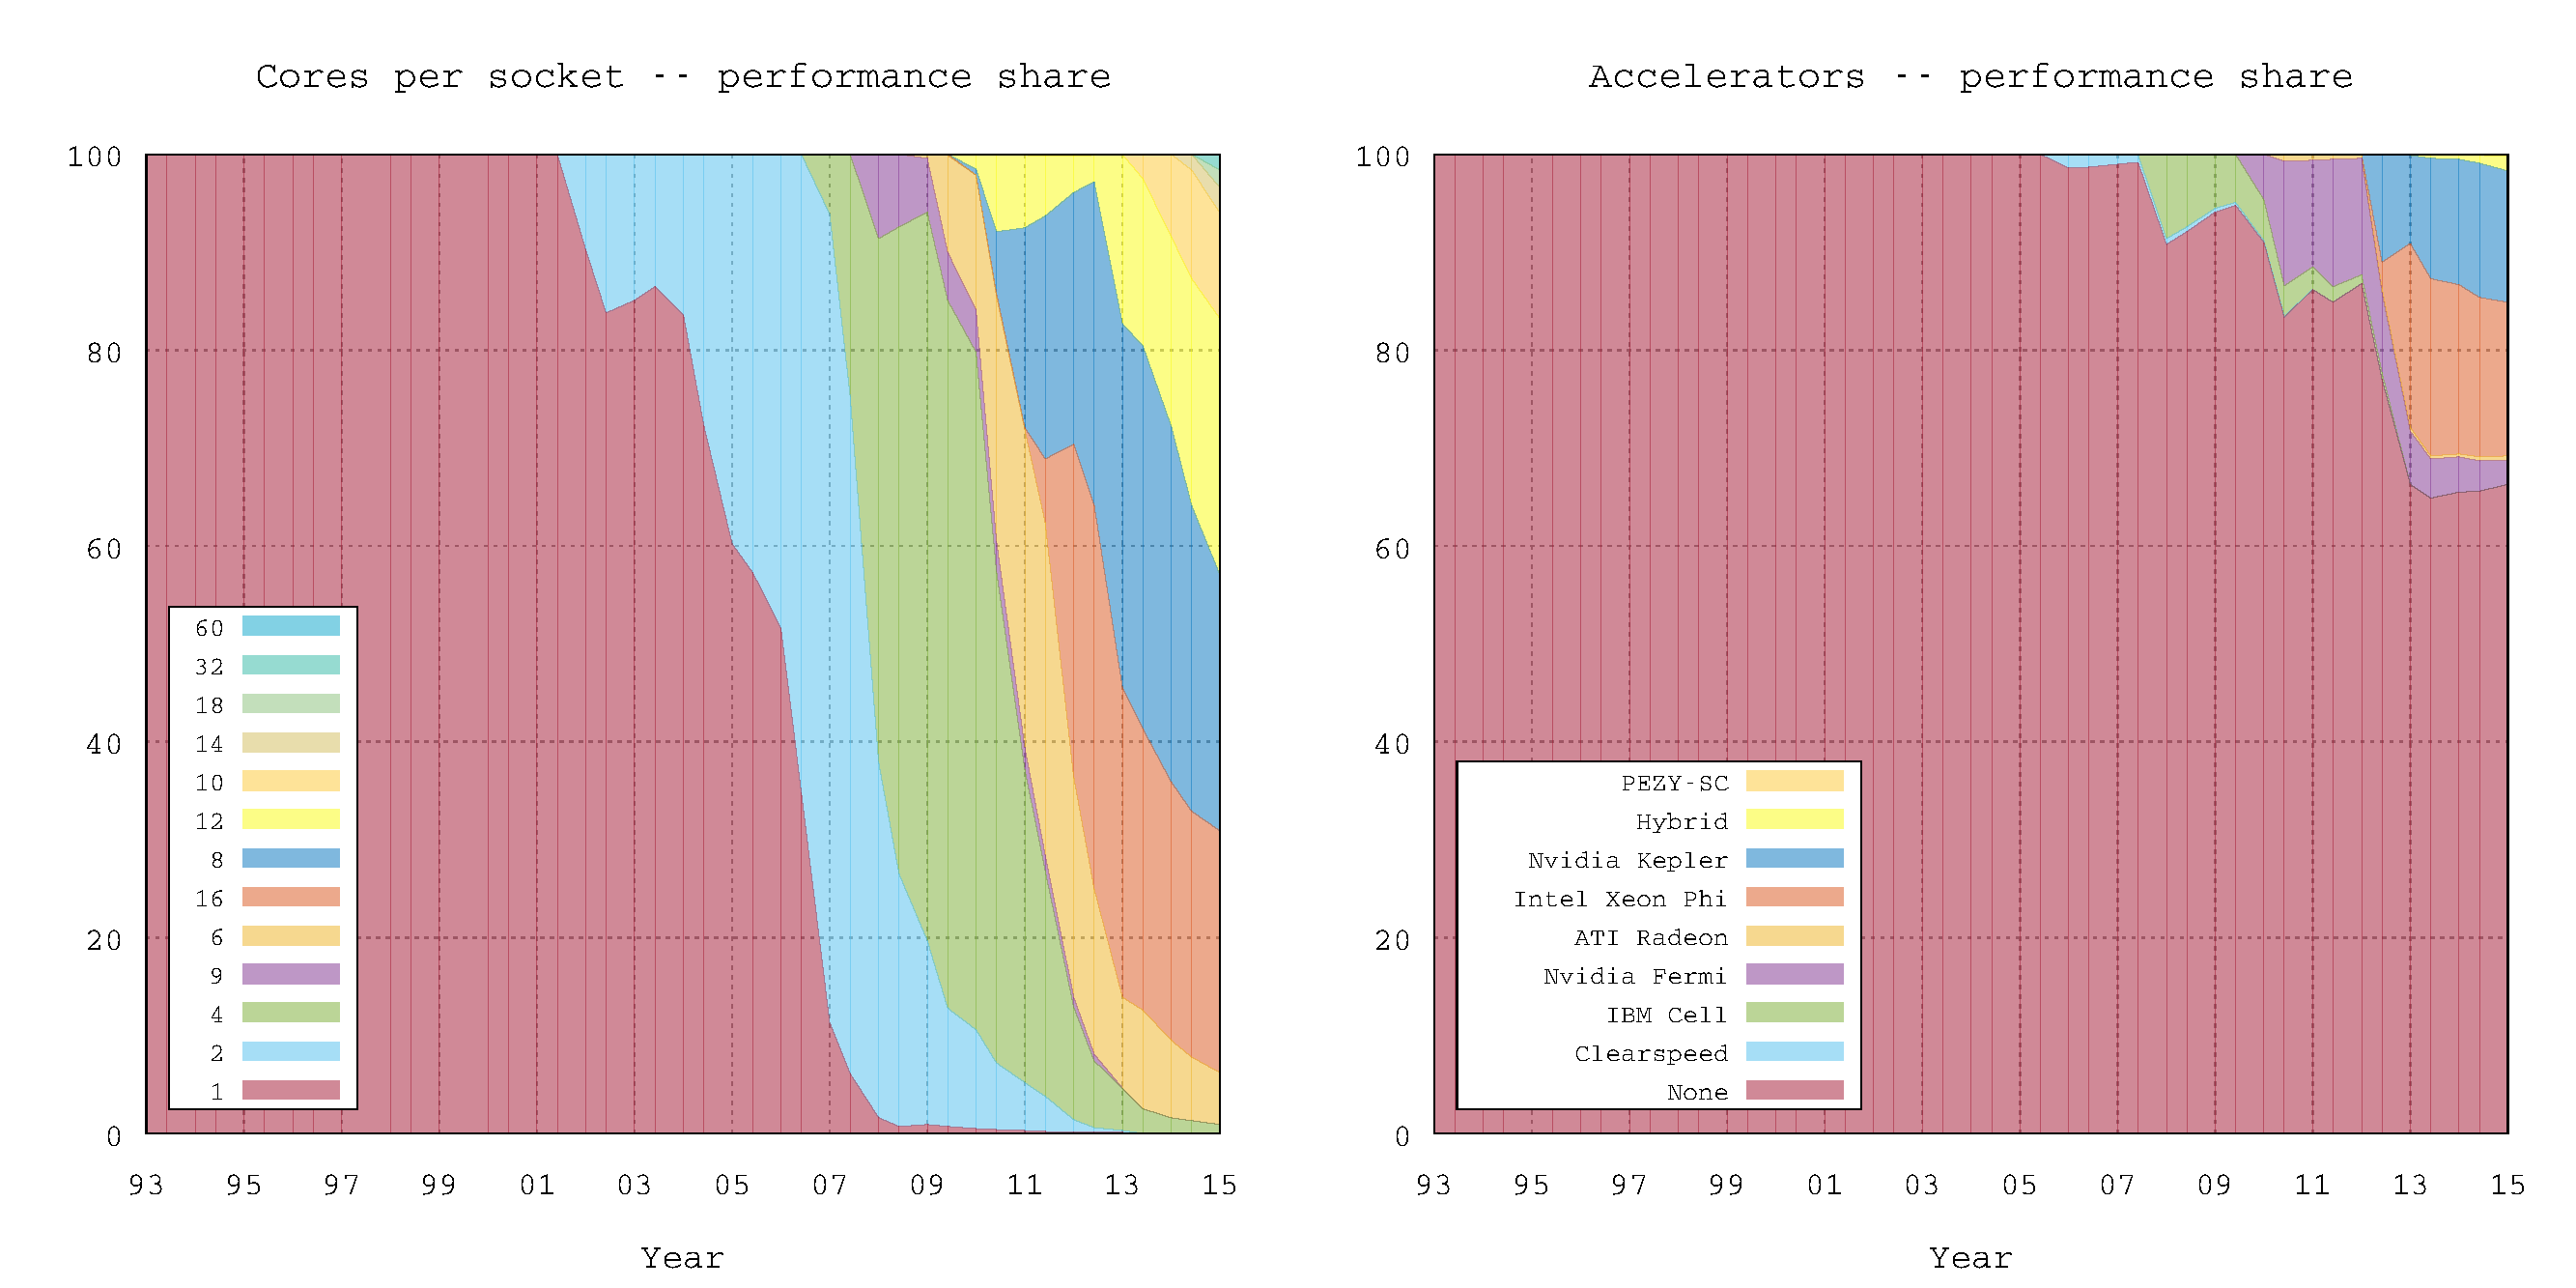
\includegraphics[width=0.9\textwidth]{top500}
%   \end{center}

%   According to the \dr{Top500 lists}, multicore
%   architectures introduced in 2001 nowadays represents 100 \% of
%   the performance share in the list. Accelerator, such as \db{GPU}
%   and \db{Xeon Phi devices}, started gaining interests in the HPC
%   community in 2005 and became very popular ever since.

% \end{frame}

\begin{frame}{Runtime systems}
  \begin{columns}
    \begin{column}{0.45\textwidth}
      \center
      \only<1>{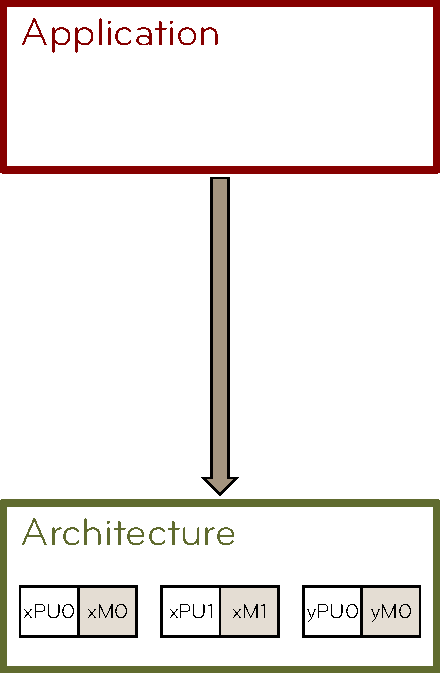
\includegraphics[width=\textwidth]{figures/rt_layers1}}%
      \only<2->{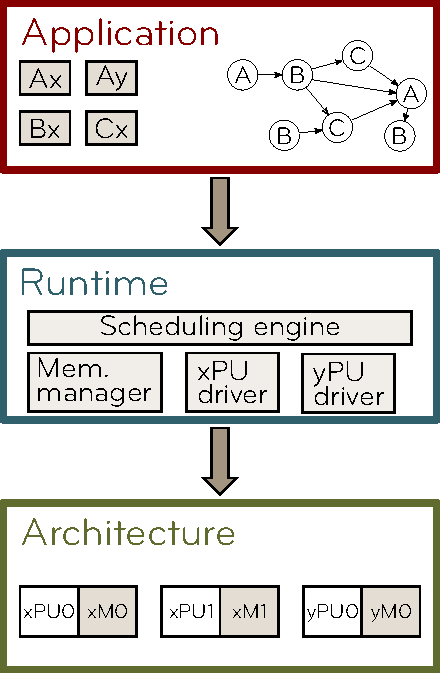
\includegraphics[width=\textwidth]{figures/rt_layers2}}%
    \end{column}
    \begin{column}{0.55\textwidth}
      \begin{itemize}
      \item<1->The classical approach is based on a mixture of
        technologies (e.g., MPI+OpenMP+CUDA) which.
        \begin{itemize}
        \item requires a big programming effort.
        \item is difficult to maintain and update.
        \item is prone to (performance) portability issues.
        \end{itemize}
      \item<2-> \dr{runtimes} provide an abstraction layer that hides
        the architecture details.
      \item<3-> the workload is expressed as a \dr{DAG} (Directed
        Acyclic Graph) of tasks.
        % where the dependencies are
        % \begin{itemize}
        % \item<3-> defined explicitly
        % \item<3-> defined through rules
        % \item<3-> automatically inferred
        % \end{itemize}
      \end{itemize}
    \end{column}
  \end{columns}
\end{frame}

\begin{frame}{Runtime systems and programming models}

  This approach has been assessed in the domain of \dr{dense
  linear algebra} and still represents a challenge for \dr{sparse
  algorithms}.

  \begin{itemize}
  \item \dr{Programming models}: \\ \db{Sequential Task Flow (STF)},
    Parametrized Tasks Graph (PTG) % recurssive, call-back
  \item \dr{Runtime systems}: \\ \db{StarPU}, PaRSEC, QUARK, KAAPI, StarSS,
    SuperGlue
  \item \dr{Research project}: \\ \db{SOLHAR (ANR-MN)}, NLAFET
    (H2020), INTERTWinE (H2020), SparseKafe (NSF)
  \item \dr{Scientific libraries}: \\ \texttt{qr\_mumps}, PasTiX,
    Chameleon, (D)PLASMA
  \end{itemize}

  \vspace{0.3cm}

  \uncover<2>{Recently added features of the OpenMP standard have been inspired by
  these efforts:
  \begin{itemize}
  \item OpenMP 3.0: the \texttt{task} construct
  \item OpenMP 4.0: the \texttt{depend} clause and
    \texttt{target} construct
  \item OpenMP 4.5: the \texttt{priority} clause
  \end{itemize}}

\end{frame}

\begin{frame}{Position of the thesis}

  \vspace{0.3cm}
  
  \begin{block}{Challenges}
    Achieve an efficient and portable implementation of a sparse,
    direct method, improve it by integrating new advanced features and
    achieve the porting on heterogeneous architectures.
  \end{block}

  \vspace{0.3cm}

  % \uncover<2->{Exploiting a pure \dr{STF} model on top of a modern \dr{runtime
    % system}:}
  \uncover<2->{Use a task-based parallel paradigm trough a
    \dr{runtime system}:}

  \vspace{0.1cm}

  \begin{itemize}
  % \item<2-> Improve the scalability of a sparse direct solver by
  %   introducing 2D, Communication Avoiding front factorization
  %   algorithms.
  \item<2-> Improve the scalability of a sparse direct solver by
    introducing 2D, Communication Avoiding algorithms.
  \item<3-> Devise algorithms for efficiently exploit the capabilities
    of \dr{heterogeneous systems}.
  \item<4-> Design and implement a reliable and efficient \alert{memory-aware}
    algorithm for controlling the memory consumption of the solver
    during a parallel execution.
  \item<5-> Develop tools for \alert{analyzing and evaluating} the performance and
    scaling of a parallel application on heterogeneous systems.
  \end{itemize}
  
\end{frame}

%%% Local Variables:
%%% mode: latex
%%% TeX-master: "defense"
%%% TeX-engine: xetex
%%% End:

% \section{Performance analysis approach}
% \input{analysis}
\section{Task-based multifrontal QR method}
\begin{frame}{The Multifrontal QR method}
  \begin{overlayarea}{\textwidth}{1cm}
    \only<1>{The original \dr{multifrontal method} by Duff \&
        Reid '83 can be extended to \dr{QR} factorization of sparse
      matrices.

      This method is guided by a graph called \alert{\it elimination
        tree}:}%
    \only<2-3>{The tree is traversed in \db{topological order} (i.e.,
      bottom-up) and, at each node, two operations are performed:}%
    \only<4->{Typically \dr{two sources of parallelism} are exploited
      in the multifrontal method}
  \end{overlayarea}

  \vspace{0.2cm}

  \begin{columns}
    \begin{column}{0.6\textwidth}
      \begin{overlayarea}{\textwidth}{6cm}
        \only<1>{\begin{itemize}
          \item each node is associated with a relatively small
            \alert{dense} matrix called \db{frontal matrix} (or
            \db{front}) containing k pivots to be eliminated along
            with all the other coefficients concerned by their
            elimination.
          \end{itemize}}\only<2-3>{
          \begin{itemize}
          \item<2-3> \alert{assembly}: coefficients from the original
            matrix associated with the pivots and  \alert{\it
              contribution blocks} produced by the treatment of the child
            nodes are \alert{stacked}  to form the frontal matrix.
          \item<3-> \alert{factorization}: the $k$ pivots are eliminated
            through a complete dense QR factorization of the frontal matrix. As a
            result we get:
            \begin{itemize}
            \item part of the global $R$ and $Q$ factors.
            \item a triangular \db{\it contribution block} that will be
              assembled into the father's front.
            \end{itemize}
            
          \end{itemize}}\only<4->{\begin{itemize}
          \item<5-> \dr{tree-level} parallelism: frontal matrices located in
            independent branches in the tree can be processed in
            parallel.
          \item<6-> \dr{node-level} parallelism: large frontal matrices
            factorization may be performed in parallel by multiple
            threads.
          \end{itemize}}
      \end{overlayarea}
    \end{column}
    \begin{column}{0.4\textwidth}
      \begin{center}
        \only<1>{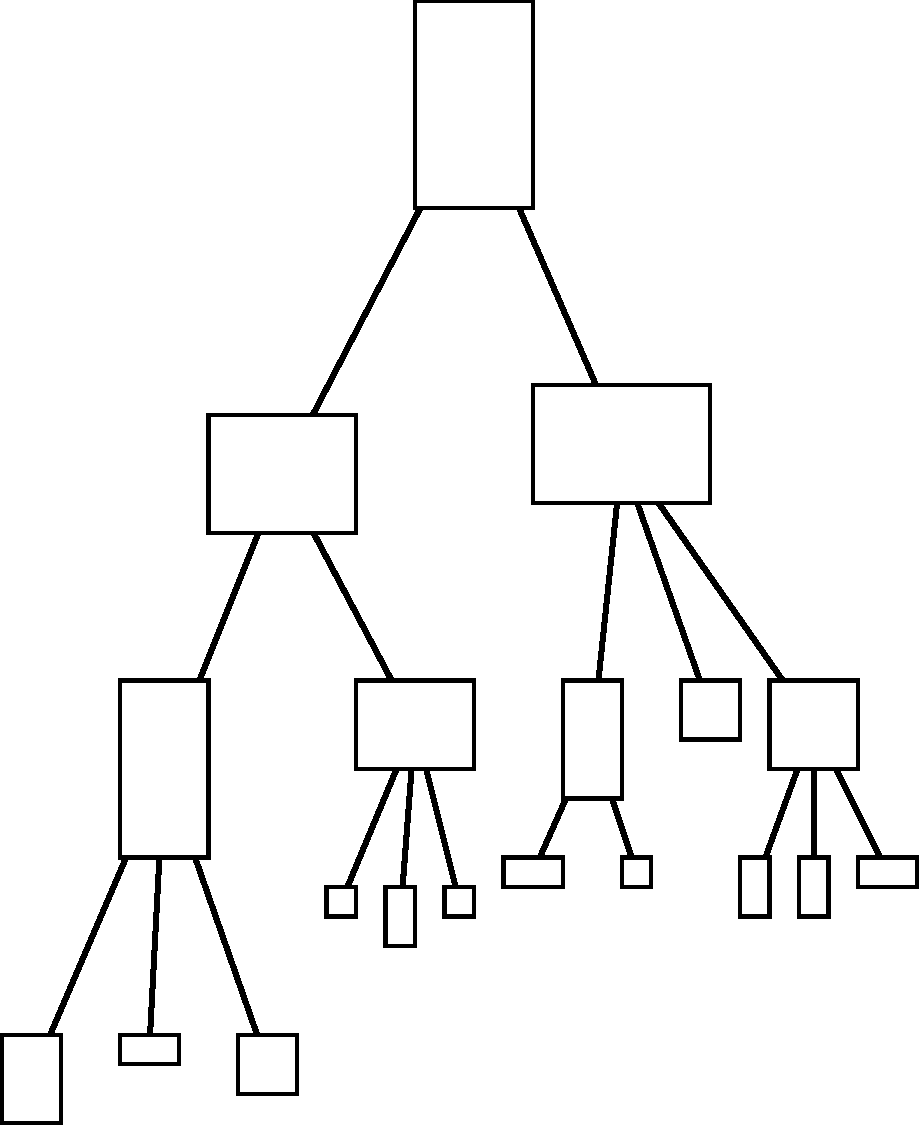
\includegraphics[width=\textwidth]{figures/etree}}%
        \only<2>{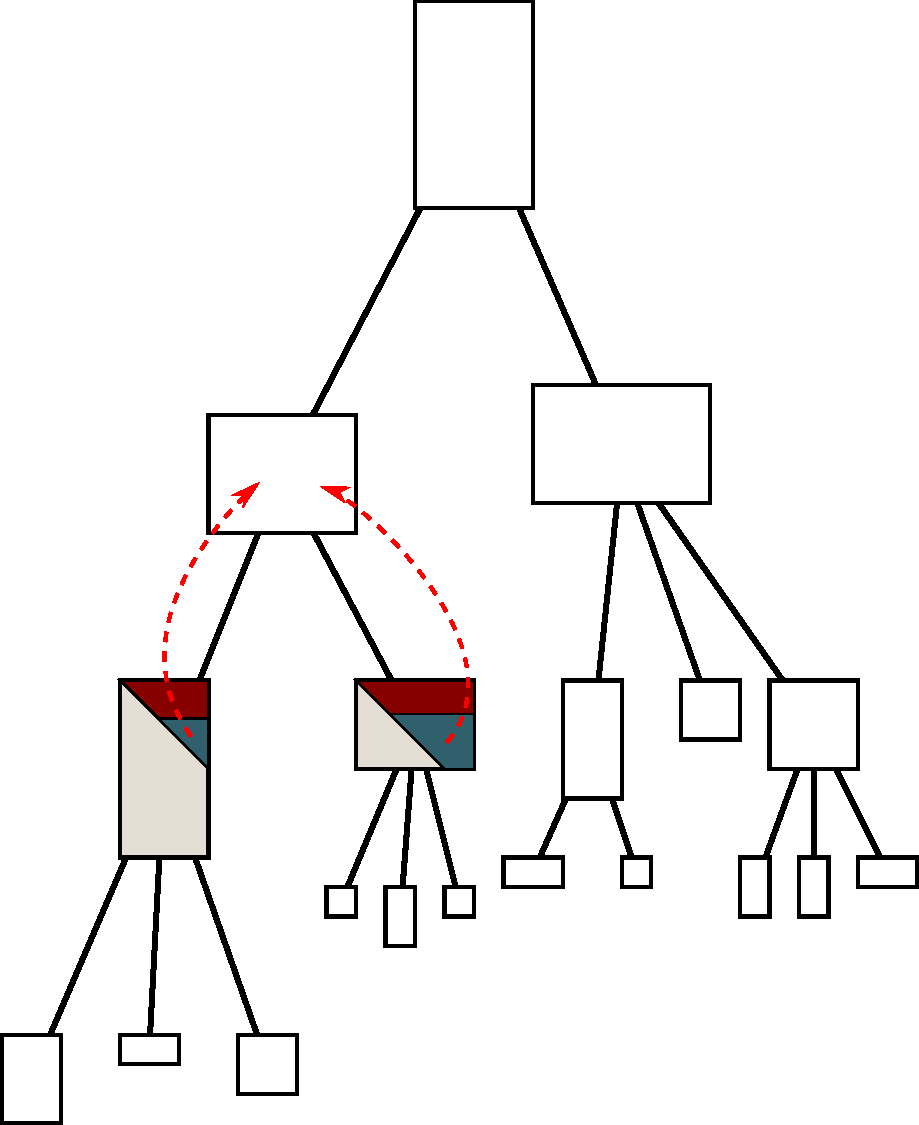
\includegraphics[width=\textwidth]{figures/etree2}}%
        \only<3->{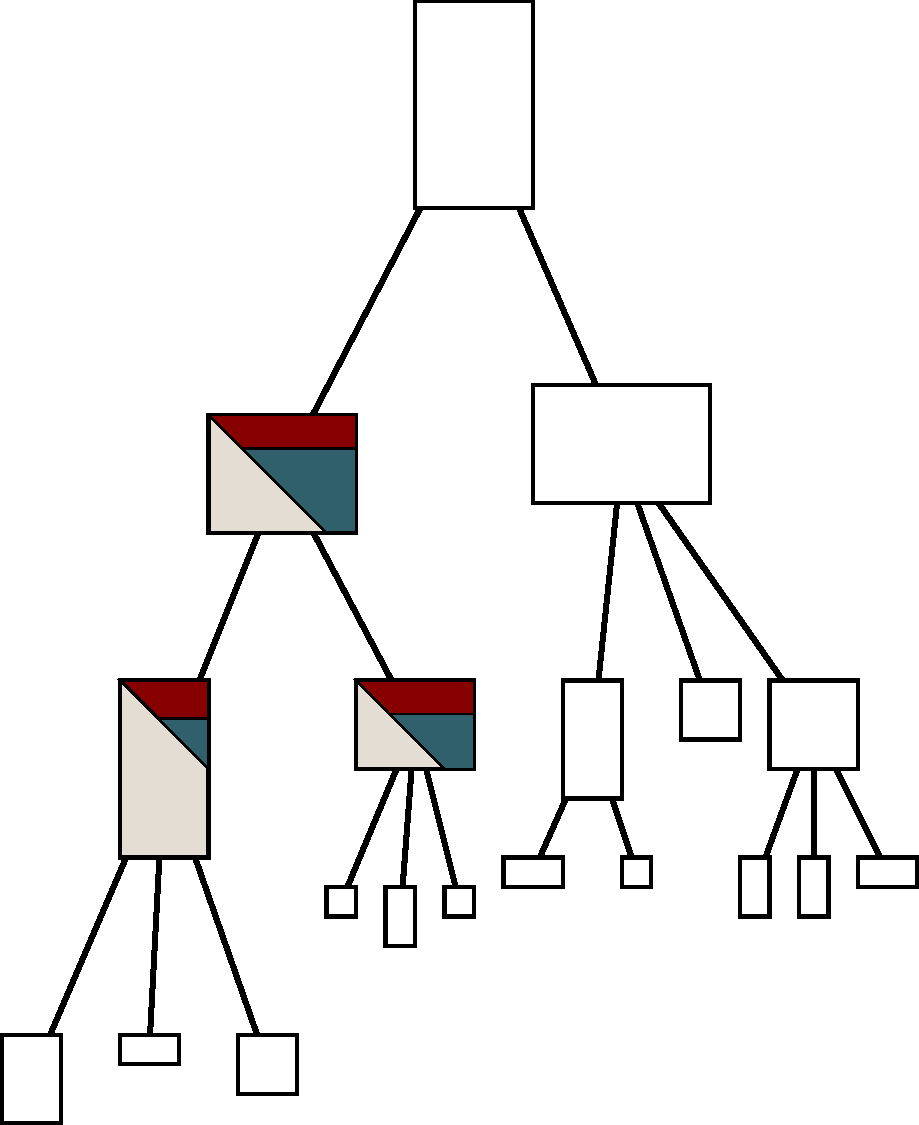
\includegraphics[width=\textwidth]{figures/etree3}}%
      \end{center}
    \end{column}
  \end{columns}
\end{frame}

\begin{frame}[fragile,t]{The task-based multifrontal QR factorization}
  \dr{Sequential} multifrontal $QR$ code

  \begin{columns}[t]
    \begin{column}{0.45\textwidth}
      \begin{center}
        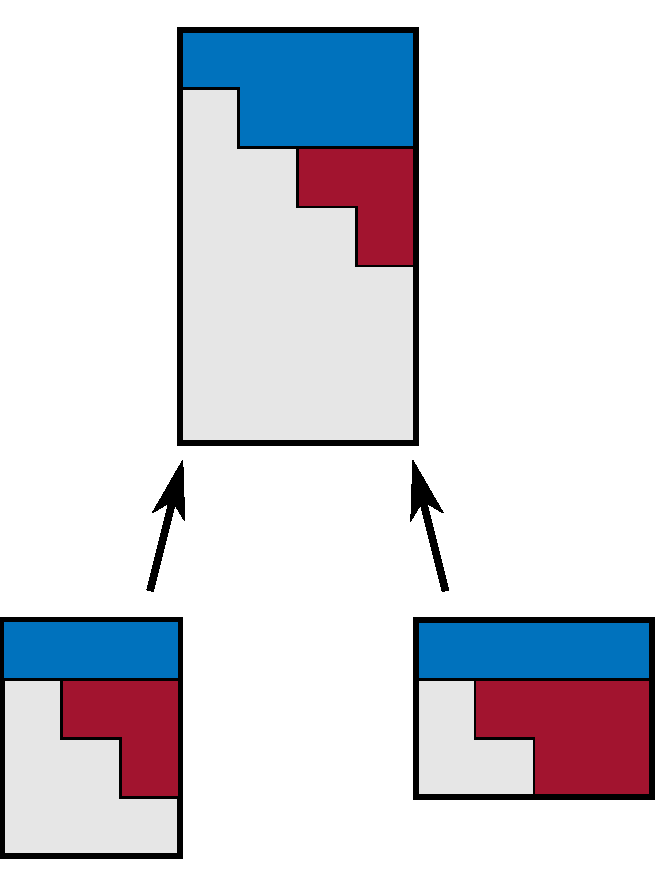
\includegraphics[width=0.6\textwidth]{figures/tree}
      \end{center}
    \end{column}
    \begin{column}{0.55\textwidth}
      \lstinputlisting{listings/mf-seq.f90}
    \end{column}
  \end{columns}
\end{frame}

\begin{frame}[fragile,t]{The task-based multifrontal QR factorization}
  \dr{Sequential} multifrontal $QR$ code with 1D block partitioning

  \begin{columns}[t]
    \begin{column}{0.45\textwidth}
      \begin{center}
        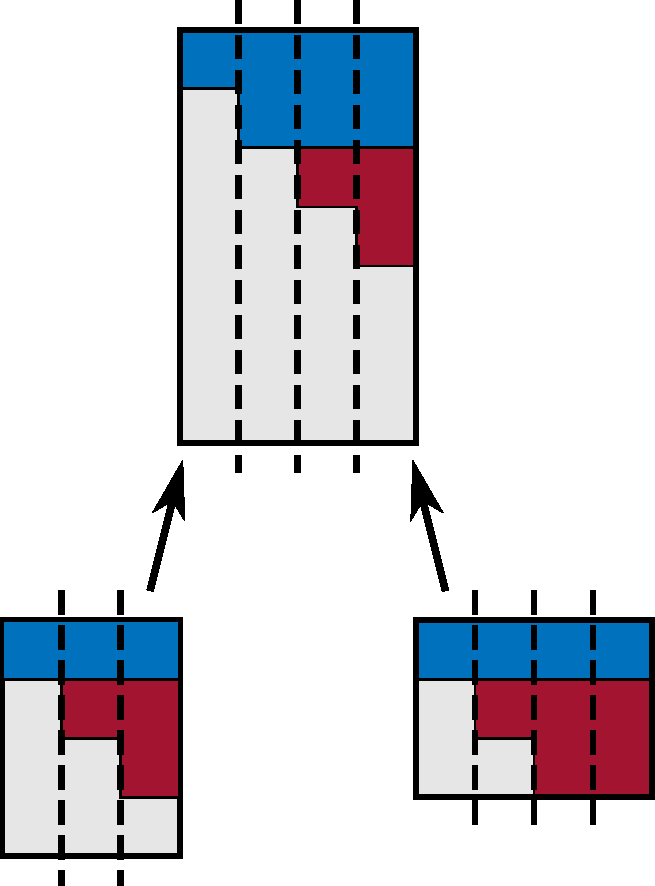
\includegraphics[width=0.6\textwidth]{figures/tree_part}
      \end{center}
    \end{column}
    \begin{column}{0.55\textwidth}
      \lstinputlisting{listings/mf-seq-multicore.f90}
    \end{column}
  \end{columns}
\end{frame}

\begin{frame}[fragile,t]{The task-based multifrontal QR factorization}
The tree is transformed into a DAG

\begin{columns}[t]
  \begin{column}{0.45\textwidth}
    \begin{center}
      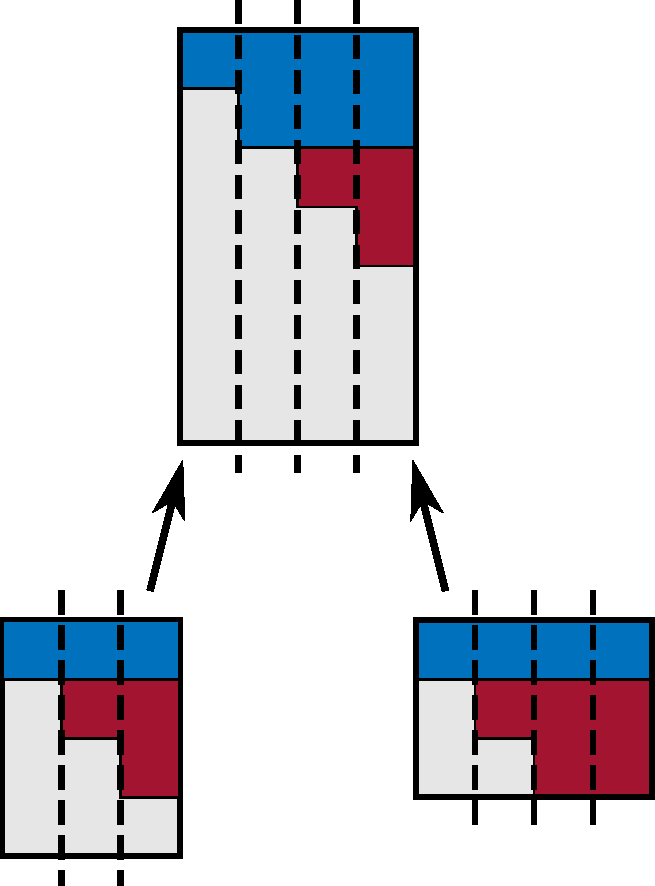
\includegraphics[width=0.6\textwidth]{figures/tree_part}
    \end{center}
  \end{column}
  \begin{column}{0.55\textwidth}
    \begin{center}
      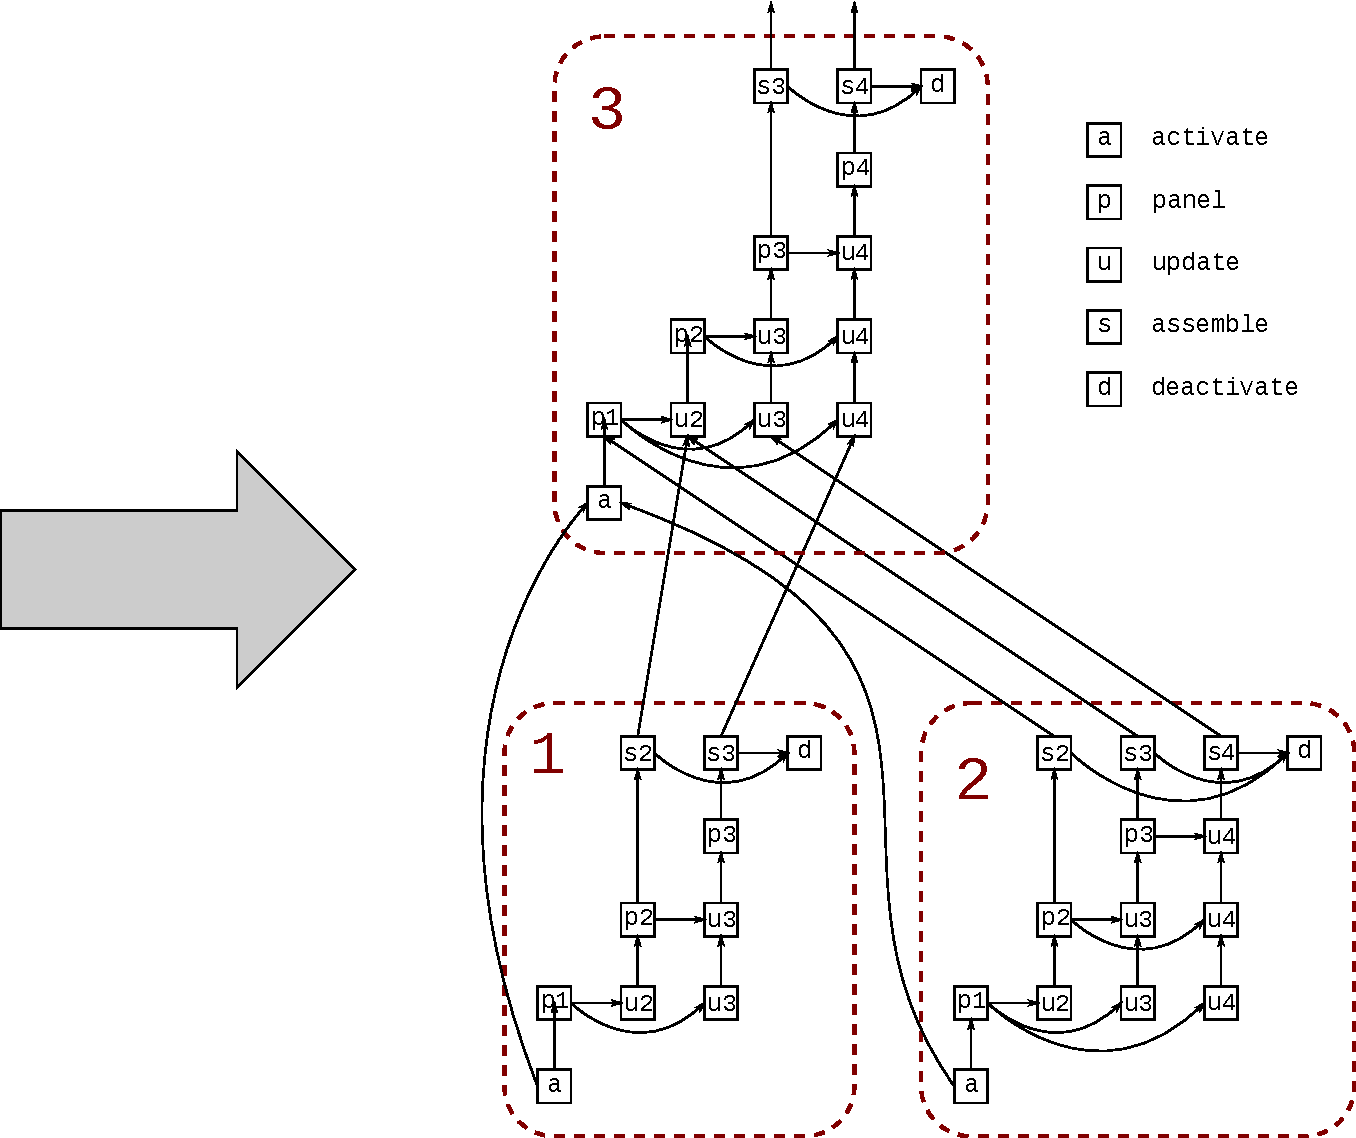
\includegraphics[width=0.8\textwidth]{figures/tree_dag}
    \end{center}
  \end{column}
\end{columns}

\vspace{0.5cm}

\begin{itemize}
\item Seamless exploitation of tree and node parallelism.
\item \alert{Inter-level concurrency} (father-child pipelining).
\end{itemize}

\vspace{0.2cm}

\uncover<2>{This method is implemented in the \texttt{qr\_mumps 1.0} package and
parallelized with OpenMP (2.0).}

\end{frame}

%%% Local Variables:
%%% mode: latex
%%% TeX-master: "defense"
%%% TeX-engine: xetex
%%% End:


\section{STF-based parallel multifrontal QR method for multicore architectures}
\begin{frame}{The Sequential Task Flow model}

  \begin{block}{In the Sequential Task Flow (STF) model:}

    \begin{itemize}
    \item The parallel code looks exactly the same as the sequential one
      except that operations are not executed but
      \alert{submitted} to the system in the form of \alert{tasks}
    \item Depending on how tasks access data and on the (sequential) order of submission,
      the runtime infers dependencies among them and builds a DAG
    \item The runtime scheduler deploys the DAG on the
      underlying architecture
    \item The runtime memory manager moves data from one memory to
      another and maintains the global memory coherency
    \item Equivalent to \alert{Superscalar} techniques in microprocessors
    \end{itemize}

  \end{block}

  \vspace{0.2cm}

  Runtimes relying on STF: \alert{StarPU}, QUARK, SMPss, OpenMP 4.0

\end{frame}


\begin{frame}{The STF model: a simple example}

  \begin{columns}
    \begin{column}{0.6\textwidth}
      \begin{block}{Sequential code}
        \texttt{sub\_a(x,y); \gn{// R and W x and y}}\\
        \texttt{sub\_b(x); ~~\gn{// R x} }\\
        \texttt{sub\_c(y); ~~\gn{// R y} }\\
        \texttt{sub\_d(x,y); \gn{// R and W x and y}}\\
      \end{block}

      \vspace{0.5cm}

      \begin{exampleblock}{Equivalent STF code}
        \uncover<2->{\texttt{\alert{submit}(sub\_a,x:\alert{RW},y:\alert{RW});}}

        \uncover<3->{\texttt{\alert{submit}(sub\_b,x:\alert{R});              }}

        \uncover<4->{\texttt{\alert{submit}(sub\_c,y:\alert{R});              }}

        \uncover<5->{\texttt{\alert{submit}(sub\_d,x:\alert{RW},y:\alert{RW});}}

        \uncover<6->{\texttt{\alert{wait\_tasks\_completion}( );}}
      \end{exampleblock}
    \end{column}
    \begin{column}{0.4\textwidth}
      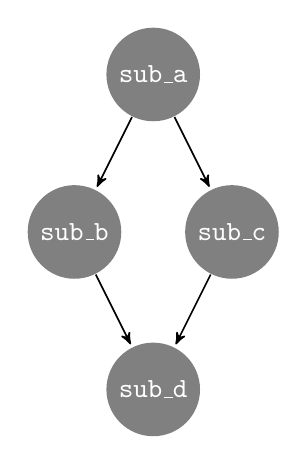
\begin{tikzpicture}[->,>=stealth',shorten >=1pt,auto,node distance=2.8cm,
        semithick]
        \tikzstyle{every state}=[fill=gray,draw=none,text=white]

        \uncover<2->{\node[state]     (A) at (2,5)  {\texttt{sub\_a}};}
        \uncover<3->{\node[state]     (B) at (1,3)  {\texttt{sub\_b}};}
        \uncover<4->{\node[state]     (C) at (3,3)  {\texttt{sub\_c}};}
        \uncover<5->{\node[state]     (D) at (2,1)  {\texttt{sub\_d}};}

        \uncover<3->{\path (A) edge  (B); }
        \uncover<4->{\path (A) edge  (C); }
        \uncover<5->{\path (B) edge  (D); }
        \uncover<5->{\path (C) edge  (D); }
      \end{tikzpicture}
    \end{column}
  \end{columns}

  \vspace{0.5cm}

  \uncover<6->{\texttt{sub\_b} and \texttt{sub\_c} can be executed in \alert{parallel}.}
  \uncover<7->{If \texttt{sub\_a} is executed on CPU and
    \texttt{sub\_b} on GPU, \texttt{x}  will be automatically transferred.}
\end{frame}

\begin{frame}[fragile,t]{The STF parallel multifrontal QR factorization}
  \dr{Sequential} multifrontal $QR$ code with 1D block partitioning

  \begin{columns}[t]
    \begin{column}{0.45\textwidth}
      % \begin{center}
        % 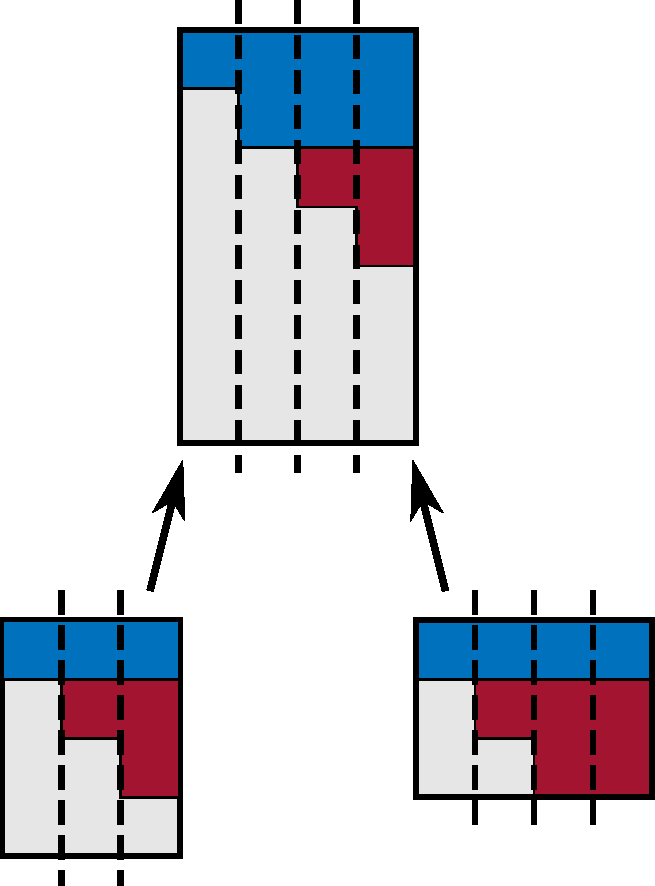
\includegraphics[width=0.6\textwidth]{figures/tree_part}
      % \end{center}
      % \begin{itemize}
      % \item Declare data by registering handles;
      % \item Replace function call with tasks submission;
      % \item Activate operations still performed sequentially;
      % \item Barrier to wait for tasks completion.
      % \end{itemize}
    \end{column}
    \begin{column}{0.55\textwidth}
      \lstinputlisting{listings/mf-seq-multicore.f90}
    \end{column}
  \end{columns}
\end{frame}

\begin{frame}[fragile,t]{The STF parallel multifrontal QR factorization}
  \dr{STF parallel} multifrontal $QR$ code with 1D block partitioning

  \begin{columns}[t]
    \begin{column}{0.45\textwidth}
      % \begin{center}
        % 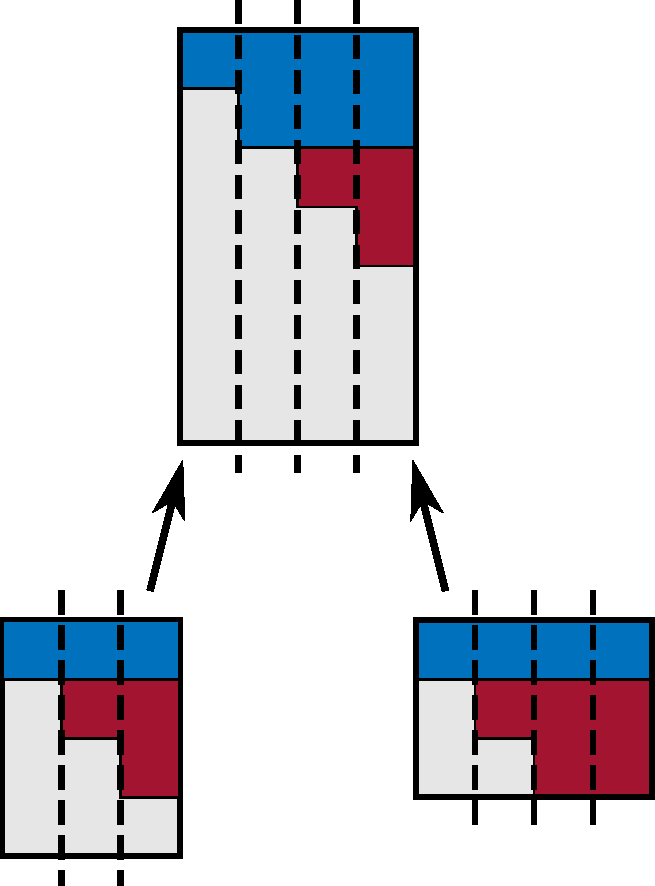
\includegraphics[width=0.6\textwidth]{figures/tree_part}
      % \end{center}
      \begin{itemize}
      \item Declare data by registering handles;
      \item Replace function call with tasks submission;
      \item Activate operations still performed sequentially;
      \item Barrier to wait for tasks completion.
      \end{itemize}
      % \begin{center}
        % 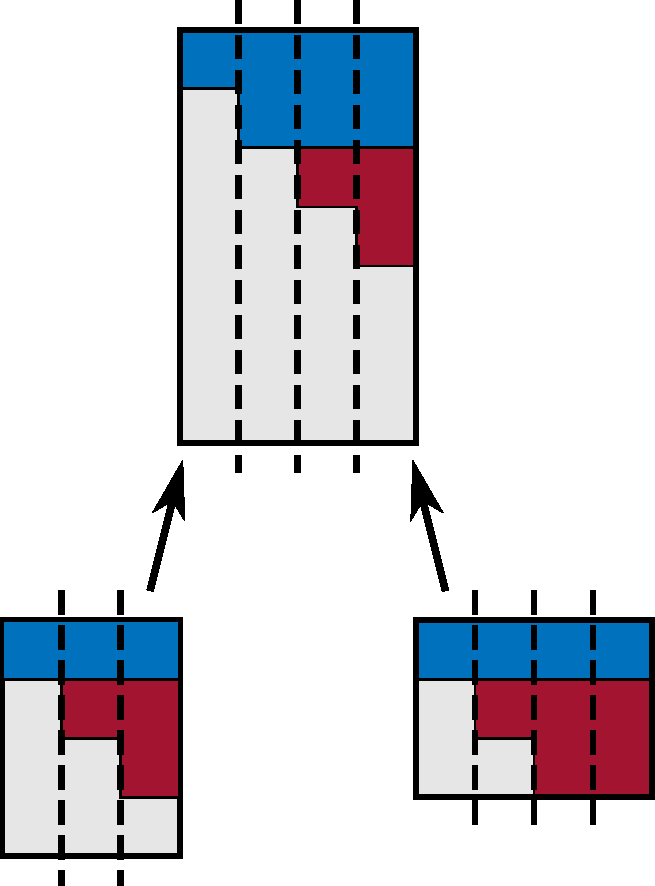
\includegraphics[width=0.6\textwidth]{figures/tree_part}
      % \end{center}
    \end{column}
    \begin{column}{0.55\textwidth}
      \lstinputlisting{listings/mf-stf-multicore.f90}
    \end{column}
  \end{columns}
\end{frame}


\begin{frame}{Experimental results}

  Matrices from the UF SParse Matrix Collection:

  \vspace{0.3cm}

  \begin{center}
    \texttt{\small
      \begin{tabular}{rlrl}
        \hline
        \# & Matrix       & Mflops    & Ordering \\
        \hline
        12 & hirlam       & 1384160   & SCOTCH   \\
        13 & flower\_8\_4 & 2851508   & SCOTCH   \\
        14 & Rucci1       & 5671282   & SCOTCH   \\
        15 & ch8-8-b3     & 10709211  & SCOTCH   \\
        16 & GL7d24       & 16467844  & SCOTCH   \\
        17 & neos2        & 20170318  & SCOTCH   \\
        18 & spal\_004    & 30335566  & SCOTCH   \\
        19 & n4c6-b6      & 62245957  & SCOTCH   \\
        20 & sls          & 65607341  & SCOTCH   \\
        21 & TF18         & 194472820 & SCOTCH   \\
        22 & lp\_nug30    & 221644546 & SCOTCH   \\
        23 & mk13-b5      & 259751609 & SCOTCH   \\
        \hline
      \end{tabular}}
  \end{center}
\end{frame}

\begin{frame}{Experimental results}
  System \db{Ada} (IDRIS supercomputing center):
  \begin{columns}
    \begin{column}{0.5\textwidth}
      % \texttt{\tiny
      %   \begin{tabular}{rlrl}
      %     \hline
      %     \# & Matrix       & Mflops    & Ordering \\
      %     \hline
      %     12 & hirlam       & 1384160   & SCOTCH   \\
      %     13 & flower\_8\_4 & 2851508   & SCOTCH   \\
      %     14 & Rucci1       & 5671282   & SCOTCH   \\
      %     15 & ch8-8-b3     & 10709211  & SCOTCH   \\
      %     16 & GL7d24       & 16467844  & SCOTCH   \\
      %     17 & neos2        & 20170318  & SCOTCH   \\
      %     18 & spal\_004    & 30335566  & SCOTCH   \\
      %     19 & n4c6-b6      & 62245957  & SCOTCH   \\
      %     20 & sls          & 65607341  & SCOTCH   \\
      %     21 & TF18         & 194472820 & SCOTCH   \\
      %     22 & lp\_nug30    & 221644546 & SCOTCH   \\
      %     23 & mk13-b5      & 259751609 & SCOTCH   \\
      %     \hline
      %   \end{tabular}}
        \begin{itemize}
        \item IBM x3750-M4
        \item Intel Sandy Bridge E5-4650 @ 2.7
          GHz, $4\times 8$ cores
        \item 128 GB memory (NUMA)
        \end{itemize}

    \end{column}
    \begin{column}{0.5\textwidth}
        
        \begin{itemize}
        \item Compilers Intel ifort and icc 15.0.2
        \item BLAS and LAPACK libraries from Intel MKL 11.2.
        \end{itemize}
    \end{column}
  \end{columns}

  \begin{center}
    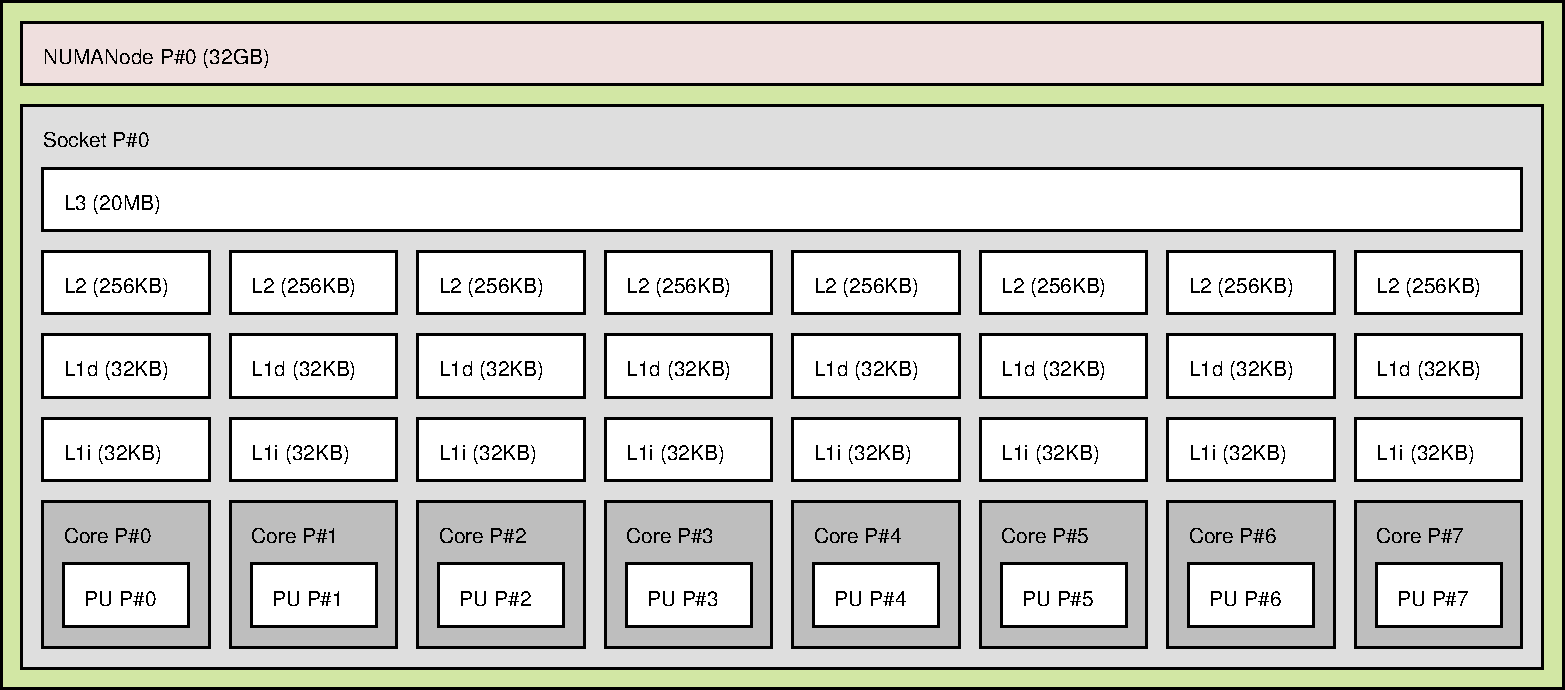
\includegraphics[width=0.8\textwidth]{figures/ada}
  \end{center}
    
\end{frame}

\begin{frame}{Experimental results: speedups}
  \begin{center}
    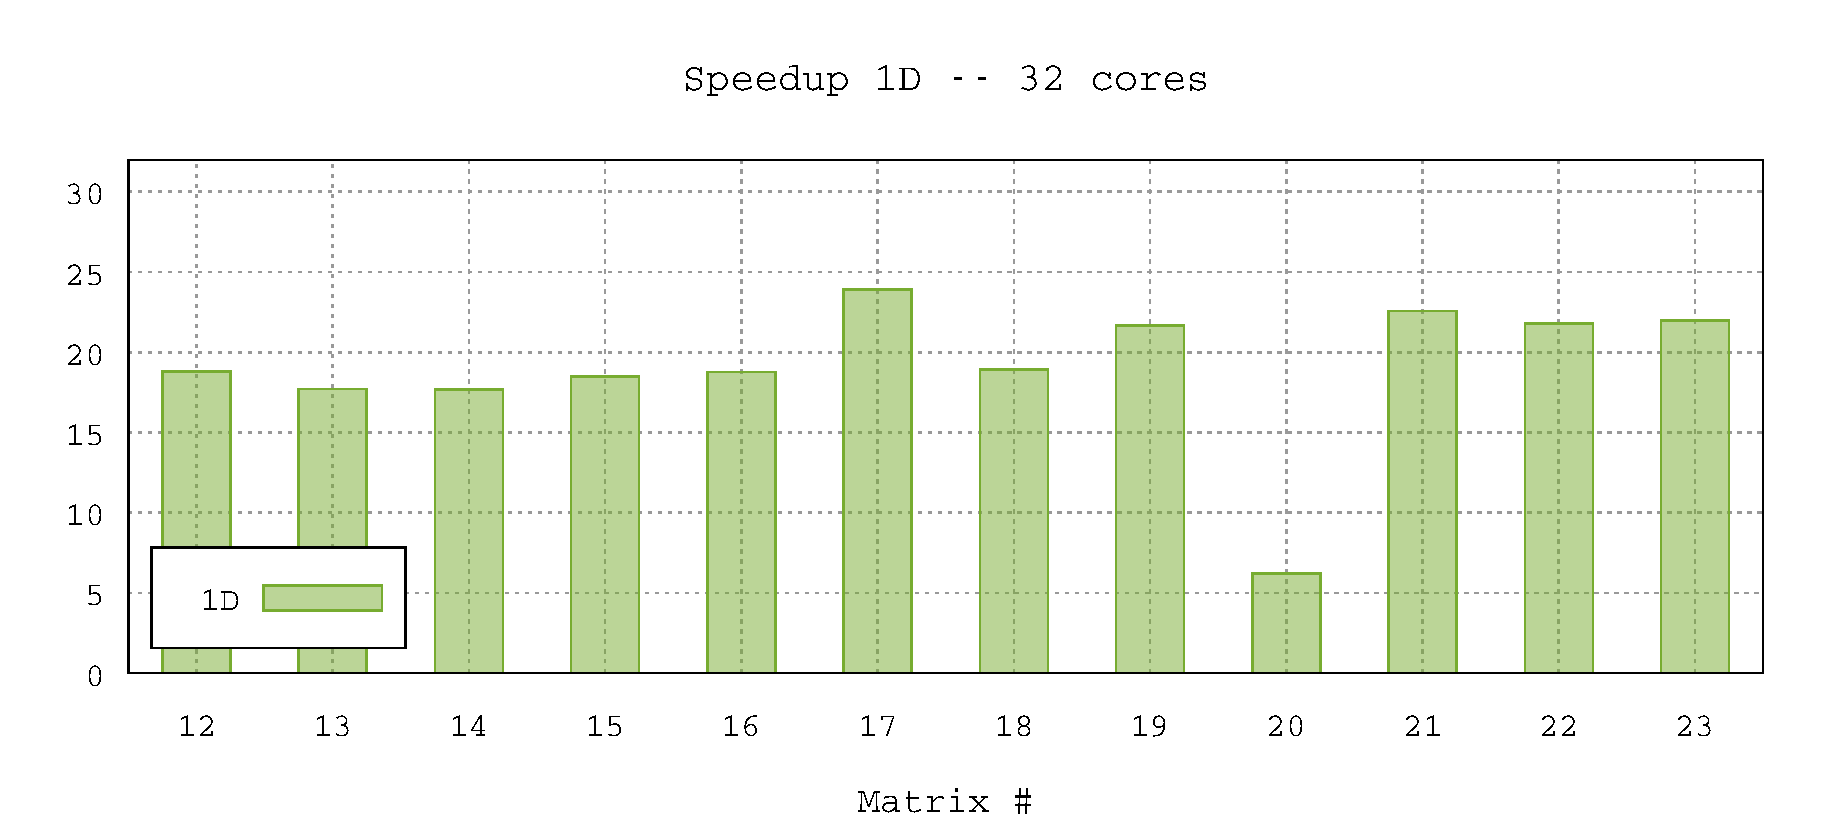
\includegraphics[width=0.9\textwidth]{data/su_ada_toms_1d}
  \end{center}
  
  The task-based multifrontal method, implemented with a STF parallel
  model on top of \starpu offers good speedups on 32 cores:

  \begin{itemize}
  \item speedup increases with problem size with very low speedup for
    some problem such as matrix \# 20
  \item we use a detailed performance analysis to determine the
    limiting factors of the STF 1D approach
  \end{itemize}

\end{frame}

\begin{frame}{Area performance upper bound}


  \begin{block}{Parallel efficiency}
    The \dr{parallel efficiency} is defined as
    
    \begin{displaymath}
      e(p) = \frac{\tilde{t}(1)}{t(p)\cdot p}
    \end{displaymath}
    
    \begin{itemize}
    \item $\tilde{t}(1)$ is the execution time of the \alert{best
        sequential algorithm} on one core;
    \item $t(p)$ is the execution time of the \alert{best parallel
        algorithm} on $p$ cores.
    \end{itemize}
  \end{block}
    
    \vspace{0.2cm}
    
  Note that, in general, $t(1) \ge \tilde{t}(1)$ because:
  \begin{itemize}
  \item parallelism requires partitioning of data and operations which
    reduces the efficiency of tasks;
  \item the parallel algorithm may trade some extra flops for
    concurrency.
  \end{itemize}


\end{frame}


% \begin{frame}{Area performance upper bound}

%   The \dr{parallel efficiency} can be defined as

%   \begin{displaymath}
%     e(p) = \frac{t^{min}(p)}{t(p)}
%   \end{displaymath}

%   where \dr{$t^{min}(p)$} is a lower bound on execution time on $p$  resources:
%   % resources corresponding to the \alert{best schedule} under the
%   % following assumptions:

%   % \begin{columns}
%   %   \begin{column}{0.45\textwidth}

%   %     \begin{enumerate}
%   %     \item<2-> No runtime overhead.
%   %     \item<3-> No tasks dependencies.
%   %     \item<4-> Tasks are moldable.
%   %       %% \item<2-> Tasks executed at asymptotic performance (\alert{maximum task granularity})
%   %       %% \item<2-> \alert{Perfect data locality}
%   %     \end{enumerate}

%   %   \end{column}
%   %   \begin{column}{0.55\textwidth}

%   %     \begin{center}
%   %       \only<1 >{\includegraphics[width=\textwidth]{lp_anim_mul2}}%
%   %       \only<2 >{\includegraphics[width=\textwidth]{lp_anim_mul3}}%
%   %       \only<3 >{\includegraphics[width=\textwidth]{lp_anim_mul4}}%
%   %       \only<4->{\includegraphics[width=\textwidth]{lp_anim_mul5}}%
%   %     \end{center}

%   %   \end{column}
%   % \end{columns}
      
%   \begin{itemize}
%   \item<2-> In the multicore case (homogeneous) we have 

%     \begin{displaymath}
%       t^{min}(p) = \frac{t(1) }{ p }
%     \end{displaymath}

%   \item<3-> We consider \dr{$t^{min}(p)$} when there is no performance
%     loss resulting from the parallelization
%     \dr{$\tilde{t}^{min}(p)$}. In the multicore case we have
    
%     \begin{displaymath}
%       \tilde{t}^{min}(p) = \frac{ \tilde{t}(1) }{ p }
%     \end{displaymath}

%   \end{itemize}

% \end{frame}


\begin{frame}{A finer performance analysis}
  The execution time $t(p)$ can be decomposed in the following three
  terms:
  \begin{itemize}
  \item \db{$t_t(p)$}: the time spent executing tasks.
  \item \mye{$t_r(p)$}: the overhead of the runtime system. \alert{$t_r(1):=0$}.
  \item \dg{$t_i(p)$}: idle time. \alert{$t_i(1):=0$}.
  \end{itemize}

  The overall efficiency can thus be written as:
  

  % \begin{displaymath}
    % e(p) = \frac{ \tilde{t}_t(1) }{ t_t(p) + t_r(p) + t_i(p) }
  % \end{displaymath}
  
  % \begin{displaymath}
    % = \mre{\overbracket{\mbk{\frac{ \tilde{t}_t(1) }{ t_t(1) }}}^{e_g}}\cdot 
    % \mbl{\overbracket{\mbk{\frac{ t_t(1) }{ t_t(p) }}}^{e_{t}}}\cdot  
    % \mgr{\overbracket{\mbk{\frac{ t_t(p) }{ t_t(p)+t_r(p) }}}^{e_r}}\cdot
    % \mye{\overbracket{\mbk{\frac{ t_t(p)+t_r(p)+ t_c(p) }{ t_t(p) + t_r(p) + t_c(p) + t_i(p) }}}^{e_p}}.
  % \end{displaymath}
  


\begin{align*}
  e(p) & = \frac{ \tilde{t}_t(1) }{ t_t(p) + t_r(p) + t_i(p) } \\
       & = \mre{\overbracket{\mbk{\frac{ \tilde{t}_t(1) }{ t_t(1) }}}^{e_g}}\cdot 
  \mbl{\overbracket{\mbk{\frac{ t_t(1) }{ t_t(p) }}}^{e_{t}}}\cdot  
  \mye{\overbracket{\mbk{\frac{ t_t(p) }{ t_t(p)+t_r(p) }}}^{e_r}}\cdot
  \mgr{\overbracket{\mbk{\frac{ t_t(p)+t_r(p)+ t_c(p) }{ t_t(p) + t_r(p) + t_c(p) + t_i(p) }}}^{e_p}}.
\end{align*}

    % \begin{displaymath}
    %   \tiny
    %     e(p) = \mbk{\frac{\tilde{t}^{area}(p)}{t(p)}} 
    %     % = \frac{ \tilde{t}^{area}(p) \times p }{ t_t(p) + t_r(p) + t_c(p) + t_i(p) } = \frac{ \tilde{t}^{area}_t(p) }{ t_t(p) + t_r(p) + t_c(p) + t_i(p) }
    %     = \mre{\overbracket{\mbk{\frac{ \tilde{t}^{area}_t(p) }{ t^{area}_t(p) }}}^{e_g}}\cdot
    %     \mbl{\overbracket{\mbk{\frac{ t^{area}_t(p) }{ t_t(p) }}}^{e_{t}}}\cdot
    %     \mgr{\overbracket{\mbk{\frac{ t_t(p) }{ t_t(p)+t_r(p) }}}^{e_r}}\cdot
    %     \mbp{\overbracket{\mbk{\frac{ t_t(p)+t_r(p) }{t_t(p)+t_r(p)+ t_c(p)}}}^{e_c}}\cdot
    %     \mye{\overbracket{\mbk{\frac{ t_t(p)+t_r(p)+ t_c(p) }{ t_t(p) + t_r(p) + t_c(p) + t_i(p) }}}^{e_p}}.
    % \end{displaymath}

%   \begin{displaymath}
% e(p) = \frac{t^{area}(p)}{t(p)} =%
% \only<1,3,4,5>{\overbracket{\frac{t^{area}_t(p)}{t_t(p)}}^{e_h}}%
% \only<2>{\dr{\overbracket{\frac{t^{area}_t(p)}{t_t(p)}}^{e_h}}}%
% \cdot%
% \only<1,2,4,5>{\overbracket{\frac{t_t(p)}{t_t(p)+t_r(p)}}^{e_r}}%
% \only<3>{\dg{\overbracket{\frac{t_t(p)}{t_t(p)+t_r(p)}}^{e_r}}}%
% \cdot%
% \only<1,2,3,5>{\overbracket{\frac{t_t(p)+t_r(p)}{t_t(p)+t_r(p)+t_i(p)}}^{e_p}}%
% \only<4>{\db{\overbracket{\frac{t_t(p)+t_r(p)}{t_t(p)+t_r(p)+t_i(p)}}^{e_p}}}%
%   \end{displaymath}
  
  \vspace{0.5cm}

  with:

  \vspace{0.3cm}

  \begin{overlayarea}{\textwidth}{3cm}
    \only<2>{\dr{$e_g$}: the \dr{granularity efficiency}. Measures the
      impact exploiting of parallel algorithms compared to sequential
      ones.}%
    \only<3>{\db{$e_t$}: the \db{task efficiency}. Measures the
      exploitation of data locality.}%
    \only<4>{\mye{$e_r$}: the \mye{runtime efficiency}. Measures how the
      runtime overhead affects performance.}%
    \only<5>{\dg{$e_p$}: the \dg{pipeline efficiency}. Measures how
      much concurrency is available and how well it is exploited.}%
    % \begin{itemize}
    % \item<5> if $e_h>1$ GPUs are overloaded and CPU starve ($e_p<1$)
    % \item<5> if $e_h<1$ tasks acceleration factor not properly exploited
    % \end{itemize}%

    % \only<7>{$e_t \cdot e_p$ measures the quality of the scheduling
    % and is $\leq 1$.}
  \end{overlayarea}

\end{frame}

\begin{frame}{Experimental results: efficiency breakdown}
  \centering
  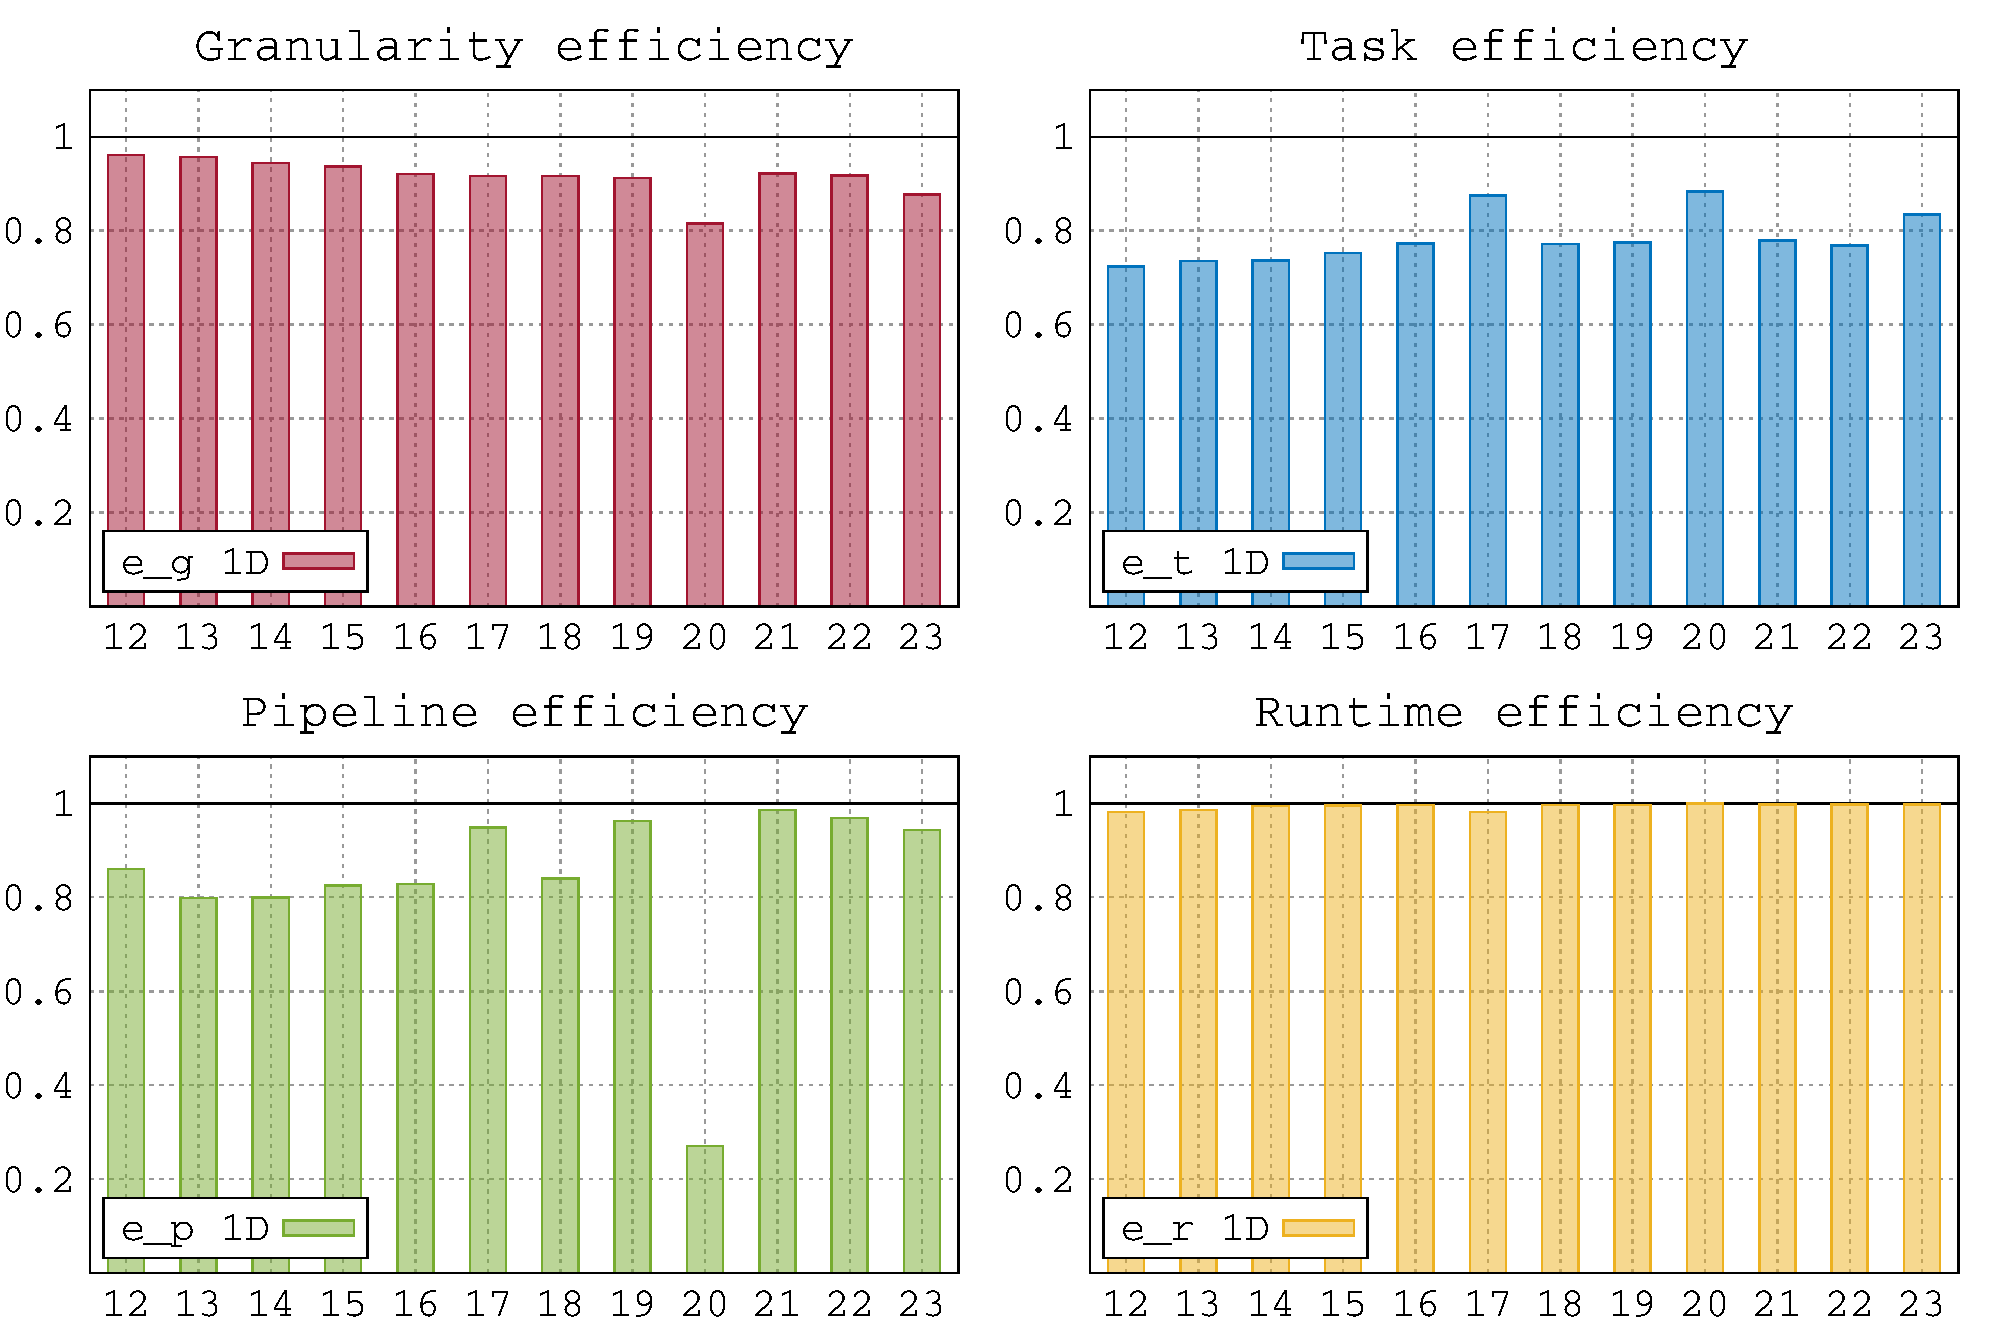
\includegraphics[width=\textwidth]{data/eff_profiles_2x2_1d}
\end{frame}

\begin{frame}{2D partitioning + CA front factorization}
  1D partitioning is not good for (strongly)
  \db{overdetermined} matrices:
  \begin{itemize}
  \item[\dr{$\blacktriangledown$}] Most fronts are overdetermined
  \item[\dg{$\blacktriangle$}] The problem is mitigated by
    concurrent front factorizations
  \end{itemize}


  \begin{columns}
    \begin{column}{0.8\textwidth}
      \begin{itemize}
      \item 2D block partitioning (not necessarily square)
        %% \item flat, binary (communication avoiding) or hybrid panel
        %%   reduction trees
      \item Communication avoiding algorithms
      \item[\dg{$\blacktriangle$}] More concurrency
      \item[\dr{$\blacktriangledown$}] More complex dependencies
      \item[\dr{$\blacktriangledown$}] Many more tasks (higher runtime overhead)
      \item[\dr{$\blacktriangledown$}] Finer task granularity (less kernel efficiency)
      \end{itemize}
      Thanks to the simplicity of the STF programming model it is
      possible to plug in \alert{2D methods} for factorizing the frontal
      matrices with a relatively moderate effort
    \end{column}
    \begin{column}{0.2\textwidth}
      \begin{center}
        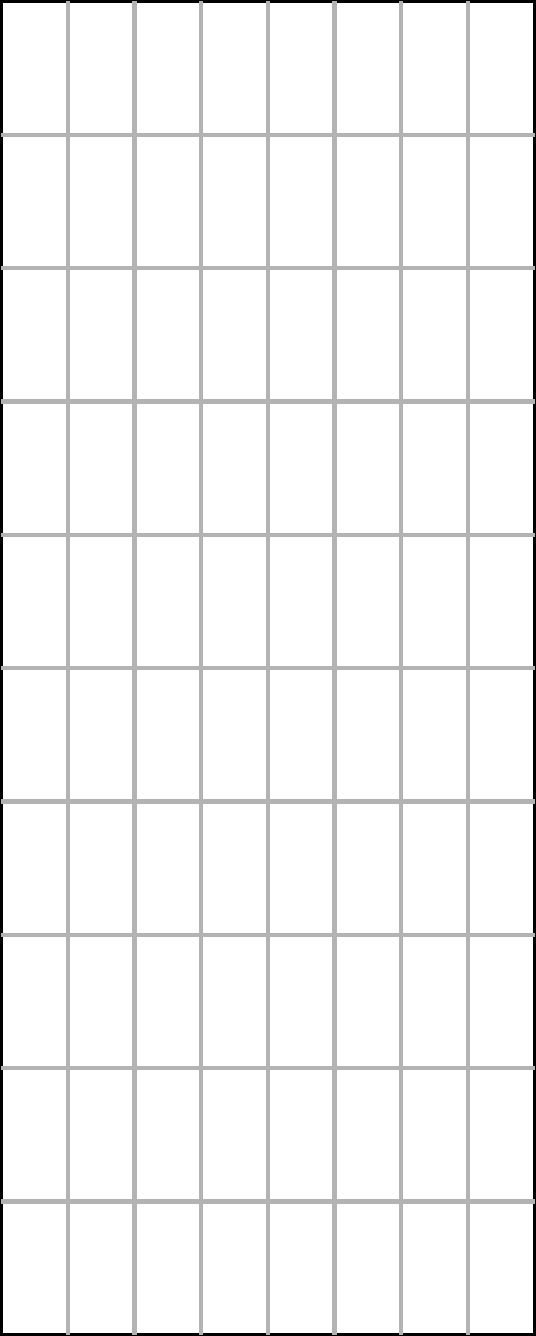
\includegraphics[width=\textwidth]{figures/2d}
      \end{center}
    \end{column}
  \end{columns}
\end{frame}

\begin{frame}[t,plain,fragile]{1D partitioning front factorization}
  \lstinputlisting{listings/mf-stf-multicore.f90}
\end{frame}

\begin{frame}[t,plain,fragile]{2D partitioning + CA front factorization}
  \lstinputlisting{listings/mf-stf-2d-multicore.f90}
\end{frame}

\begin{frame}{Experimental results: speedups}

  \begin{center}
    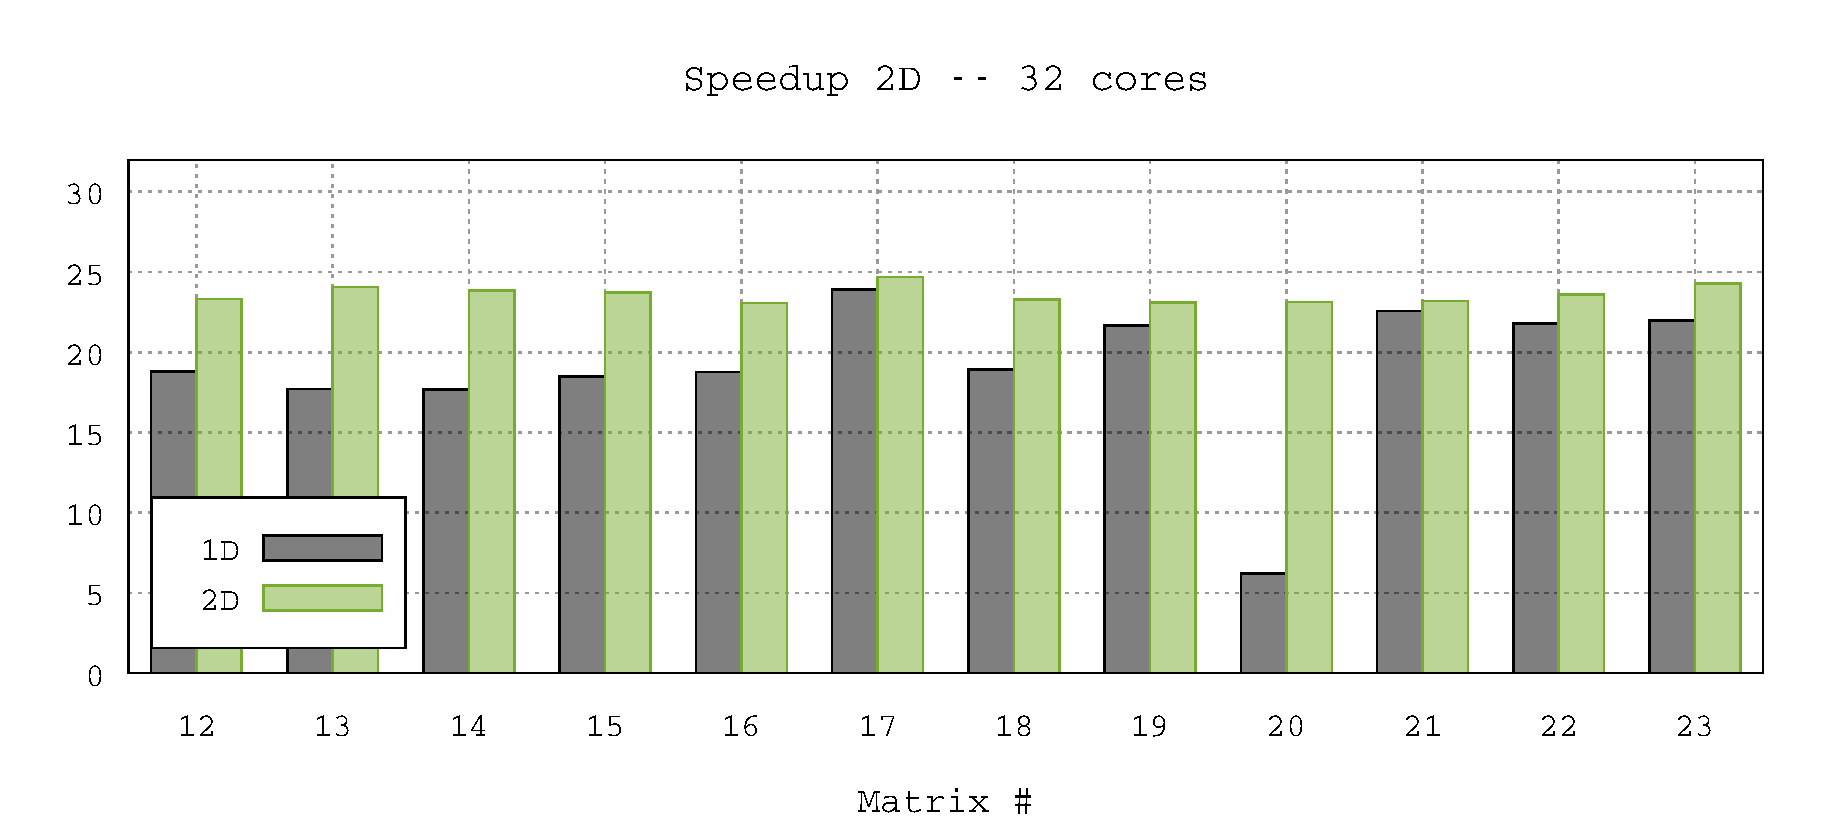
\includegraphics[width=0.9\textwidth]{data/su_ada_toms_2d}
  \end{center}

  The scalability of the task-based multifrontal method is enhanced by
  the the introduction of 2D CA algorithms:

  \begin{itemize}
  \item Speedups are \dr{uniform} for all tested matrices.
  \item We perform a comparative performance analysis wrt to the 1D
    case to show the benefits of the 2D scheme. 
  \end{itemize}

\end{frame}

\begin{frame}{Experimental results: efficiency breakdown}
  \centering
  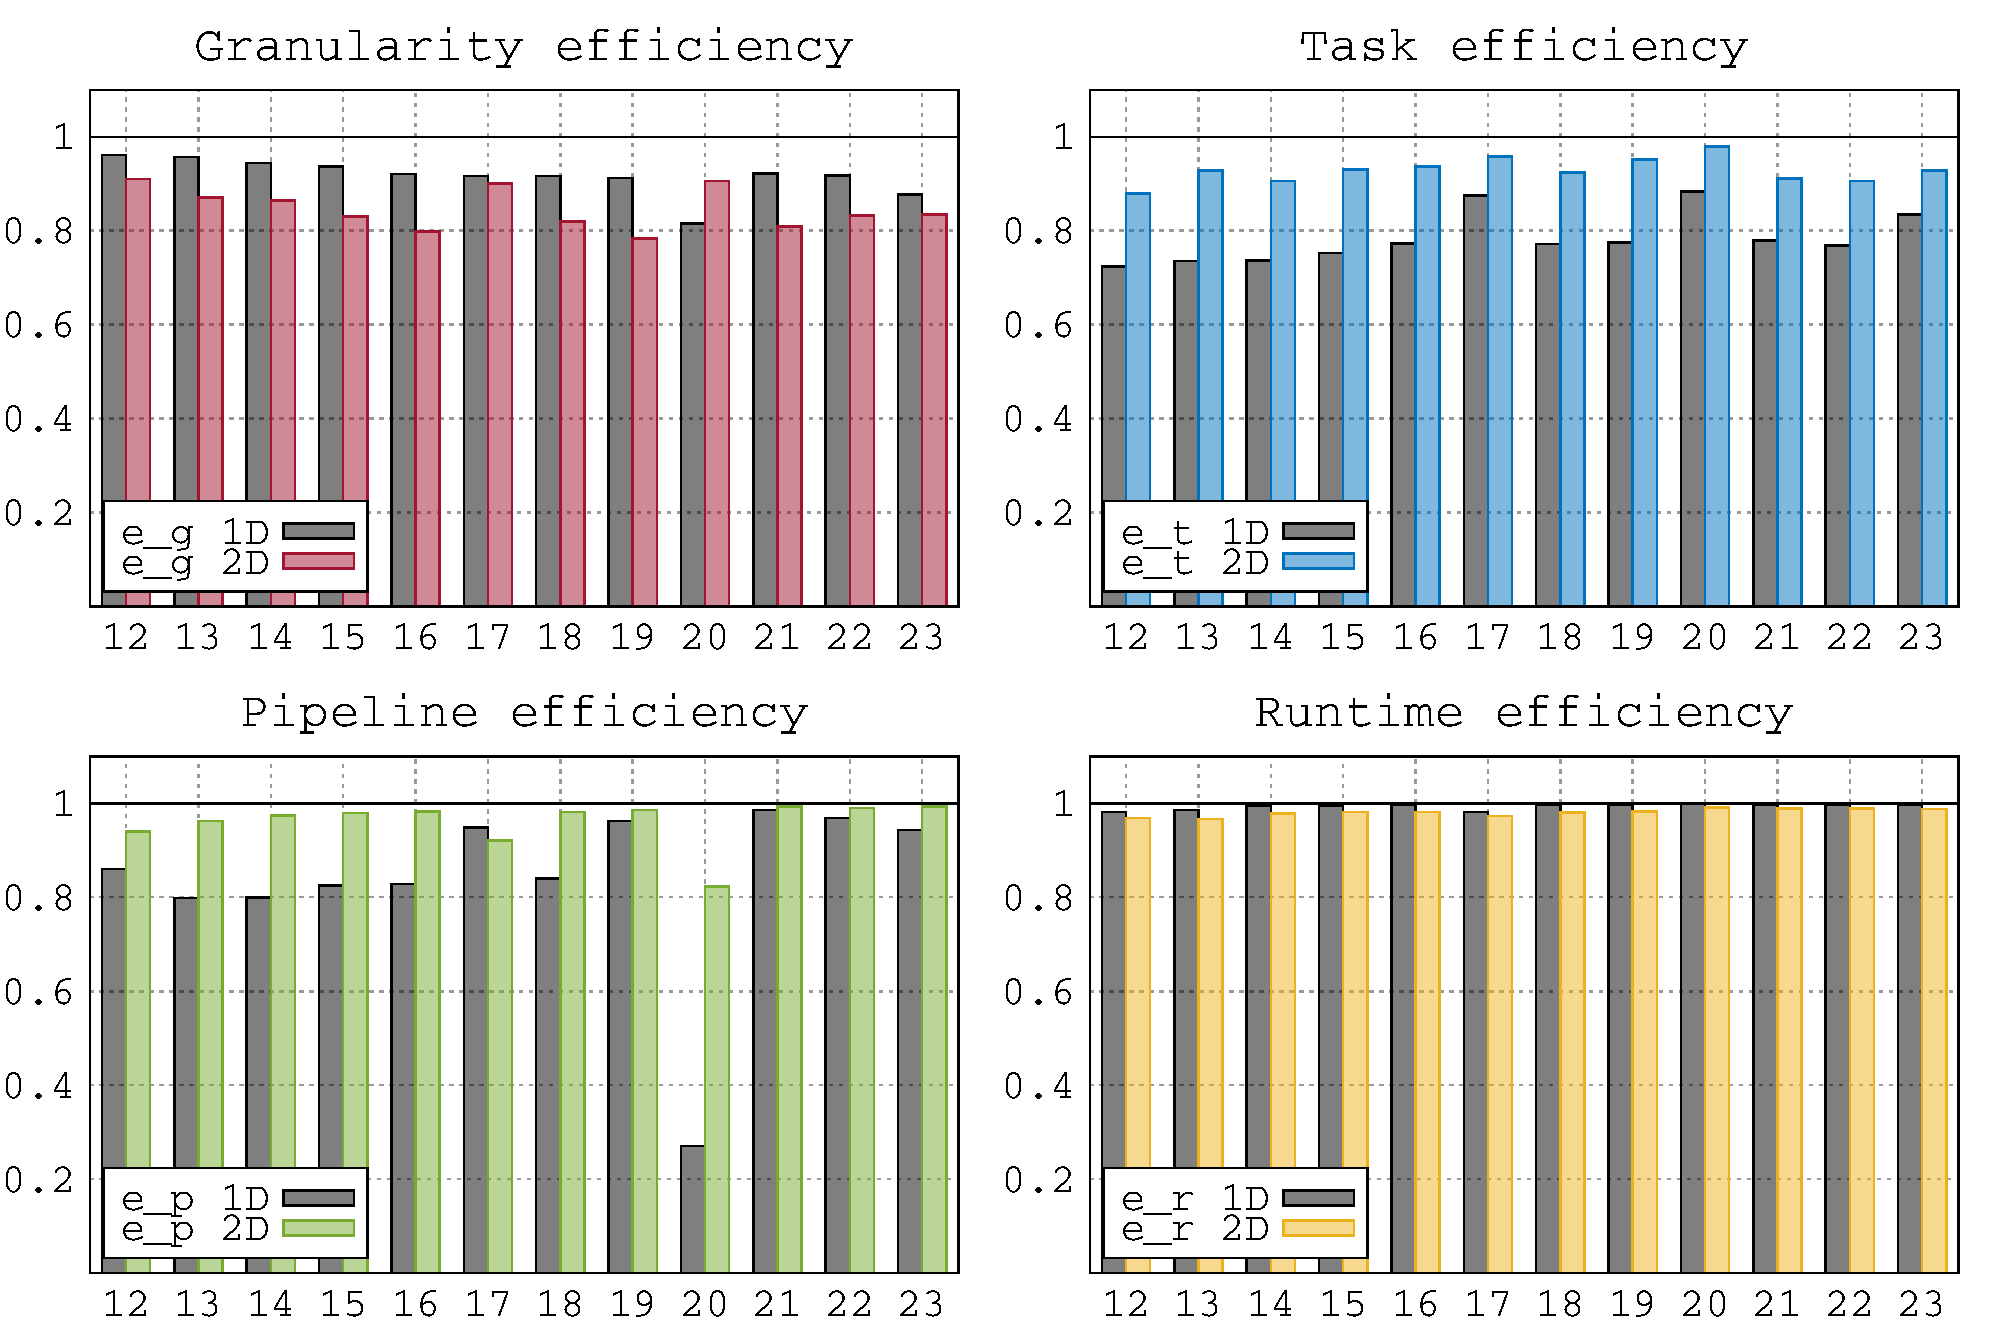
\includegraphics[width=\textwidth]{data/eff_profiles_2-2_2d}
\end{frame}

%%% Local Variables:
%%% mode: latex
%%% TeX-master: "defense"
%%% TeX-engine: xetex
%%% End:

\section{STF-based parallel multifrontal QR method for heterogeneous architectures}
\begin{frame}[plain]{GPU-based systems}
  
  % \begin{itemize}
  % \item[\dg{$\blacktriangle$}] 5x more floating-point performance than CPUs
    %% \item[\db{$\blacktriangle$}] Energy efficient

  \vspace{-0.8cm}

  % \item[\dr{$\blacktriangledown$}] Efficient on computationally
    % intensive kernels.
  % \item[\dr{$\blacktriangledown$}] Requires large granularity tasks to
    % feed GPUs resources.
  % \item[\dr{$\blacktriangledown$}] Memory transfers generally costly.
  % \end{itemize}  
  
  \begin{columns}
    \begin{column}{0.72\textwidth}
      \begin{itemize}
      \item Very high computing power ($O(1)$ Tflop/s)
      \item Very high memory bandwidth ($O(100)$ GB/s)
      \item Very convenient Gflops/s/Watt ratio ($O(10)$)  
      \end{itemize}
    \end{column}
    \begin{column}{0.28\textwidth}
      \begin{center}
        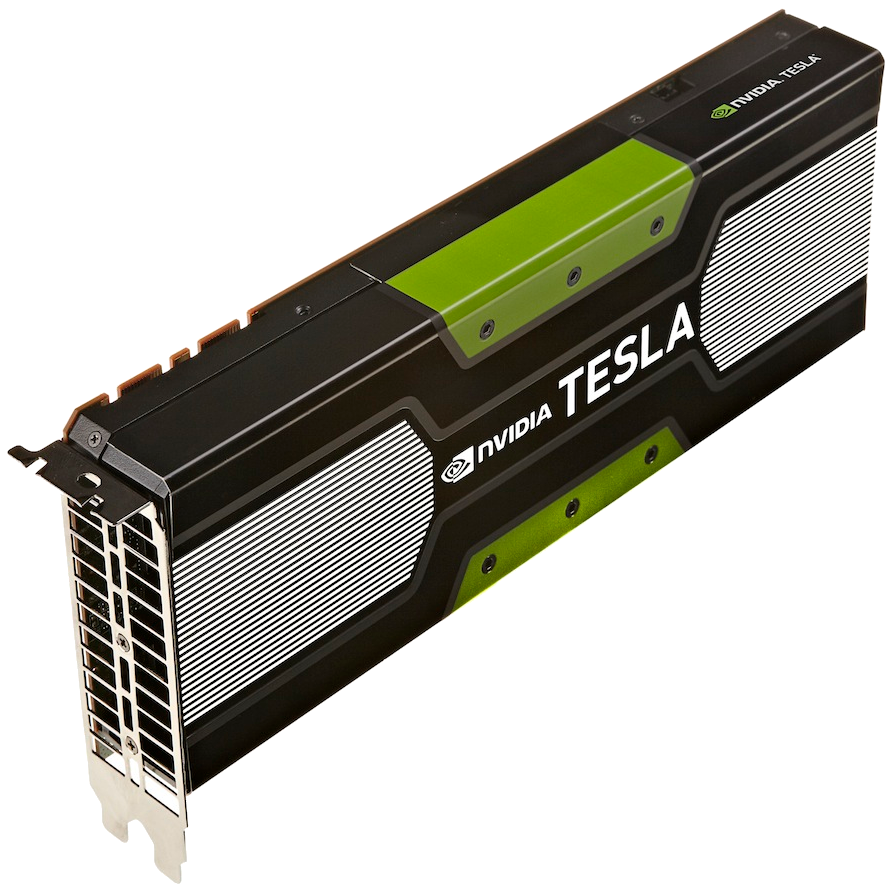
\includegraphics[width=0.9\textwidth]{figures/tesla.png}
      \end{center}
    \end{column}
  \end{columns}
  

  \begin{block}{Objective}
    Exploit \dr{heterogeneity} (i.e. take advantage of the diversity of
    resources) to accelerate the multifrontal QR factorization.
  \end{block}

  \vspace{0.2cm}

  \uncover<2->{
  % \begin{exampleblock}{Challenges}
    Issues:
    \begin{itemize}
    \item<2-> \alert{Granularity}: GPUs require coarser grained tasks to
      achieve full speed;
    \item<3-> \dg{Scheduling}: account for different computing
      capabilities and different tasks characteristics while
      maximizing concurrency;
    \item<4> \db{Communications}: minimize the cost of host-to-device
      data transfers.
    \end{itemize}  
  % \end{exampleblock}
}

\end{frame}

% \begin{frame}[fragile,t]{The multifrontal QR factorization: GPU-based systems}

% STF parallel \qrm code

% \begin{lstlisting}[basicstyle=\tt\tiny, escapechar=|]
% do f=1, nfronts ! in postorder
%    ! compute structure and register handles
%    call activate(f)
%    ! allocate and initialize front
%    call submit(init, f:RW)

%    do c=1, f%nc ! for all the children of f
%       do j=1,c%n
%          ! assemble column j of c into f
%          call submit(assemble, c(j):R, f:RW)
%       end do
%       ! Deactivate child
%       call submit(deactivate, c:RW)
%    end do

%    do p=1, f%n
%       ! panel reduction of column p
%       call submit(_geqrt, f(p):RW)
%       do u=p+1, f%n
%          ! update of column u with panel p
%          call submit(_gemqrt, f(p):R, f(u):RW)
%       end do
%    end do
% end do
% ! wait for the tasks to be executed
% call wait_tasks_completion()
% \end{lstlisting}
% \end{frame}


% \begin{frame}[fragile,t]{The multifrontal QR factorization: GPU-based systems}

% STF parallel \qrm code

% \begin{lstlisting}[basicstyle=\tt\tiny, escapechar=|]
% do f=1, nfronts ! in postorder
%    ! compute structure and register handles
%    call activate(f)
%    ! allocate and initialize front
%    call submit(init, f:RW)

%    do c=1, f%nc ! for all the children of f
%       do j=1,c%n
%          ! assemble column j of c into f
%          call submit(assemble, c(j):R, f:RW)  |\alert{$\leftarrow$ CPU and GPU task}|
%       end do
%       ! Deactivate child
%       call submit(deactivate, c:RW)
%    end do

%    do p=1, f%n
%       ! panel reduction of column p
%       call submit(_geqrt, f(p):RW)             |\alert{$\leftarrow$ CPU and GPU task}|
%       do u=p+1, f%n
%          ! update of column u with panel p
%          call submit(_gemqrt, f(p):R, f(u):RW) |\alert{$\leftarrow$ CPU and GPU task}|
%       end do
%    end do
% end do
% ! wait for the tasks to be executed
% call wait_tasks_completion()
% \end{lstlisting}
% \end{frame}

\begin{frame}{Frontal matrices partitioning strategies}
  \begin{columns}    
    \begin{column}{0.7\textwidth}
      %Front partitioning:
      \begin{itemize}
      % \item<1->\dg{Fine grain}~\citet{b:12}, ~\alert{\PaperPortrait\cite{a.b.g.l.:13,a.b.g.l.:14}}
      \item<1->\dg{Fine grain} (e.g., \texttt{qr\_mumps})
        \begin{itemize}
        \item<2->[\dg{$\blacktriangle$}]     high concurrency.
        \item<2->[\dr{$\blacktriangledown$}] low tasks efficiency.
        \end{itemize}
      \end{itemize}
      \begin{itemize}
      % \item<3->\db{Coarse grain} MAGMA library by~\citet{a.d.d.h.ea:09}

      \item<3->\db{Coarse grain} (e.g., MAGMA by Agullo et al.)

        \vspace{-0.2cm}

        \begin{itemize}
        \item<4->[\dg{$\blacktriangle$}]     optimum granularity for GPU. 
        \item<4->[\dr{$\blacktriangledown$}] limited concurrency. % and lookahead
        \end{itemize}
      \end{itemize}
      % \begin{itemize}
      % \item<5->\dr{Hierarchical}
      %   \begin{itemize}
      %   \item<7->[\dg{$\blacktriangle$}]  granularity and concurrency trade-off. 
      %   \item<7->[\dg{$\blacktriangle$}]  heterogeneity to be exploited.
      %   \item<8> requires \alert{dynamic repartitioning}.
      %   % \item<8> requires clever \alert{scheduling} to execute a
      %   %   heterogeneous workload on a heterogeneous machine

      %   \end{itemize}
      % \end{itemize}
      % \begin{block}<5->{Hierarchical ~~\PaperPortrait\cite{a.b.g.l.:15}}

      \vspace{0.3cm}

      \begin{block}<5->{Hierarchical}
        \begin{itemize}
        \item<7->[\dg{$\blacktriangle$}]  granularity and concurrency trade-off. 
        \item<7->[\dg{$\blacktriangle$}]  heterogeneity to be exploited.
        \item<8> requires \alert{dynamic repartitioning}.
        % \item<8> requires clever \alert{scheduling} to execute a
        %   heterogeneous workload on a heterogeneous machine

        \end{itemize}
      \end{block}

      % \begin{block}<1->{Fine grain}
      %   \begin{itemize}
      %   \item[\dg{$\blacktriangle$}]     high concurrency
      %   \item[\dr{$\blacktriangledown$}] low tasks efficiency
      %   \end{itemize}
      % \end{block}
      % \begin{block}<3->{Coarse grain (Magma)}
      %   \begin{itemize}
      %   \item[\dg{$\blacktriangle$}]     optimum granularity for GPU 
      %   \item[\dr{$\blacktriangledown$}] limited concurrency and lookahead
      %   \end{itemize}
      % \end{block}
      % \begin{block}<5->{Hierarchical}
      %   \begin{itemize}
      %   \item[\dg{$\blacktriangle$}]  granularity and concurrency trade-off 
      %   \item[\dg{$\blacktriangle$}]  heterogeneity to be exploited
      %   \end{itemize}
      % \end{block}
    \end{column}
    \begin{column}{0.3\textwidth}
      \begin{center}
        \only<1>{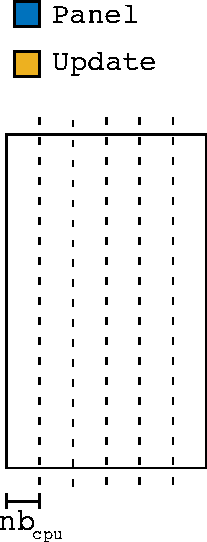
\includegraphics[width=0.8\textwidth]{figures/front_part_fine}}%
        \only<2>{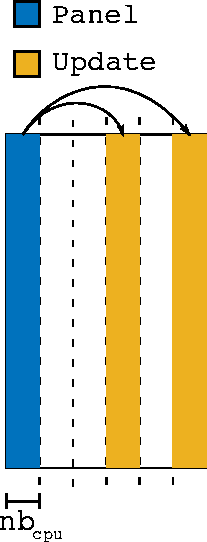
\includegraphics[width=0.8\textwidth]{figures/front_part_fine_ops}}%
        \only<3>{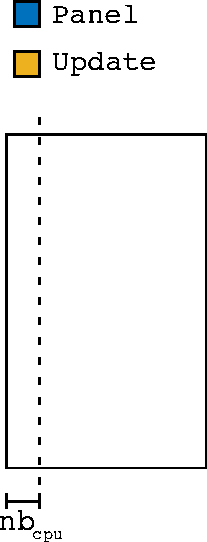
\includegraphics[width=0.8\textwidth]{figures/front_part_coarse}}%
        \only<4>{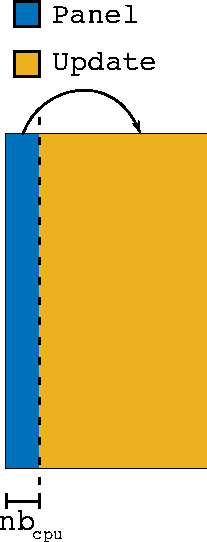
\includegraphics[width=0.8\textwidth]{figures/front_part_coarse_ops}}%
        \only<5>{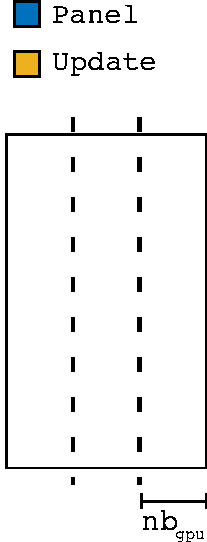
\includegraphics[width=0.8\textwidth]{figures/front_part_hier}}%
        \only<6>{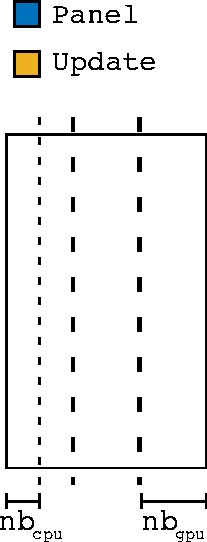
\includegraphics[width=0.8\textwidth]{figures/front_part_hier_repart}}%
        \only<7->{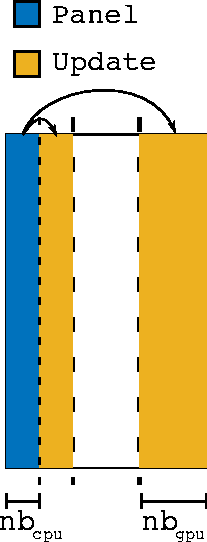
\includegraphics[width=0.8\textwidth]{figures/front_part_hier_ops}}
      \end{center}
    \end{column}
  \end{columns}
\end{frame}

\begin{frame}[fragile]{Frontal matrices partitioning strategies}

% The partitioning is achieved \alert{dynamically} through a
% partitioning task:

\begin{itemize}
% \item the partitioning is dynamic
\item The partitioning is done \alert{dynamically} through a
  \alert{partitioning task}.
\item the partitioning is \alert{symbolic}: neither allocations nor data
  copies.
\item the runtime ensures the \alert{consistency} of data.
\end{itemize}
  
\vspace{0.5cm}

\lstinputlisting[escapechar=|]{listings/hierarchical.f90}


% \begin{lstlisting}[basicstyle=\tt\tiny]
% forall outer panels o_p=1...o_n in f
%    ! partition (outer) block column f(o_p) into
%    ! i_n inner block columns f(o_p,1) .. f(o_p,i_n)
%    call submit(partition, f(o_p):R, f(o_p,1):RW, .., f(o_p,i_n):RW)

%    forall inner panels i_p=1..i_n
%       ! panel reduction of inner block column i_p
%       call submit(inner_panel, f(i_p):RW)
%       forall inner blockcolumns i_u=i_p+1..i_n in f(o_p)
%         ! update (inner) column in_u with panel p
%         call submit(inner_update, f(i_p):R, f(i_u):RW)
%       end do
%    end do

%    forall outer blockcolumns o_u=o_p+1..o_n
%       forall inner panels i_p=1..in_n
%        ! update outer block column o_u with panel i_p
%          call submit(outer_update, f(i_p):R,f(o_u):RW)
%       end do
%    end do     

%    ! unpartition (outer) block column
%    call submit(unpartition, f(o_p,1):R..f(o_p,i_n):R, f(o_p):RW)
% end do
%   \end{lstlisting}

\end{frame}

\begin{frame}{Tasks scheduling for heterogeneous architecture}

  % Multiple sources of heterogeneity:

  % \begin{columns}
  %   \begin{column}{0.5\textwidth}

  \begin{block}{Workload heterogeneity}
    \begin{itemize}
    \item \alert{Hierarchical partitioning}: fine and coarse
      granularity tasks.
    \item \alert{Variability of front sizes}: variation of tasks
      granularity.
    \item \dr{Compute-bound} and \dr{memory-bound} tasks.
    \end{itemize}    
  \end{block}

  % \end{column}
  % \begin{column}{0.5\textwidth}

  \begin{block}{Architecture heterogeneity}
    \begin{itemize}
    \item \dr{Processor} speeds and capabilities.
    \item \dr{Memory} speeds and transfers.
    \end{itemize}
  \end{block}

  % \end{column}
  % \end{columns}

  % \begin{itemize}
  %   \item Workload heterogeneity:
  %     \begin{itemize}
  %     \item The \alert{hierarchical partitioning} scheme produces fine and
  %       coarse granularity tasks.
  %     \item The \alert{variability of front sizes} in the etree induces a big
  %       variation of tasks granularity.
  %     \item Compute-bound and memory-bound tasks.
  %     \end{itemize}
  %   \item Architecture heterogeneity:
  %     \begin{itemize}
  %     \item Processor speeds.
  %     \item Memory speeds.
  %     \item Memory transfers.
  %     \end{itemize}
  % \end{itemize}

  \vspace{0.5cm}

  \dr{Multiple sources of heterogeneity}: Efficiently execute the task
  graph on the architecture requires a clever \alert{scheduling}
  strategy capable of taking into account resource capabilities.
 
\end{frame}

\begin{frame}[t]{Dynamic scheduling: building blocks}
  
  \vspace{-0.5cm}

  \begin{center}
    \only<1>{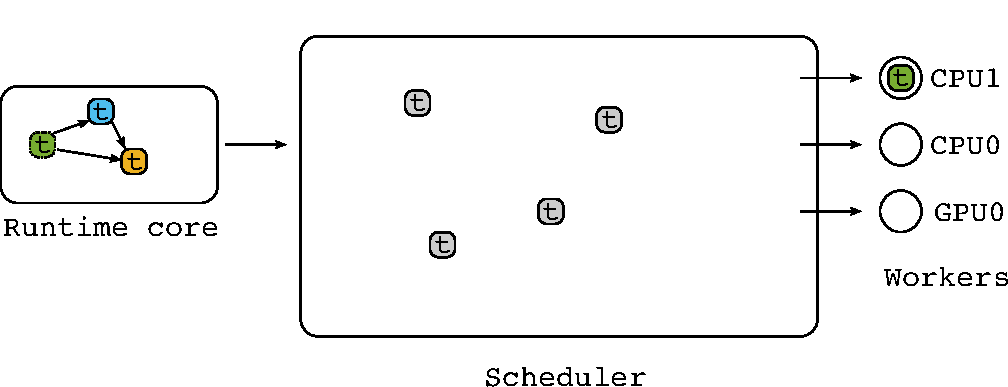
\includegraphics[width=0.8\textwidth]{figures/sched_running}}%
    \only<2>{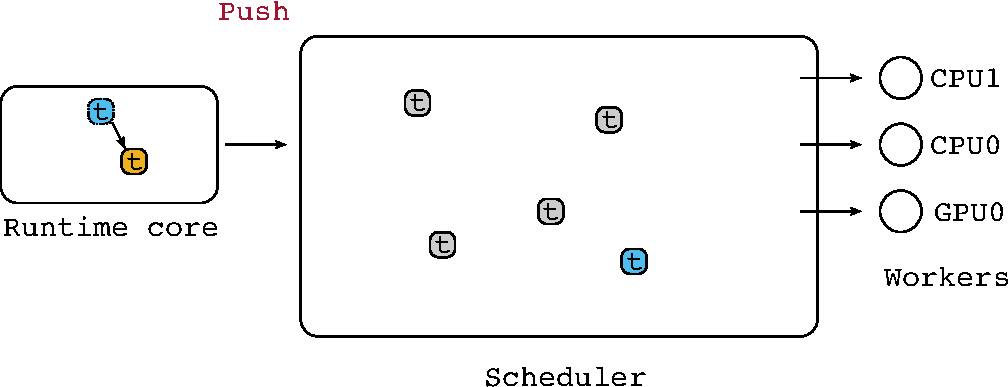
\includegraphics[width=0.8\textwidth]{figures/sched_push}}%
    \only<3>{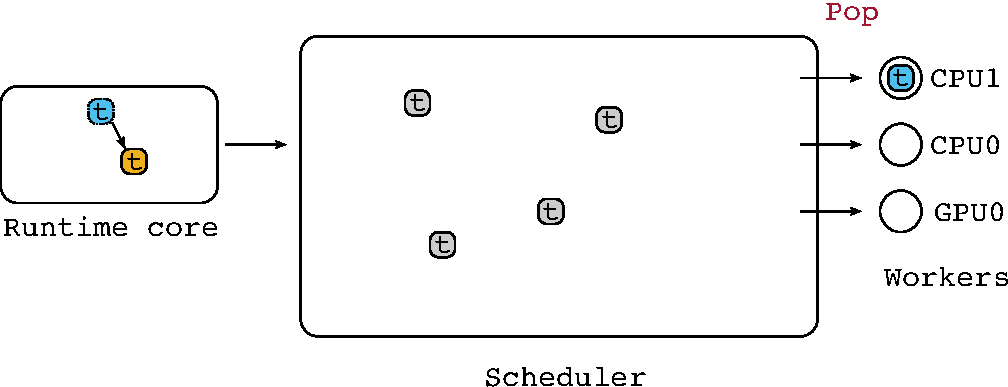
\includegraphics[width=0.8\textwidth]{figures/sched_pop}}%
    % \only<4-5>{\includegraphics[width=0.8\textwidth]{figures/sched_heft}}%
  \end{center}

  \vspace{-0.5cm}

  \begin{overlayarea}{\textwidth}{4cm}
    \only<1-3>{%
      \begin{block}{Building Blocks}
        \begin{itemize}
        \item A \dr{task container} storing tasks ready for execution.
        \item<2-3> Two methods:
          \begin{itemize}
          \item<2-3> \dr{{\tt push}}: put ready tasks in the scheduler.
          \item<3> \dr{{\tt pop }}: retrieve ready tasks from scheduler.
          \end{itemize}
        \end{itemize}
      \end{block}}%
    % \only<4-5>{%
    %   \begin{block}{DMDA (dynamic variant of HEFT~\cite{t.h.w:02})}
    %     \begin{itemize}
    %     \item<4-5> One queue per worker
    %     \item<4-5> Tasks are assigned at {\tt push} according to task priorities and a
    %       \alert{Minimum Completion Time} criterion
    %     \item[\dg{$\blacktriangle$}]<5> Data prefetching
    %     \item[\dr{$\blacktriangledown$}]<5> Runtime overhead: centralized and expensive 
    %     \item[\dr{$\blacktriangledown$}]<5> Local decision                              
    %     \end{itemize}
    %   \end{block}}%
  \end{overlayarea}
\end{frame}

\begin{frame}[t]{HeteroPrio scheduler}
  
  \vspace{-0.5cm}

  \begin{center}
    \only<1->{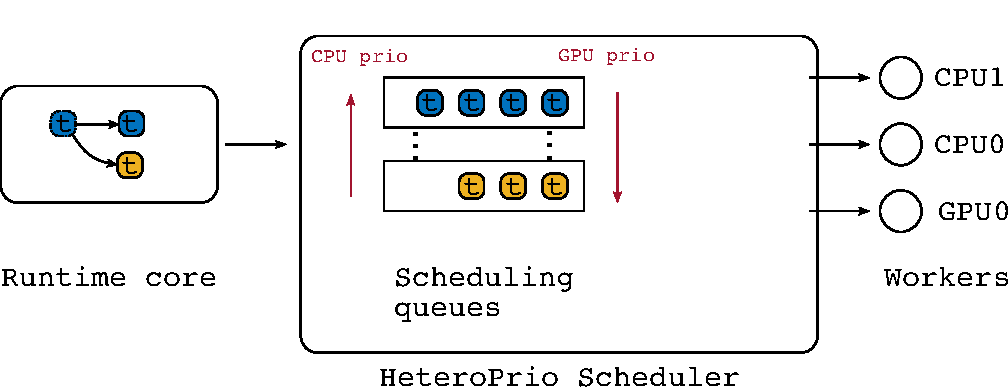
\includegraphics[width=0.8\textwidth]{figures/sched_hp}}%
  \end{center}

  \vspace{-0.5cm}

  \begin{block}{HeteroPrio}
    \begin{itemize}
    \item Introduced by Agullo \textit{et al.} for Fast Multipole Methods;
    \item Tasks are prioritized on each type of resources
      according to their \dr{acceleration factor}:
      \begin{enumerate}
      \item Performance ratio compared to other resources;
      \item Kernel efficiency.
      \end{enumerate}
    \item[\dg{$\blacktriangle$}]<2> Good matching between tasks
      and units.
    \end{itemize}
  \end{block}
\end{frame}

\begin{frame}[t]{HeteroPrio scheduler: extension 1/2}
  
  \vspace{-0.5cm}

  \begin{center}
    % \only<1>{\includegraphics[width=0.8\textwidth]{sched_hp_steady}}%
    \only<1->{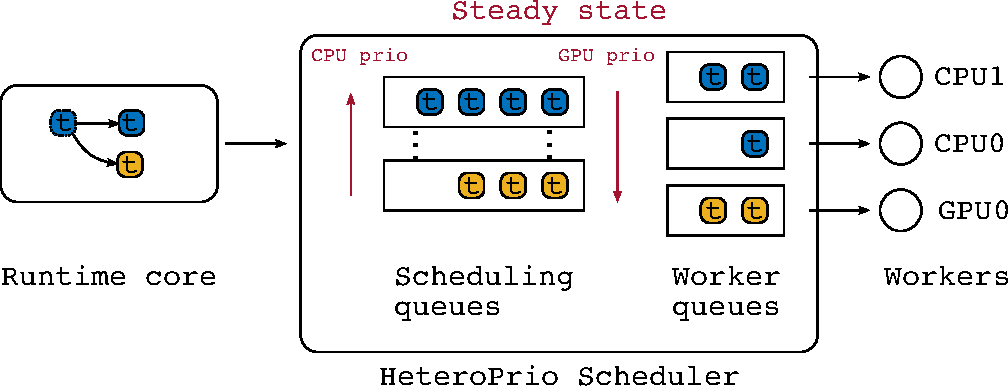
\includegraphics[width=0.8\textwidth]{figures/sched_hp_steady_wqueues}}%
  \end{center}

  \vspace{-0.5cm}

  \begin{overlayarea}{\textwidth}{4cm}
    \only<1-2>{%
      \begin{block}{HeteroPrio: data prefetching}
        \begin{itemize}
        \item Added one worker queue per worker;
        \item Tasks are put in scheduling queues at \dr{push}
          operation and moved to worker queues at \dr{pop};
        \item[\dg{$\blacktriangle$}]<2> Slightly anticipated task
          assignment: overlapped communication and computations.
        \end{itemize}
      \end{block}}%
  \end{overlayarea}
\end{frame}

\begin{frame}[t]{HeteroPrio scheduler: extension 2/2}

  % The scheduler HeteroPrio is introducted in~\citet{a.b.c.d.ea:14} in
  % the context of Fast Multipole methods.

  \begin{center}
    \only<1>{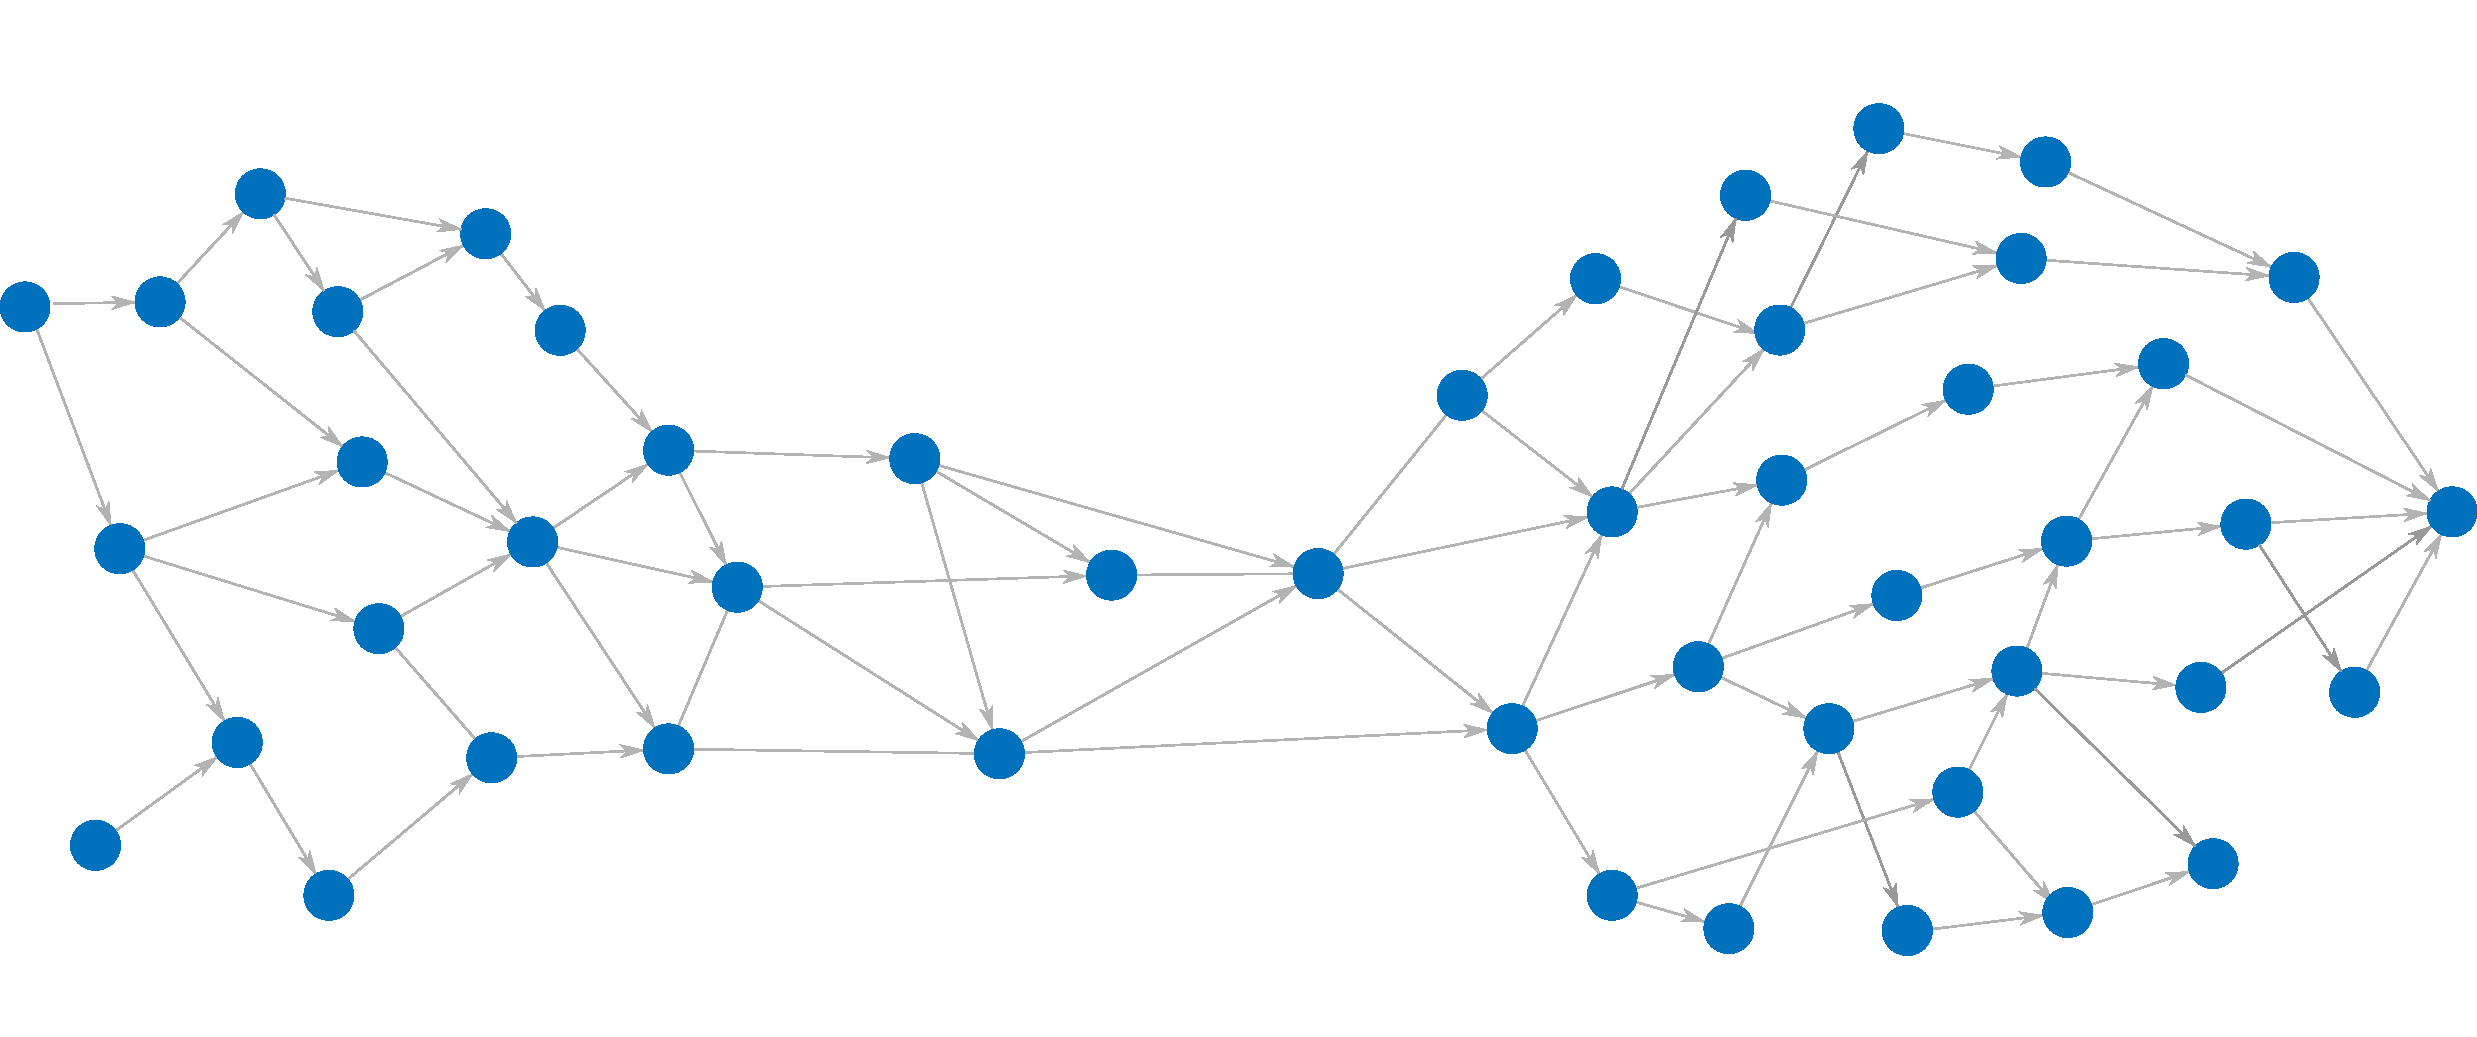
\includegraphics[width=0.8\textwidth]{figures/irregular_dag1}}%
    \only<2>{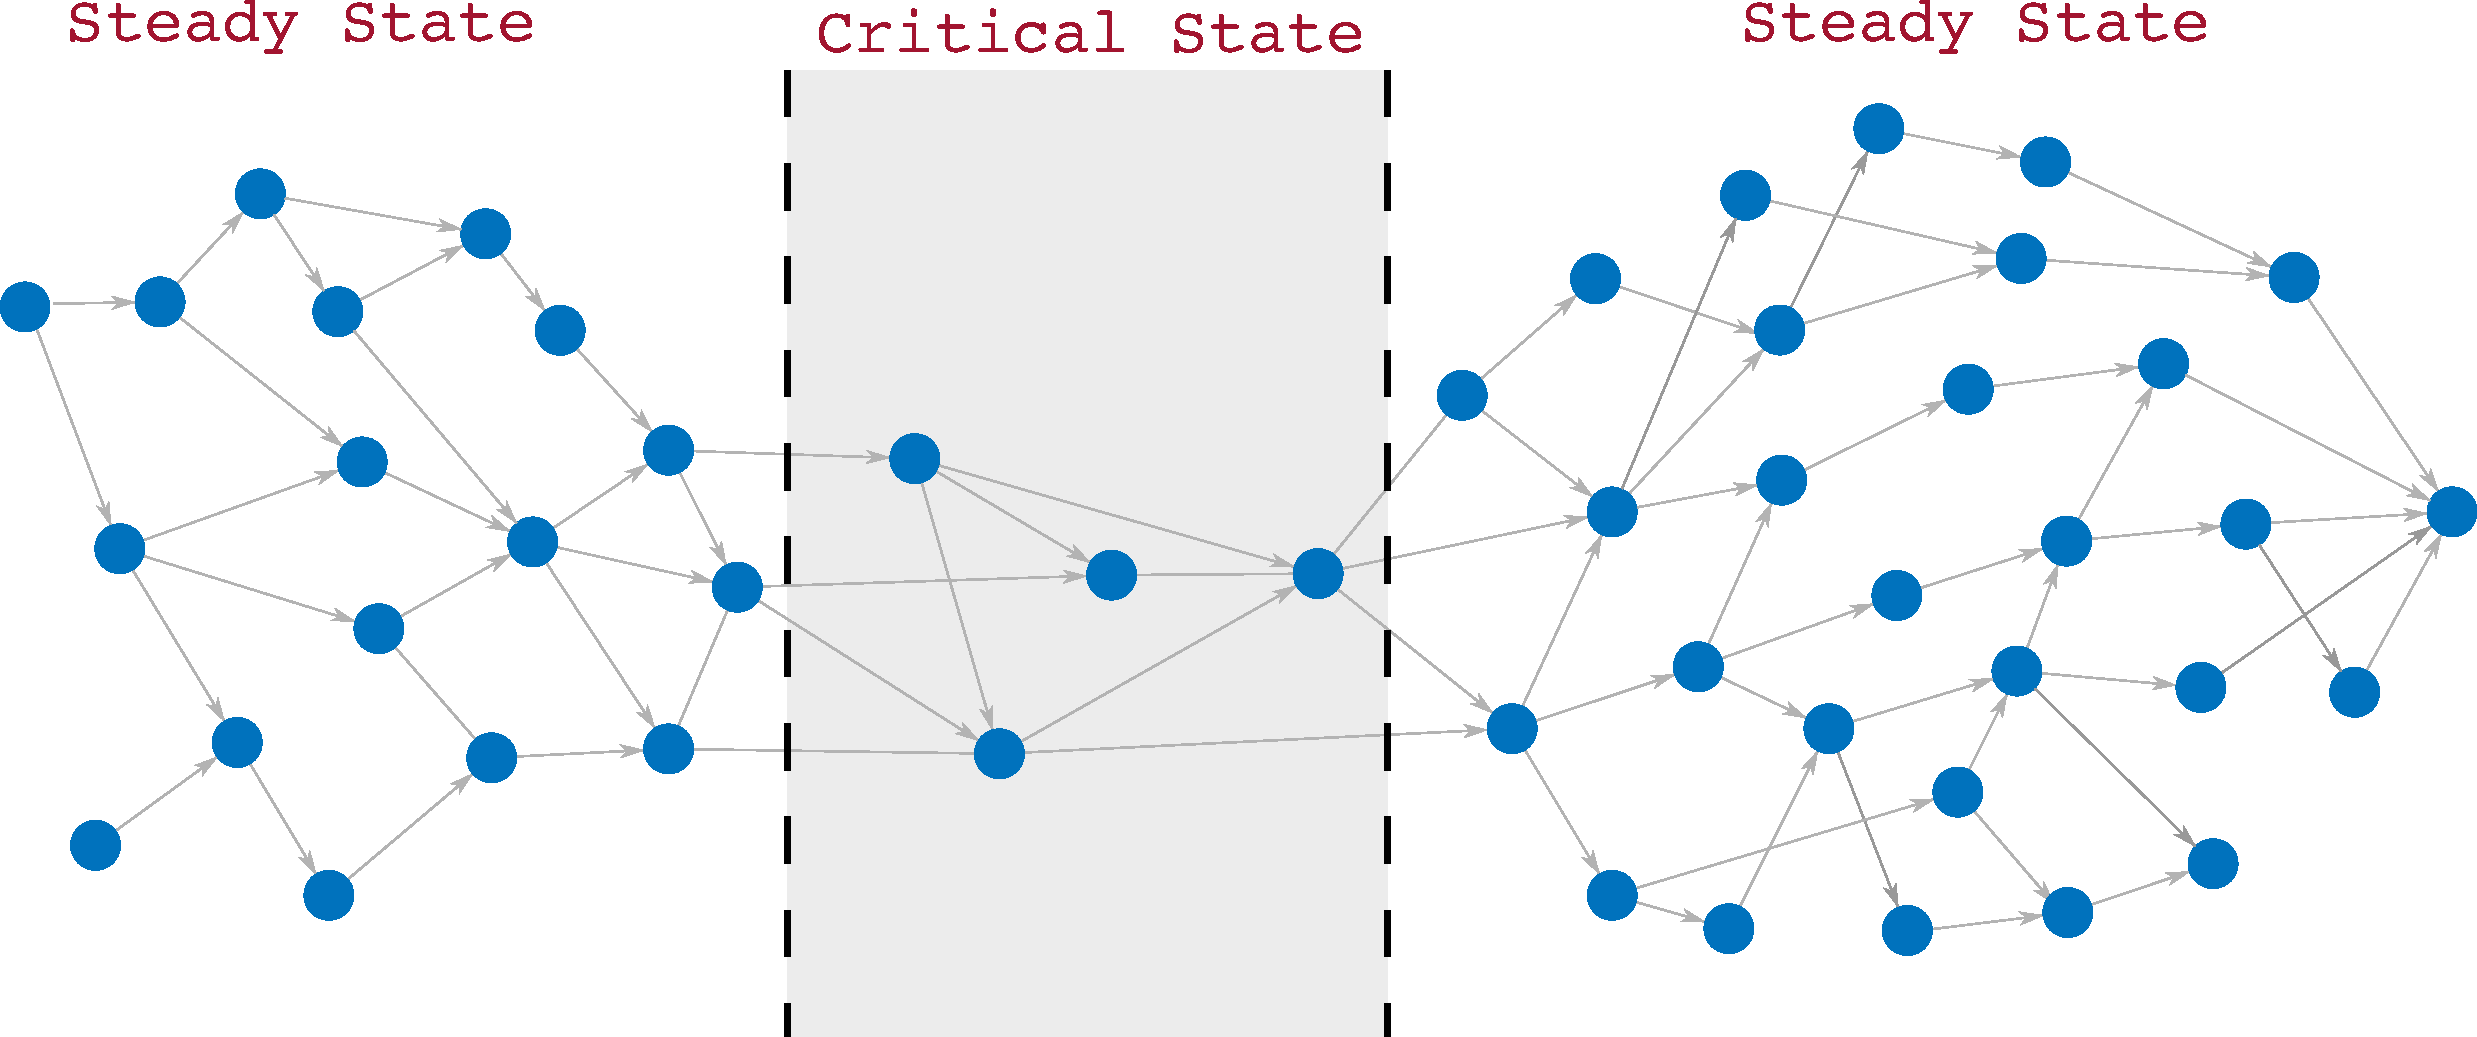
\includegraphics[width=0.8\textwidth]{figures/irregular_dag2}}%
  \end{center}

  % The parallel execution consists in a succession of two states:
  DAGs may be irregular and alternate rich and poor concurrency
  regions. \uncover<2>{
  Our scheduler switches automatically between two states:
  \begin{itemize}
  \item \db{Steady-state}: \# of ready tasks $>>$ number of resources:
    \alert{execute tasks where they are best suited} i.e. best
    acceleration factor.
  \item \db{Critical-state}: \# of ready tasks $<<$ number of resources:
    \alert{reduce the time spent on the critical path}.
  \end{itemize}}

  % \begin{center}
  %   \includegraphics[width=0.8\textwidth]{figures/steady_critical}
  % \end{center}

  % We use two set of queues: scheduling and worker queues and
  % scheduling decisions are taken at \alert{ {\tt pop}} operation:
  % \begin{itemize}
  % \item Pull a task form worker queue.
  % \item Fill worker queue retrieving tasks from scheduling queue.
  % \end{itemize}
\end{frame}

\begin{frame}[t]{HeteroPrio scheduler: extension 2/2}
    
  \begin{center}
    \only<1>{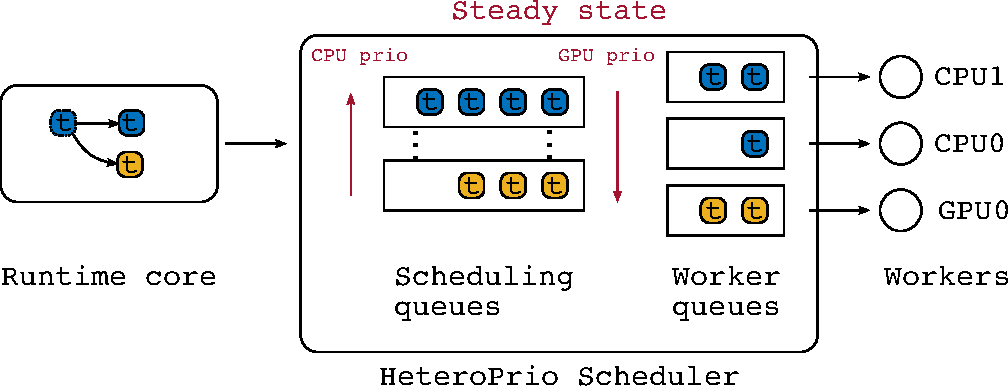
\includegraphics[width=0.8\textwidth]{figures/sched_hp_steady_wqueues}}%
    \only<2->{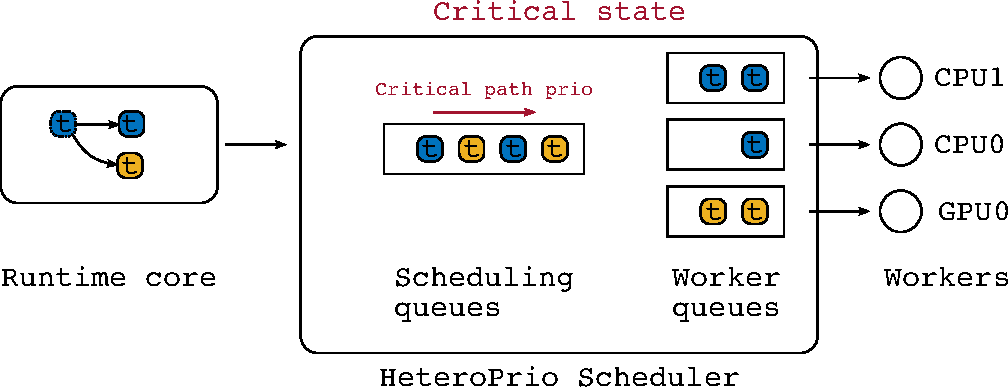
\includegraphics[width=0.8\textwidth]{figures/sched_hp_critical}}%
  \end{center}

  % \vspace{-0.5cm}

  \begin{block}{HeteroPrio: dynamic policy switching}
    \begin{itemize}
    \item<1-> \dr{Steady-state}: high concurrency $\Rightarrow$ maximize tasks acceleration
      \begin{itemize}
      \item[\dg{$\blacktriangle$}]<1-> Good matching between tasks
      and units. 
      \end{itemize}
    \item<2-> \dr{Critical-state}: low concurrency $\Rightarrow$ improve the critical path          
      \begin{itemize}
      \item[\dg{$\blacktriangle$}]<2-> Avoid stalls in the pipeline. 
      \end{itemize}
    \end{itemize}
  \end{block}
\end{frame}

\begin{frame}{Experimental results}
  \centering
  \texttt{\small
    \begin{tabular}{rlrl}
      \hline
      \# & Matrix          & Gflops & Ordering \\
      \hline
      12 & hirlam          & 1384   & SCOTCH   \\
      13 & flower\_8\_4    & 2851   & SCOTCH   \\
      14 & Rucci1          & 5671   & SCOTCH   \\
      15 & ch8-8-b3        & 10709  & SCOTCH   \\
      16 & GL7d24          & 16468  & SCOTCH   \\
      17 & neos2           & 20170  & SCOTCH   \\
      18 & spal\_004       & 30336  & SCOTCH   \\
      19 & n4c6-b6         & 62246  & SCOTCH   \\
      21 & TF18            & 194473 & SCOTCH   \\      
      \hline
      2  & karted          & 279    & COLAMD   \\
      5  & cat\_ears\_4\_4 & 786    & COLAMD   \\
      7  & e18             & 3399   & COLAMD   \\
      8  & flower\_7\_4    & 4261   & COLAMD   \\
      11 & TF17            & 38209  & COLAMD   \\
      24 & TF16            & 2884   & COLAMD   \\ 
      \hline
   \end{tabular}}
\end{frame}


\begin{frame}{Experimental results}
  {\bf System \db{Sirocco}} (Plafrim supercomputing center):

  \begin{columns}
    \begin{column}{0.5\textwidth}
      % \texttt{\tiny
      %   \begin{tabular}{rlrl}
      %     \hline
      %     \# & Matrix       & Mflops    & Ordering \\
      %     \hline
      %     12 & hirlam       & 1384160   & SCOTCH   \\
      %     13 & flower\_8\_4 & 2851508   & SCOTCH   \\
      %     14 & Rucci1       & 5671282   & SCOTCH   \\
      %     15 & ch8-8-b3     & 10709211  & SCOTCH   \\
      %     16 & GL7d24       & 16467844  & SCOTCH   \\
      %     17 & neos2        & 20170318  & SCOTCH   \\
      %     18 & spal\_004    & 30335566  & SCOTCH   \\
      %     19 & n4c6-b6      & 62245957  & SCOTCH   \\
      %     20 & sls          & 65607341  & SCOTCH   \\
      %     21 & TF18         & 194472820 & SCOTCH   \\
      %     22 & lp\_nug30    & 221644546 & SCOTCH   \\
      %     23 & mk13-b5      & 259751609 & SCOTCH   \\
      %     \hline
      %   \end{tabular}}

      
      \begin{itemize}
      \item Haswell Intel Xeon E5-2680 @ 2.5 GHz, $2\times 12$ cores
      \item 128 GB memory (NUMA)
      \item Nvidia K40 GPUs, 4 devices
      \end{itemize}

    \end{column}
    \begin{column}{0.5\textwidth}
        
        \begin{itemize}
        \item Compilers Intel ifort and icc 15.0.2
        \item BLAS and LAPACK libraries from Intel MKL 11.2.
        \end{itemize}
    \end{column}
  \end{columns}

  \begin{center}
    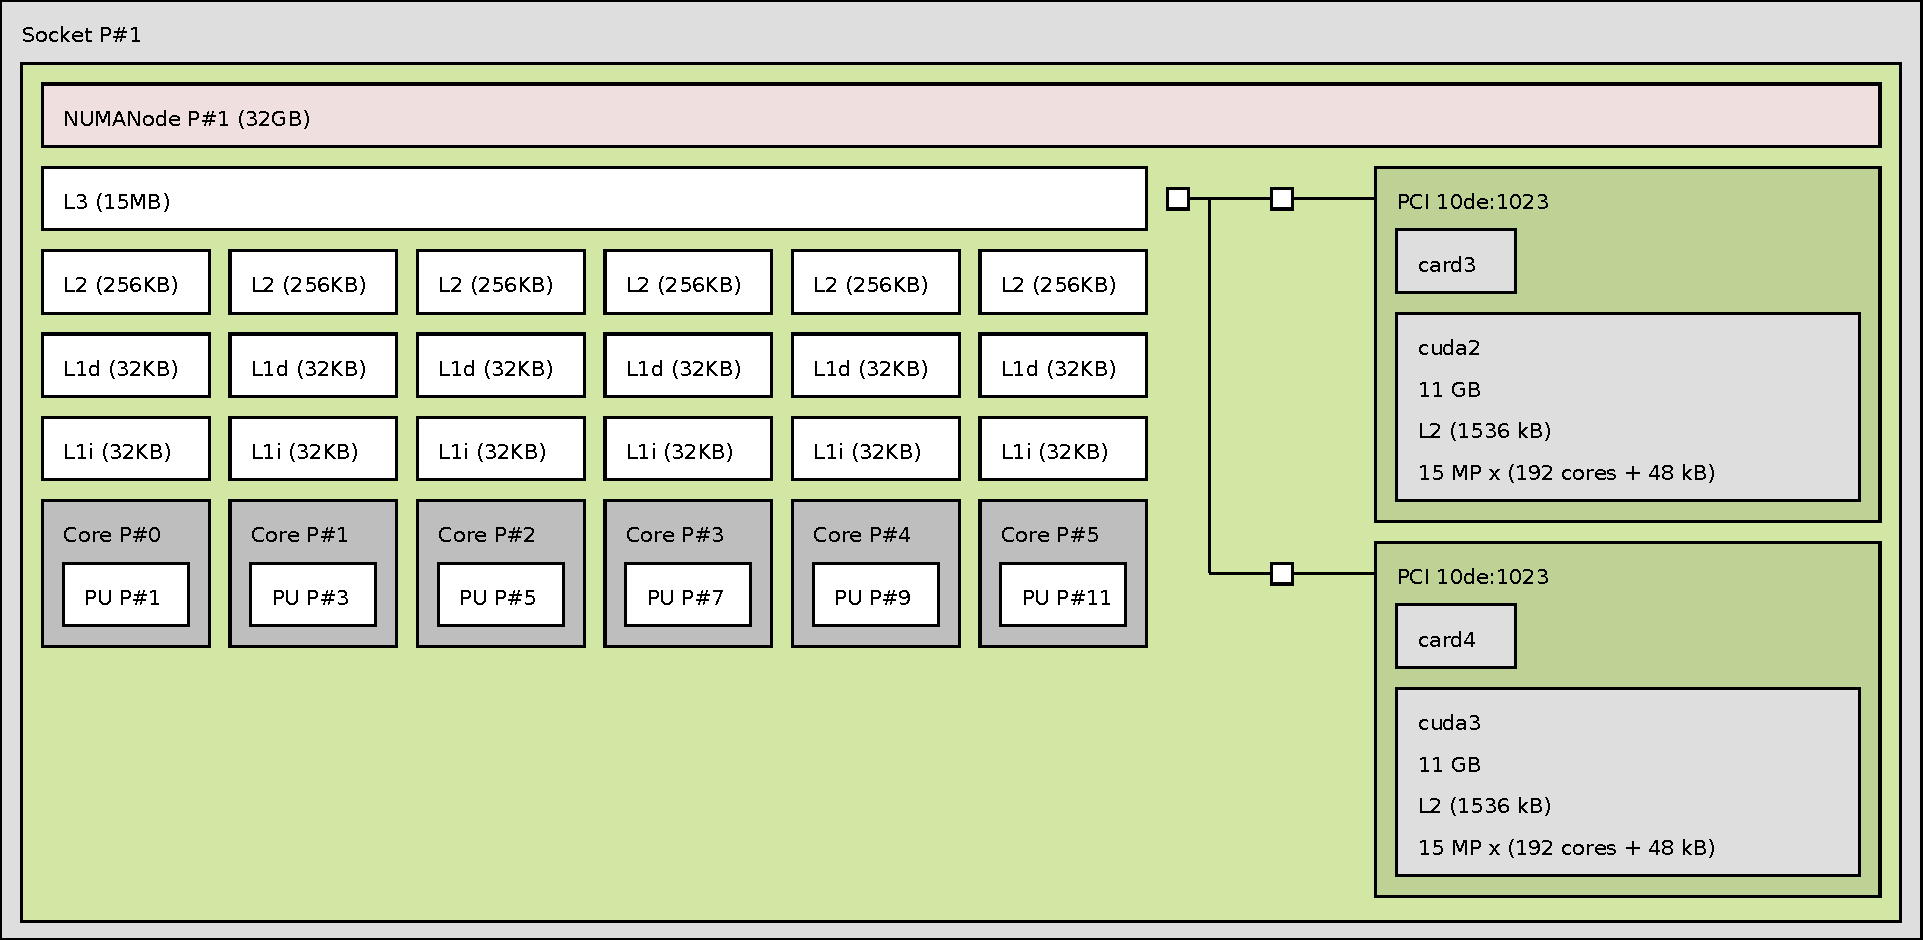
\includegraphics[width=0.8\textwidth]{figures/sirocco2}
  \end{center}

\end{frame}

\begin{frame}{Experimental results: absolute performance}
  \centering
  \only<1>{\includegraphics[width=\textwidth]{figures/perf_sirocco2_1}}%
  \only<2>{\includegraphics[width=\textwidth]{figures/perf_sirocco2_2}}%
  \only<3>{\includegraphics[width=\textwidth]{figures/perf_sirocco2_3}}%
  \only<4>{\includegraphics[width=\textwidth]{figures/perf_sirocco2_4}}%
  \only<5>{\includegraphics[width=\textwidth]{figures/perf_sirocco2}}%
\end{frame}

\begin{frame}{Area performance upper bound}

  The parallel efficiency can be defined as

  \begin{displaymath}
    e(p) = \frac{t^{min}(p)}{t(p)}
  \end{displaymath}

  where \dr{$t^{min}(p)$} is a lower bound on execution time on $p$
  resources corresponding to the \alert{best schedule} under the
  following assumptions:

  \begin{columns}
    \begin{column}{0.45\textwidth}

      \begin{enumerate}
      \item<2-> No runtime overhead and no communications.
      \item<3-> No tasks dependencies.
      \item<4-> Tasks are moldable.

        %% \item<2-> Tasks executed at asymptotic performance (\alert{maximum task granularity})
        %% \item<2-> \alert{Perfect data locality}
      \end{enumerate}

    \end{column}
    \begin{column}{0.55\textwidth}

      \begin{center}
        \only<1>{\includegraphics[width=\textwidth]{figures/lp_anim2}}%
        \only<2>{\includegraphics[width=\textwidth]{figures/lp_anim3}}%
        \only<3>{\includegraphics[width=\textwidth]{figures/lp_anim4}}%
        \only<4->{\includegraphics[width=\textwidth]{figures/lp_anim5}}%

        % \only<2>{\includegraphics[width=\textwidth]{lp_anim2}}%
      \end{center}

    \end{column}
  \end{columns}
  
  \vspace{1cm}

  \begin{overlayarea}{\textwidth}{2cm}

    \only<5>{In the heterogeneous case we have $t^{area}(p)$ is the
      solution of a \dr{linear program}.}%
    
    \only<6->{We consider \dr{$t^{area}(p)$} when there is no
      performance loss resulting from the parallelization:
      \dr{$\tilde{t}^{area}(p)$}.}%

  \end{overlayarea}

\end{frame}

\begin{frame}{A finer performance analysis}
  The execution time $t(p)$ can be decomposed in the following four
  terms:
  \begin{itemize}
  \item<1-> \db{$t_t(p)$}: the time spent executing tasks.
  \item<1-> \mye{$t_r(p)$}: the overhead of the runtime system.
  \item<1-> \dg{$t_i(p)$}: idle time.
  \item<2-> \mbp{$t_c(p)$}: the time spent performing communications.
  \end{itemize}

  The overall efficiency can thus be written as:
  
  {\tiny
\begin{align*}
  e(p) & = \frac{\tilde{t}^{area}(p)}{t(p)} =  \frac{\tilde{t}^{area}(p) \times p }{ t_t(p) + t_r(p) + t_c(p) + t_i(p) } = \frac{ \tilde{t}^{area}_t(p) }{ t_t(p) + t_r(p) + t_c(p) + t_i(p) } \\
  & =  \mre{\overbracket{\mbk{\frac{ \tilde{t}^{area}_t(p) }{ t^{area}_t(p) }}}^{e_g}}\cdot 
  \mbl{\overbracket{\mbk{\frac{ t^{area}_t(p) }{ t_t(p) }}}^{e_{t}}}\cdot  
  \mye{\overbracket{\mbk{\frac{ t_t(p) }{ t_t(p)+t_r(p) }}}^{e_r}}\cdot
  \uncover<2->{\mbp{\overbracket{\mbk{\frac{ t_t(p)+t_r(p) }{t_t(p)+t_r(p)+ t_c(p)}}}^{e_c}}\cdot}
  \mgr{\overbracket{\mbk{\frac{ t_t(p)+t_r(p)+ t_c(p) }{ t_t(p) + t_r(p) + t_c(p) + t_i(p) }}}^{e_p}}.
\end{align*}
 }
    % \begin{displaymath}
    %   \tiny
    %     e(p) = \mbk{\frac{\tilde{t}^{area}(p)}{t(p)}} 
    %     % = \frac{ \tilde{t}^{area}(p) \times p }{ t_t(p) + t_r(p) + t_c(p) + t_i(p) } = \frac{ \tilde{t}^{area}_t(p) }{ t_t(p) + t_r(p) + t_c(p) + t_i(p) }
    %     = \mre{\overbracket{\mbk{\frac{ \tilde{t}^{area}_t(p) }{ t^{area}_t(p) }}}^{e_g}}\cdot
    %     \mbl{\overbracket{\mbk{\frac{ t^{area}_t(p) }{ t_t(p) }}}^{e_{t}}}\cdot
    %     \mgr{\overbracket{\mbk{\frac{ t_t(p) }{ t_t(p)+t_r(p) }}}^{e_r}}\cdot
    %     \mbp{\overbracket{\mbk{\frac{ t_t(p)+t_r(p) }{t_t(p)+t_r(p)+ t_c(p)}}}^{e_c}}\cdot
    %     \mye{\overbracket{\mbk{\frac{ t_t(p)+t_r(p)+ t_c(p) }{ t_t(p) + t_r(p) + t_c(p) + t_i(p) }}}^{e_p}}.
    % \end{displaymath}

%   \begin{displaymath}
% e(p) = \frac{t^{area}(p)}{t(p)} =%
% \only<1,3,4,5>{\overbracket{\frac{t^{area}_t(p)}{t_t(p)}}^{e_h}}%
% \only<2>{\dr{\overbracket{\frac{t^{area}_t(p)}{t_t(p)}}^{e_h}}}%
% \cdot%
% \only<1,2,4,5>{\overbracket{\frac{t_t(p)}{t_t(p)+t_r(p)}}^{e_r}}%
% \only<3>{\dg{\overbracket{\frac{t_t(p)}{t_t(p)+t_r(p)}}^{e_r}}}%
% \cdot%
% \only<1,2,3,5>{\overbracket{\frac{t_t(p)+t_r(p)}{t_t(p)+t_r(p)+t_i(p)}}^{e_p}}%
% \only<4>{\db{\overbracket{\frac{t_t(p)+t_r(p)}{t_t(p)+t_r(p)+t_i(p)}}^{e_p}}}%
%   \end{displaymath}
  
  \vspace{0.5cm}

  with:

  \vspace{0.3cm}

  \begin{overlayarea}{\textwidth}{3cm}
    \only<2>{\mbp{$e_c$}: the \mbp{communication efficiency}. measures
      the cost of communications with respect to the actual work done
      due to data transfers between workers.}%

    \only<3>{\db{$e_t$}: the \db{task efficiency}. Measures how well
      the assignment of tasks to processing units matches the tasks
      properties to the units capabilities.}%

    % \begin{itemize}
    % \item<5> if $e_h>1$ GPUs are overloaded and CPU starve ($e_p<1$)
    % \item<5> if $e_h<1$ tasks acceleration factor not properly exploited
    % \end{itemize}%

    % \only<7>{$e_t \cdot e_p$ measures the quality of the scheduling
    % and is $\leq 1$.}
  \end{overlayarea}

\end{frame}

\begin{frame}{Experimental results: efficiency breakdown}
  \centering
  \includegraphics[width=0.9\textwidth]{data/eff_sirocco2}
\end{frame}

\begin{frame}{Experimental results: efficiency breakdown}
  \centering
  \includegraphics[width=0.9\textwidth]{data/eff_sirocco3}
\end{frame}

\begin{frame}{Experimental results: absolute performance}
  \centering
  \only<1>{\includegraphics[width=0.9\textwidth]{data/perf_multistream_sirocco2_1}}
  \only<2>{\includegraphics[width=0.9\textwidth]{data/perf_multistream_sirocco2_2}}

  \begin{itemize}
  \item A \dr{stream} is a sequence of commands that execute in order;
  \item The use of multiple stream increases the \dr{occupancy} of the
    device;
  \item Note that tasks that whose execution cannot be overlapped are
    serialized on the GPU.
  \end{itemize}
\end{frame}

\begin{frame}{Performance of multifrontal QR factorization}

  Comparison with \alert{GPU-only} SuiteSparse QR (factorization time):

  \vspace{0.3cm}

  
  \begin{center}

\begin{table}[h]
  \centering
  \begin{tabular}{llrrr}
    \toprule
    \rowcolor{bgray}
    \# & \multicolumn{2}{c}{Factorize time (s)} \\
    \rowcolor{bgray}
       & \qrm      & \spqr                      \\
    \otoprule                                                      
    2  & 1.661E+00 & 3.210E+00                  \\
    5  & 4.164E+00 & 5.469E+00                  \\
    % 6  & 9.084E+00 & $\ast$                     \\
    24 & 8.893E+00 & 1.493E+01                  \\
    7  & 8.585E+00 & 1.874E+01                  \\
    8  & 1.652E+01 & 2.254E+01                  \\
    % 9  & 2.834E+01 & $\ast$                     \\
    11 & 6.001E+01 & $\ast\ast$                 \\
    \bottomrule
  \end{tabular}
  % \caption{\label{tab:comparison-factorize-times}Factorization time
  %   for the test matrices with \qrm (24 CPU cores and 1 GPU) using
  %   multiple streams. On the last column, the factorization times for
  %   the \spqr solver. $\ast$ means that the solver returned an
  %   erroneous solution and $\ast\ast$ means that the memory
  %   requirement for these matrices  exceeded the GPU memory size.}
\end{table}

    % \begin{tabular}{l|rrrrr}
    %   \toprule
    %   & \multicolumn{5}{c}{Matrix \#}                                                                                                        \\
    %   \cmidrule(r){2-6}
    %   & 1                       & 2                       & 4                        & 5                         & 6                         \\
    %   \hline
    %   \qrm 1 stream & 2.4                     & 6.2                     & \cellcolor{gray!20}  9.4 & \cellcolor{gray!20}  14.4 & \cellcolor{gray!20}  19.8 \\
    %   \qrm 2 stream & \cellcolor{gray!20} 2.4 & 6.6                     & 10.7                     & 14.9                      & 20.6                      \\
    %   \spqr         & 2.7                     & \cellcolor{gray!20} 5.2 & 14.3                     & 18.2                      & 22.0                      \\
    %   \bottomrule
    % \end{tabular}
  \end{center}

  \begin{itemize}
  \item \qrm is competitive with a \alert{GPU-only} code despite the
    data movements.
  \item performance difference due to the use of CPUs.
  % \item on matrices 3 and 7 \spqr returned an incorrect result (likely
  %   due to a misuse of the software?).
  \item on matrices \# 11 \spqr run out of GPU memory:
    \begin{itemize}
    \item SPQR limited by maximum front (family) size.
    \item \qrm limited by maximum task size.
    % \item GPU memory is managed by the runtime system.
    \end{itemize}
  \end{itemize}

\end{frame}

%%% Local Variables:
%%% mode: latex
%%% TeX-master: "defense"
%%% TeX-engine: xetex
%%% End:

\section{Memory-aware multifrontal method}
\begin{frame}{Memory consumption}

  \begin{columns}
    \begin{column}{0.5\textwidth}

      \only<1>{\includegraphics[width=\textwidth]{figures/memmf}}%
      \only<2>{\includegraphics[width=\textwidth]{figures/memmf_factors}}%
      \only<3>{\includegraphics[width=\textwidth]{figures/memmf_cb}}%
      \only<4>{\includegraphics[width=\textwidth]{figures/memmf-opt1}}%
      \only<5>{\includegraphics[width=\textwidth]{figures/memmf-opt2}}%
      \only<6>{\includegraphics[width=\textwidth]{figures/memmf-opt3}}%
      \only<7>{\includegraphics[width=\textwidth]{figures/memmf-opt4}}%
      \only<8>{\includegraphics[width=\textwidth]{figures/memmf-opt5}}%
      \only<9>{\includegraphics[width=\textwidth]{figures/memmf-opt6}}%
      \only<10>{\includegraphics[width=\textwidth]{figures/memmf-opt7}}%
      \only<11>{\includegraphics[width=\textwidth]{figures/memmf-opt8}}%
      \only<12->{\includegraphics[width=\textwidth]{figures/memmf-opt9}}%
      
    \end{column}
    \begin{column}{0.5\textwidth}

      \begin{tabular}{r|r}
        Task & Memory \\

        \uncover<4->{\texttt{allocate(b)}}    & \uncover<4->{5}       \\
        \uncover<5->{\texttt{allocate(c)}}    & \uncover<5->{10}      \\
        \uncover<6->{\texttt{allocate(d)}}    & \uncover<6->{\dr{19}} \\
        \uncover<7->{\texttt{deallocate(b)}}  & \uncover<7->{15}      \\
        \uncover<8->{\texttt{deallocate(c)}}  & \uncover<8->{11}      \\
        \uncover<9->{\texttt{allocate(a)}}    & \uncover<9->{14}      \\
        \uncover<10->{\texttt{allocate(e)}}   & \uncover<10->{17}     \\
        \uncover<11->{\texttt{deallocate(a)}} & \uncover<11->{16}     \\
        \uncover<12->{\texttt{deallocate(d)}} & \uncover<12->{15}     \\
      \end{tabular}

    \end{column}
  \end{columns}
  
  \vspace{0.5cm}

  The memory usage varies during the factorization as the frontal
  matrices are \dr{allocated} and \dr{deallocated}. Memory usage is
  split in two:

  \begin{itemize}
    \uncover<2->{\item A \dr{persistent} memory containing the
      computed factors.}    
    \uncover<3->{\item A \dr{temporary} memory containing the
      contribution blocks, freed when a front is deallocated.}
  \end{itemize}

\end{frame}

\begin{frame}{Memory footprint in the multifrontal method}

  \begin{center}
    \only<1>{\includegraphics[width=\textwidth]{data/hirlam_ma_profile_seq}}
    \only<2->{\includegraphics[width=\textwidth]{data/hirlam_ma_profile2}}
  \end{center}

  \begin{itemize}
    \uncover<2->{\item Tree-level parallelism increases the memory
      consumption.}

    \uncover<2->{\item During a parallel execution, the memory
      consumption is generally \dr{much bigger} than the sequential
      memory consumption.}
  \end{itemize}

\end{frame}

\begin{frame}{Experimental results: memory constrained factorization}

  \begin{center}
    \includegraphics[width=\textwidth]{data/relative_mem2}
  \end{center}
  
  Two scenarios for the parallel execution:
  \begin{itemize}
  \item In-Core (IC) execution: this is the most common case where the
    computed factors are kept in memory.
  \item Out-Of-Core (OOC) execution: in this scenario the factors are
    written to disk as they are computed in order to save memory.
  \end{itemize}

\end{frame}

\begin{frame}{Task scheduling under memory constraint}

  \vspace{-1cm}

  \begin{block}{Memory-aware parallel execution}
    \alert{Objective}: achieve efficient parallel execution within a
    prescribed memory consumption
    \alert{$M_p \le \alpha M_s,~~\alpha \ge 1$}.
  \end{block}

  \uncover<2->{
    
    \vspace{0.3cm}
    
    \alert{Method}: suspend tasks submission when no more memory is
    available and resume it when enough memory has been freed by
    previously submitted tasks.}
  
    \vspace{0.3cm}
  
    \begin{columns}
      \begin{column}{0.5\textwidth}

        % \vspace{0.2cm}

        \uncover<3->{Special care must be taken to avoid \alert{memory
            deadlocks}.}

        \vspace{0.2cm}

        \uncover<4>{Example: if $M_p=1.0 M_s=19$ memory units, concurrent
        allocation of fronts \texttt{a}, \texttt{b} and \texttt{c}
        will result in a deadlock.}
      \end{column}
      \begin{column}{0.5\textwidth}
        \begin{overlayarea}{\textwidth}{2cm}
          \begin{center}
            \only<3>{\includegraphics[width=\textwidth]{figures/memmf}}%
            \only<4>{\includegraphics[width=\textwidth]{figures/memmf_par}}%
          \end{center}
        \end{overlayarea}
      \end{column}
    \end{columns}
\end{frame}

\begin{frame}{Task scheduling under memory constraint}

  \begin{block}{Deadlock prevention}
    Organize resource (memory) usage by each process to ensure that at
    least one process is always able to get all the resources it
    needs (Agullo \textit{et al.}, Marchal \textit{et al.}, Amestoy \textit{et al.}).
  \end{block}

  \uncover<2->{\alert{Approach}: the allocation of fronts is forced to
  respect the \alert{sequential order}. }
  % The tasks
  % submitted as a results of a front allocation can be executed in
  % any order.}
  
  \vspace{-0.2cm}
  
  \begin{overlayarea}{\textwidth}{4cm}
    \begin{center}
      \only<2>{\includegraphics[width=0.5\textwidth]{figures/memmf}}%
      \only<3>{\includegraphics[width=0.5\textwidth]{figures/memmf_act}}
    \end{center}
  \end{overlayarea}

  \uncover<3>{This ensures that the parallel execution can run to completion
  within the same memory envelop as the sequential one.}


\end{frame}

\begin{frame}[fragile,t,plain]{Memory aware scheduling in a STF model}

\begin{lstlisting}[basicstyle=\tt\tiny]
do f=1, nfronts ! in postorder

   call activate(f)    ! compute structure and register handles

   call submit(init, f) ! allocate and initialize front

   do c=1, f%nc ! for all the children of f
      do j=1,c%n
         ! assemble column j of c into f
         call submit(assemble, c, j, f)
      end do
      ! cleanup child
      call submit(clean, c)
   end do

   do p=1, f%n
      ! panel reduction of column p
      call submit(_geqrt, f, p)
      do u=p+1, f%n
         ! update of column u with panel p
         call submit(_gemqrt, f, u, p)
      end do
   end do
end do
! wait for the tasks to be executed
call wait_tasks_completion()
\end{lstlisting}
\end{frame}

\begin{frame}[fragile,t,plain]{Memory aware scheduling in a STF model}
\begin{lstlisting}[basicstyle=\tt\tiny]
do f=1, nfronts ! in postorder
   do while(avail_mem < size(f)) wait()
   
   call allocate(f)    ! allocate front: avail_mem -= size (f)

   call activate(f) ! compute structure and register handles
   
   call submit(init, f) ! initialize front

   do c=1, f%nc ! for all the children of f
      do j=1,c%n
         ! assemble column j of c into f
         call submit(assemble, c, j, f)
      end do
      ! cleanup child: avail_mem += size ( cb ( f ) )
      call submit(clean, c)
   end do

   do p=1, f%n
      ! panel reduction of column p
      call submit(_geqrt, f, p)
      do u=p+1, f%n
         ! update of column u with panel p
         call submit(_gemqrt, f, u, p)
      end do
   end do
end do
! wait for the tasks to be executed
call wait_tasks_completion()
\end{lstlisting}

\end{frame}

% \begin{frame}{Experimental results: memory constrained factorization}
%   \centering
%   \includegraphics[width=\textwidth]{ma_times_1d}
% \end{frame}

\begin{frame}{Experimental results: memory constrained factorization}
  \centering
  \alert{$M_p \le \alpha M_s,~~\alpha=\{1.0,1.2,1.4,1.6,1.8,2.0\}$}
  \includegraphics[width=0.95\textwidth]{data/ma_times2}
\end{frame}

% \begin{frame}{Task scheduling under memory constraint}

%   \dr{Problem}: minimize the memory footprint of the factorization.
   
%   \db{Sequential} case:
%   \begin{itemize}
%   \item Memory-minimizing postorder traversal: Liu's
%     algorithms~\cite{l:86}
%   \end{itemize}

%   \db{Parallel} case:
%   \begin{itemize}
%   \item The problem is \dr{NP-complete} and no \dr{approximation
%       algorithms} can be designed to tackle the
%     problem~\cite{e.m.s.v:15}.

%   \item \citet{e.m.s.v:15} propose several \dr{heuristics} such as
%     {\sc MemBookingInnerFirst} for the scheduling of task trees under
%     a given memory constraint.
%   \end{itemize}

% \end{frame}

% \begin{frame}{Task scheduling under memory constraint}

%   \dr{Objective}: limit the memory footprint of the parallel
%   factorization.  

%   \begin{overlayarea}{\textwidth}{1.5cm}    
%     \only<2-3>{\dr{Example}: Memory constraint: 19 memory units. }%
%     \only<3>{Let's assume that nodes \db{a}, \db{b} and \db{c} are
%       activated in parallel consuming 13 meory units and node \db{d}
%       cannot be allocated: \alert{Deadlock}.}

%     \only<4->{\dr{Approach}: the activation of fronts is forced to
%       respect the memory-minimizing sequential order. The tasks
%       submitted as a results of a front activation can be executed in
%       any order.}
%   \end{overlayarea}    

%   \begin{center}
%     \only<1-2>{\includegraphics[width=0.5\textwidth]{memmf}}%
%     \only<3>{\includegraphics[width=0.5\textwidth]{memmf3}}%
%     \only<4->{\includegraphics[width=0.5\textwidth]{memmf_act}}%
%   \end{center}  

%   \uncover<5->{This ensures that the parallel execution runs within
%     the same memory envelop as the sequential one. The memory
%     constraint can be relaxed in order to permit the activation of
%     more fronts and, potentially achieve more concurrency.}

% \end{frame}

% \begin{frame}[fragile,t,plain]{Memory aware scheduling in a STF model}

% \begin{lstlisting}[basicstyle=\tt\tiny]
% do f=1, nfronts ! in postorder

%    call activate(f)    ! compute structure and register handles

%    call submit(init, f) ! allocate and initialize front

%    do c=1, f%nc ! for all the children of f
%       do j=1,c%n
%          ! assemble column j of c into f
%          call submit(assemble, c, j, f)
%       end do
%       ! cleanup child
%       call submit(clean, c)
%    end do

%    do p=1, f%n
%       ! panel reduction of column p
%       call submit(panel, f, p)
%       do u=p+1, f%n
%          ! update of column u with panel p
%          call submit(update, f, u, p)
%       end do
%    end do
% end do
% ! wait for the tasks to be executed
% call wait_tasks_completion()
% \end{lstlisting}
% \end{frame}

% \begin{frame}[fragile,t,plain]{Memory aware scheduling in a STF model}
% \begin{lstlisting}[basicstyle=\tt\tiny]
% do f=1, nfronts ! in postorder
%    do while(avail_mem < size(f)) wait()

%    call activate(f) ! compute structure and register handles
   
%    call allocate(f)    ! allocate front: avail_mem -= size (f)

%    call submit(init, f) ! initialize front

%    do c=1, f%nc ! for all the children of f
%       do j=1,c%n
%          ! assemble column j of c into f
%          call submit(assemble, c, j, f)
%       end do
%       ! cleanup child: avail_mem += size ( cb ( f ) )
%       call submit(clean, c)
%    end do

%    do p=1, f%n
%       ! panel reduction of column p
%       call submit(panel, f, p)
%       do u=p+1, f%n
%          ! update of column u with panel p
%          call submit(update, f, u, p)
%       end do
%    end do
% end do
% ! wait for the tasks to be executed
% call wait_tasks_completion()
% \end{lstlisting}

% \end{frame}

% \begin{frame}{Experimental results: memory constrained factorization}
%   \begin{center}
%     \includegraphics[width=\textwidth]{relative_mem}
%   \end{center}
  
%   Two scenarios for the parallel execution:
%   \begin{itemize}
%   \item In-Core (IC) execution: this is the most common case where the
%     computed factors are kept in memory.
%   \item Out-Of-Core (OOC) execution: in this scenario the factors are
%     written to disk as they are computed in order to save memory.
%   \end{itemize}

% \end{frame}

% % \begin{frame}{Experimental results: memory constrained factorization}
% %   \centering
% %   \includegraphics[width=\textwidth]{ma_times_1d}
% % \end{frame}

% \begin{frame}{Experimental results: memory constrained factorization}
%   \centering
%   \includegraphics[width=\textwidth]{ma_times_2d}
% \end{frame}

%%% Local Variables:
%%% mode: latex
%%% TeX-master: "defense"
%%% TeX-engine: xetex
%%% End:

\section{Conclusion and Future Work}
\begin{frame}{Conclusions}

  \begin{block}{Conclusions}
    
    \begin{itemize}
    \item STF is suited to complex workloads and
      algorithms such as sparse matrix factorizations.

    \item The performance of the parallel execution for the STF-based
      multifrontal factorization under a memory constraint is as high as
      the unconstrained case.

      
      {\scriptsize \begin{thebibliography}{9}
        \setbeamertemplate{bibliography item}[article]
      \bibitem{a.b.g.l.:15} E. Agullo, A. Buttari, A. Guermouche, and
        F. Lopez.  \newblock Implementing multifrontal sparse solvers
        for multicore architectures with Sequential Task Flow runtime
        systems.  \newblock Submitted to ACM Transactions On
        Mathematical Software.
      \end{thebibliography}}

    \end{itemize}

  \end{block}
  
\end{frame}

\begin{frame}{Conclusions}

  \begin{block}{Conclusions}

    \begin{itemize}


    \item STF eases the implementation of GPU-based multifrontal
      method.

      {\scriptsize \begin{thebibliography}{9}
        \setbeamertemplate{bibliography item}[article]
      \bibitem{a.b.g.l.:15} E. Agullo, A. Buttari, A. Guermouche, and
        F. Lopez.  \newblock Task-based multifrontal QR solver for
        GPU-accelerated multicore architectures.  \newblock Accepted
        at the HiPC 2015 conference.
      \end{thebibliography}}

    \item Modern runtime engines are efficient and introduce a small
      (almost insignificant) overhead.

      {\scriptsize \begin{thebibliography}{9}
        \setbeamertemplate{bibliography item}[article]
      \bibitem{a.b.g.l.:13} E. Agullo, A. Buttari, A. Guermouche, and
        F. Lopez.\newblock Multifrontal {QR} Factorization for
        Multicore Architectures over Runtime Systems. \newblock In:
        Euro-Par 2013 Parallel Processing.
      \end{thebibliography}}

    \end{itemize}

  \end{block}
    
\end{frame}


\begin{frame}{Perspectives}

  \begin{block}{Associated work }
    \begin{itemize}
    \item PTG-parallel multifrontal $QR$ method implemented with the
      PaRSEC runtime system.
    \item Reproducing and simulating parallel executions of the
      multifrontal $QR$ method with StarPU SimGrid
      
      {\scriptsize \begin{thebibliography}{9}
          \setbeamertemplate{bibliography item}[article]
        \bibitem{a.b.g.l.:15} L. Stanisic, E. Agullo, A. Buttari,
          A. Guermouche, A. Legrand, F. Lopez, and B. Videau.
          \newblock Fast and Accurate Simulation of Multithreaded
          Sparse Linear Algebra Solvers. \newblock Accepted at the
          ICPADS 2015 conferece.
      \end{thebibliography}}

    \end{itemize}
  \end{block}

  \begin{exampleblock}{On-going and future work}
    
    \vspace{-0.3cm}
    
    \begin{itemize}
    \item \db{Multi-GPU} architectures.
    \item \db{Distributed} memory architectures.
    \end{itemize}
    
  \end{exampleblock}

\end{frame}

%%% Local Variables:
%%% mode: latex
%%% TeX-master: "defense"
%%% TeX-engine: xetex
%%% End:


%% Thanks

\begin{frame}[plain]{}
  \begin{center}
    \vspace{2cm}

    {\Huge Thanks!}

    \vspace{1cm}

    {\huge Questions?}

    \vspace{2cm}

  \end{center}
\end{frame}

\appendix

\AdditionalSlidesBegin

\begin{frame}[allowframebreaks]{Bibliography}
  \printbibliography[prefixnumbers=S, title={Submitted articles}, keyword=lopezsubmittedjournal]
  \printbibliography[prefixnumbers=C, title={Conference proceedings}, keyword=lopezconference]
  \printbibliography[prefixnumbers=P, title={Posters}, keyword=lopezposter]
  \printbibliography[prefixnumbers=T, title={Conference talks}, keyword=lopezpresentation]
\end{frame}

\begin{frame}[allowframebreaks]
  \printbibliography[title={References}, resetnumbers=true, notkeyword=lopez]
\end{frame}

\begin{frame}{Architectures}

  \begin{center}
    \includegraphics[width=0.9\textwidth]{data/top500}
  \end{center}

  According to the \dr{Top500 lists}, multicore
  architectures introduced in 2001 nowadays represents 100 \% of
  the performance share in the list. Accelerator, such as \db{GPU}
  and \db{Xeon Phi devices}, started gaining interests in the HPC
  community in 2005 and became very popular ever since.

\end{frame}

\begin{frame}{Tree pruning in the multifrontal method}
  The elimination tree is split in two parts using a NG\&Geist-like method:
  \begin{itemize}
  \item<2-> \dg{Top}: tree and node parallelism with hierarchical partitioning. 
  \item<4-> \db{Bottom}: sequential subtrees (only tree parallelism) with
    MAGMA-like (\alert{with staircase}), coarse-grain partitioning.
  \end{itemize}

  \vspace{0.5cm}

  \begin{center}
    \only<1>{\includegraphics[width=0.8\textwidth]{figures/lzero-0} }% 
    \only<2>{\includegraphics[width=0.8\textwidth]{figures/lzero-1} }% 
    \only<3>{\includegraphics[width=0.8\textwidth]{figures/lzero-2} }% 
    \only<4>{\includegraphics[width=0.8\textwidth]{figures/lzero-3} }% 
  \end{center}


\end{frame}

\begin{frame}{Task granularity: GPU vs CPU}
  \centering
   
  \includegraphics[width=0.9\textwidth]{figures/cholesky_GEMM_evaluation_nolog}

\end{frame}

\begin{frame}{The PTG parallel multifrontal QR factorization}
  \centering
   
  \includegraphics[width=0.4\textwidth]{figures/dag_parsec}

  Two level hierarchical DAG
  \begin{itemize}
  \item \dr{\texttt{factorization.jdf}}: the JDF representing the
    factorization DAG (Top level DAG).
  \item \dr{\texttt{qr\_1d.jdf, qr\_2d.jdf}}: the JDF files for the
    frontal matrix factorization DAGs (inner DAGs).
  \item \dr{\texttt{assembly.jdf}}: the JDF for the assembly (inner DAG)
    operations.
  \end{itemize}

\end{frame}

\begin{frame}{The PTG programming model: example}
  \begin{columns}
    \begin{column}{0.5\textwidth}    
      \lstinputlisting{listings/seq-example.c}
    \end{column}
    \begin{column}{0.5\textwidth}
      \includegraphics[width=0.7\textwidth]{figures/example_dag}
    \end{column}
  \end{columns}    
\end{frame}

\begin{frame}{The PTG programming model: example}
  \centering
  \lstinputlisting[language=C, procnamekeys={}]{listings/ptg-example.c}
\end{frame}

\begin{frame}{The PTG parallel multifrontal QR factorization}
  \centering
  \includegraphics[width=\textwidth]{data/starpu_parsec_su}
\end{frame}

\begin{frame}{Critical path analysis}
  \centering
  \includegraphics[width=0.9\textwidth]{data/cp_ada_toms_2d}

  \begin{displaymath}
    \text{max\_speedup}=\text{avg\_concurrency} = \frac{\sum_{i \in DAG}
      w_i}{\sum_{i \in CP} w_i}
  \end{displaymath}

  \begin{itemize}
  \item The \dr{DAG} used to conduct this analysis is the one related
    to the case where \dr{32 working threads} are used.
  \item The \dr{weight} of tasks is chosen to be equal to the
    \dr{execution time} measured in an execution with only one working
    thread.
  \end{itemize}

\end{frame}


\AdditionalSlidesEnd

\end{document}

%%% Local Variables:
%%% mode: latex
%%% TeX-master: t
%%% TeX-engine: xetex
%%% End:
